% Definiciones y constantes de estilo
% Clase del documento
\documentclass[a4paper,12pt,twoside,openright,titlepage]{book}

% Paquetes necesarios
\usepackage{eurosym}
\usepackage[utf8]{inputenc}
\usepackage[spanish]{babel}
\usepackage[hidelinks,colorlinks,citecolor=Fuchsia,urlcolor=blue,linkcolor=Cerulean]{hyperref}
\usepackage{listings}
\usepackage{color}
\usepackage{anysize}
\usepackage{fancyhdr}
\usepackage{cite}
\usepackage{multirow}
\usepackage{titlesec}
\usepackage[cmex10]{amsmath}
\usepackage{algorithmic}
\usepackage{textcomp}
\usepackage{enumerate}
\usepackage{fixltx2e}
\usepackage{emptypage}
\usepackage{float}
\usepackage[pdftex]{graphicx}
\usepackage{array}
\usepackage{mdwmath}
\usepackage[caption=false,font=footnotesize]{subfig}
\usepackage{fixltx2e}
\usepackage{pdfpages}
\usepackage{quotchap}
\usepackage{fancybox}
\usepackage[acronym]{glossaries}
\usepackage{appendix}
\usepackage{bookmark}

% Euro (€)
\DeclareUnicodeCharacter{20AC}{\euro}

% Estilo de la bibliografía
\bibliographystyle{IEEEtran}

% Inclusión de gráficos
\graphicspath{{./graphics/}}

% Extensiones de gráficos
\DeclareGraphicsExtensions{.pdf,.jpeg,.jpg,.png}

% Definiciones de colores (para hidelinks)
\definecolor{LightCyan}{rgb}{0,0,0}
\definecolor{Cerulean}{rgb}{0,0,0}
\definecolor{Fuchsia}{rgb}{0,0,0}

% Keywords (español e inglés)
\def\keywordsEn{\vspace{.5em}
{\textbf{\textit{Key words ---}}\,\relax%
}}
\def\endkeywordsEn{\par}

\def\keywordsEs{\vspace{.5em}
{\textbf{\textit{Palabras clave ---}}\,\relax%
}}
\def\endkeywordsEs{\par}


% Abstract (español e inglés)
\def\abstractEs{\vspace{.5em}
{\textbf{\textit{Resumen ---}}\,\relax%
}}
\def\endabstractEs{\par}

\def\abstractEn{\vspace{.5em}
{\textbf{\textit{Abstract ---}}\,\relax%
}}
\def\endabstractEn{\par}

% Estilo páginas de capítulos
\fancypagestyle{plain}{
\fancyhf{}
\fancyfoot[CO]{\footnotesize\emph{\nombretrabajo}}
\fancyfoot[RO]{\thepage}
\renewcommand{\footrulewidth}{.6pt}
\renewcommand{\headrulewidth}{0.0pt}
}

% Estilo resto de páginas
\pagestyle{fancy}

% Estilo páginas impares
\fancyfoot[CO]{\footnotesize\emph{\nombretrabajo}}
\fancyfoot[RO]{\thepage}
\rhead[]{\leftmark}

% Estilo páginas pares
\fancyfoot[CE]{\emph{\pieparcen}}
\fancyfoot[LE]{\thepage}
\fancyfoot[RE]{\pieparizq}
\lhead[\leftmark]{}

% Guía del pie de página
\renewcommand{\footrulewidth}{.6pt}

% Nombre de los bloques de código
\renewcommand{\lstlistingname}{Código}

% Definiciones de funciones para los títulos
\newlength\salto
\setlength{\salto}{3.5ex plus 1ex minus .2ex}

\newlength\resalto
\setlength{\resalto}{2.3ex plus.2ex}

% Corrección warning
\setlength{\headheight}{15pt} 

% Estilo de sección
\newcommand{\lsection}[1]
                {\section{#1}
                \vskip-.9\resalto % Corrección del posible salto por defecto de \section
                \hrule
                \vskip+.9\salto} % Vuelvo ha realizar el salto

% Estilo de los acrónimos
\renewcommand{\acronymname}{Glosario}
\renewcommand{\glossaryname}{Glosario}
\pretolerance=2000
\tolerance=3000

% Pie de tabla
\addto\captionsspanish{
\def\tablename{Tabla}
\def\listtablename{\'Indice de tablas}
}

% Traducir appendix/appendices
\renewcommand\appendixtocname{Apéndices}
\renewcommand\appendixpagename{Apéndices}

% Definiciones de comandos
\newcommand{\nombreautor}{Juan Sidrach de Cardona Mora}
\newcommand{\nombretutor}{Dr. Sergio López-Buedo}
\newcommand{\nombretrabajo}{Interfaz web para la gestión de sondas de red de altas prestaciones}
\newcommand{\fecha}{Junio 2015}
\newcommand{\grado}{Doble Grado en Ingeniería Informática y Matemáticas}
% Descomentar si tu trabajo tiene un ponente
%\newcommand{\nombreponente}{Nombre del ponente}
\newcommand{\grupoInvestigacion}{High-Performance Computing and Networking Research Group}
\newcommand{\departamento}{Dpto. de Tecnología Electrónica y de las Comunicaciones}
\newcommand{\facultad}{Escuela Politécnica Superior}
\newcommand{\universidad}{Universidad Autónoma de Madrid}
\newcommand{\pieparizq}{\href{https://github.com/JSidrach/NetWatcher}{\scriptsize{github.com/JSidrach/NetWatcher}}}
\newcommand{\pieparcen}{Trabajo de Fin de Grado}
\newcommand{\logoizq}{Logo_EPS}
\newcommand{\logoder}{Logo_UAM}
\newcommand{\correo}{***REMOVED***}

% Glosario y acrónimos
\makeglossaries
% Acrónimos

\newacronym{HTTP}{HTTP}{Hypertext Transfer Protocol}
\newacronym{URL}{URL}{Uniform Resource Locator}
\newacronym{FPGA}{FPGA}{Field-Programmable Gate Array}
\newacronym{IFG}{IFG}{InterFrame Gap (pausa temporal entre paquetes)}
\newacronym{RAID}{RAID}{Redundant Array of Independent Disks}
\newacronym{pcap}{pcap}{Packet capture (formato de traza, utilizado por programas como \textit{Wireshark} y \textit{tcpdump})}
\newacronym{API}{API}{Application Programming Interface (métodos públicos de una aplicación)}
\newacronym{JSON}{JSON}{JavaScript Object Notation}
\newacronym{PHP}{PHP}{PHP Hypertext Pre-processor}
\newacronym{AJAX}{AJAX}{Asynchronous JavaScript and XML}

% Glosario

\newglossaryentry{bitstream}{name={bitstream},description={En este contexto se refiere al binario que configura el Hardware de la FPGA}}
\newglossaryentry{traza}{name={traza},plural={trazas},description={Archivo que contiene paquetes de red capturados}}
\newglossaryentry{simple}{name={simple},description={Formato de traza que acepta la FPGA utilizada}}
\newglossaryentry{servicioweb}{name={Servicio Web},description={Conjunto de métodos remotos accesibles a través de la red}}
\newglossaryentry{proxy}{name={proxy},description={Servidor que sirve de intermediario entre las peticiones de recursos que realiza un cliente a otro servidor}}
\newglossaryentry{framework}{name={framework},description={Entorno software que proporciona una funcionalidad base para facilitar la organización y desarrollo de aplicaciones}}
\newglossaryentry{back-end}{name={back-end},description={Componentes internos de la aplicación que procesan los datos provenientes del front-end}}
\newglossaryentry{front-end}{name={front-end},description={Interfaz, parte de la aplicación que interacciona directamente con el usuario}}
\newglossaryentry{script}{name={script},plural={scripts},description={Programa interpretado que se almacena en un archivo de texto plano}}

% Rerefencias
\bibliography{src/referencias}

% Inicio del documento
\begin{document}

% Elección del idioma (español)
\selectlanguage{spanish}

%
% Portada
%
\pagenumbering{gobble}
%
% Portada
%

% Universidad, Facultad
\begin{titlepage}
\selectlanguage{spanish}
\begin{center}
\textbf{\begin{huge}
\universidad \\
\end{huge}}
\bigskip
\begin{LARGE}
\facultad \\
\end{LARGE}
\end{center}

\bigskip
\bigskip

%
% Imágenes (logos) izquierdo y derecho
%
\begin{figure}[h]
  \begin{center}
    \includegraphics[scale=0.35]{\logoizq}
    \hspace{1cm}
    \includegraphics[scale=0.4]{\logoder}
  \end{center}
\end{figure}

\bigskip
\bigskip
\bigskip

% Grado
\begin{center}
\begin{large}
\textbf{\grado}\\
\end{large}
\end{center}

\bigskip

\textbf{\begin{center}
\begin{huge}
\MakeUppercase{Trabajo de Fin de Grado}
\end{huge}
\end{center}}

\bigskip
\bigskip

% Nombre del TFG
\begin{center}
\textbf{\begin{large}
\MakeUppercase{\nombretrabajo}\\
\end{large}}
\end{center}

% Nombre del autor
\vspace{\fill}
\begin{center}
\textbf{\nombreautor}\\
% Tutor
\textbf{Tutor: \nombretutor}\\
% Ponente, si está definido en main.tex
\ifcsname nombreponente\endcsname
\textbf{Ponente: \nombreponente}\\
\fi

\bigskip

% Fecha
\textbf{\fecha}\\
\end{center}
\end{titlepage}

% Primera página
\pagenumbering{Alph}
\thispagestyle{empty}
\par\vspace*{\fill}
\begin{flushleft}
\begin{scriptsize}
\end{scriptsize}\end{flushleft}
\newpage
\thispagestyle{empty}
\begin{center}

% Nombre del trabajo
\textbf{\begin{large}
\MakeUppercase{\nombretrabajo}\\*
\end{large}}
\vspace*{0.2cm}
\vspace{5cm}

% Nombre del autor y del tutor
\large Autor: \nombreautor \\*
\large Tutor: \nombretutor \\*
\ifcsname nombreponente\endcsname
\large Ponente: \nombreponente\\
\fi

\vfill

% Grupo de investigación, departamento, facultad, universidad y fecha
\ifcsname grupoInvestigacion\endcsname
\grupoInvestigacion \\
\fi
\departamento \\
\facultad \\
\universidad \\
\vspace{1cm}
\fecha \\

\clearpage

\end{center}
\normalsize

\hypersetup{pageanchor=true}

% Estilo de párrafo de los capítulos
\setlength{\parskip}{0.75em}
\renewcommand{\baselinestretch}{1.25}
%
% Agradecimientos
%
\pagenumbering{Roman}
\setcounter{page}{0}
\chapter*{Agradecimientos}

TODO: Agradecimientos.

Lorem ipsum dolor sit amet, consectetur adipiscing elit. Phasellus laoreet dolor at sodales porta. Morbi facilisis hendrerit lacus vel sollicitudin. Aenean eleifend urna metus, eget vestibulum libero dictum tincidunt. Curabitur quis ultrices lorem. Duis ultricies, eros eget condimentum pharetra, tellus eros lobortis nulla, vel mattis nibh dui et felis. Interdum et malesuada fames ac ante ipsum primis in faucibus. Nam non lorem et ligula condimentum molestie. Fusce quis dolor non metus suscipit commodo. Praesent vel pulvinar lectus. Nullam ac dui eget magna accumsan volutpat. Aliquam sed purus quis lorem dictum rutrum auctor eu enim. Pellentesque a urna ac ligula cursus lacinia. Aenean sodales justo massa, vel imperdiet justo imperdiet ut. Nulla euismod pulvinar arcu eu convallis. Vivamus a tempus nunc, et vulputate nulla.

Sed dapibus aliquam imperdiet. Vivamus est quam, fermentum vitae augue id, ultricies tincidunt massa. Praesent tincidunt ex sem, ut aliquet nulla imperdiet eu. Duis ac ultricies lorem. Aenean consequat ipsum nec arcu aliquam, sit amet interdum quam tempus. In justo odio, bibendum vel nulla nec, aliquet tristique justo. In vel metus ut libero suscipit ultricies.

Class aptent taciti sociosqu ad litora torquent per conubia nostra, per inceptos himenaeos. Proin urna elit, iaculis id quam at, pretium laoreet ipsum. Phasellus ultricies faucibus ex et eleifend. Quisque facilisis erat dolor, ac rhoncus erat convallis et. Aliquam semper eleifend imperdiet. Sed eros ipsum, sagittis in pellentesque vel, vestibulum a augue. Duis sapien mauris, fringilla a tortor ut, sollicitudin volutpat nunc. Pellentesque vestibulum vel arcu in molestie. Nullam fermentum dolor luctus metus efficitur pulvinar. Pellentesque risus enim, tempus id ullamcorper in, maximus id nisl. Cras rhoncus consequat augue eu gravida. Ut efficitur mauris vitae orci dignissim sagittis. Suspendisse vitae massa eget nunc bibendum interdum.

% Cita
\begin{flushright}
\textit{``In the beginning the Universe was created.
This has made a lot of people very angry and been widely regarded as a bad move.''}
-- Douglas Adams
\end{flushright}


%
% Resumen
%
% Resumen en inglés
\chapter*{Abstract}

\begin{abstractEn}

A network probe is a device capable of capturing or injecting network traffic.
This work is founded on a custom-made FPGA based probe.
So far, the only possibility to interact with this probe was through the command line, difficulting the management of the probe for people without any previous knowledge of it.
Another issue present in the probe's control was the existence of many aspects related to its operation that were being handled externally, such as storage, sorting and managing the traces or monitoring the system performance.

The proposed application facilitates the use of the network probe through a web-based graphical interface.
This interface allows the user to manage the probe without any specific knowledge of its inner workings.
In addition, it brings together other relevant aspects of the capture and injection of web traffic, such as trace storage, write speed of the disks or trace format conversion.
The interface implementation follows a responsive design and can be used on mobile devices with a similar user experience.
The final product provides an elegant interface to manage all the relevant aspects of the probe, which displays the state and additional information of the system visually, using graphs and statistics.

This project, however, has not exclusively consisted in the development of a graphical interface.
A base architecture, which formalizes the management of network probes from a web interface, has also been designed.
This proposal contemplates how to structure the components so that it is extensible to other network probes, not just the one selected.
With this goal in mind, the system has been divided into two components, back-end and front-end, which communicate with each other and that can be hosted on different servers.
Thereby, a REST Web Service has been designed and implemented for the back-end, which formalizes the status and functionality of the FPGA, adding also control over other important aspects mentioned above.
For the front-end, an ad hoc framework has been created, which has served as a starting point for the web interface.
It is intended that most of the proposed solution could be reused in similar projects, in which the management of the probes is done through command line.

\end{abstractEn}

% Palabras clave en inglés
\begin{keywordsEn}
web interface, responsive design, web service, API REST, capture and reproduction of network traffic, FPGA.
\end{keywordsEn}

% Resumen en español
\chapter*{Resumen}

\begin{abstractEs}

Una sonda de red es un dispositivo capaz de capturar tráfico de red o de inyectarlo.
Este trabajo está basado en una sonda a medida sobre una FPGA.
Hasta ahora, la única posibilidad era interaccionar con esta sonda desde la línea de comandos, lo que dificultaba su gestión para personas sin conocimientos previos de la misma.
Otro problema presente en el control de la sonda era la existencia de numerosos aspectos relacionados con su funcionamiento que se manejaban de forma externa, tales como el almacenamiento, clasificación y gestión de las trazas, o la monitorización del rendimiento del sistema.

La aplicación propuesta facilita la utilización de la sonda de red mediante una interfaz gráfica basada en tecnologías web.
Esta interfaz permite gestionar la sonda sin tener un conocimiento específico de su funcionamiento interno.
También agrupa otros aspectos relevantes de la captura y reproducción de tráfico web, como el almacenamiento de las trazas, la velocidad de escritura en disco o la conversión entre formatos de traza.
La implementación de la interfaz sigue un diseño responsive, pudiendo utilizarse desde dispositivos móviles con una experiencia de usuario similar.
Se ha conseguido, como producto final, una interfaz elegante que permite gestionar todos los aspectos de la sonda considerados relevantes, presentando el estado e información adicional del sistema de forma visual, mediante gráficos y estadísticas.

Este proyecto, sin embargo, no ha consistido únicamente en el desarrollo de una interfaz gráfica.
Se ha diseñado también una arquitectura base que formaliza la gestión de sondas de red desde una interfaz web.
Esta propuesta contempla cómo estructurar los componentes de forma que sea extensible a otras sondas de red, no solo la seleccionada.
Con este objetivo, se ha dividido el sistema en dos componentes, back-end y front-end, que se comunican entre sí y que pueden estar alojados en un servidor distinto cada uno.
Así, se ha diseñado e implementado un Servicio Web REST en el back-end, que formaliza el estado y funcionalidad de la FPGA, añadiendo también control sobre otros aspectos relevantes mencionados anteriormente.
Para el front-end se ha creado un framework propio, que ha servido de punto de partida para la interfaz web.
Se pretende que gran parte de la solución propuesta sea reutilizable en proyectos similares, en los que el manejo de las sondas se realiza por línea de comandos.

\end{abstractEs}

% Palabras clave en español
\begin{keywordsEs}
interfaz web, diseño responsive, servicio web, API REST, captura y reproducción de tráfico de red, FPGA.
\end{keywordsEs}


%
% Glosario
%
\printglossary[title=Glosario,toctitle=Glosario]
\printglossary[title=Acrónimos,toctitle=Acrónimos,type=\acronymtype]

% Estilo de párrafo de los índices
\setlength{\parskip}{1pt}
\renewcommand{\baselinestretch}{1}
%
% Tabla de contenidos
%
\tableofcontents
\listoftables
\listoffigures
\cleardoublepage

% Estilo de párrafo de los capítulos
\setlength{\parskip}{0.75em}
\renewcommand{\baselinestretch}{1.25}
% Interlineado simple
\spacing{1}
% Numeración contenido
\pagenumbering{arabic}
\setcounter{page}{1}

%
% Capítulos
%
\section{Introducción}

% Sondas de red
\begin{frame}{Sondas de red}
  \begin{itemize}
    \item\alert<+>{Dispositivos capaces de capturar y/o inyectar tráfico de red}
    \item\alert<+>{Principales usos}
    \begin{itemize}
      \item Análisis de las trazas capturadas por la sonda
      \item Realización de pruebas sobre redes, plataformas y aplicaciones
    \end{itemize}
    \item\alert<+>{Diferentes tipos sobre ordenadores convencionales}
    \begin{itemize}
      \item Tarjetas Ethernet estándar
      \item Tarjetas a medida basadas en FPGAs
    \end{itemize}
  \end{itemize}
\end{frame}

% Sonda utilizada
\begin{frame}{Sonda utilizada}
  \begin{itemize}
    \item\alert<+>{Sonda a medida basada en FPGA}
    \item\alert<+>{Permite capturar y reproducir tráfico de red}
    \item\alert<+>{Rendimiento máximo de 10 Gbps}
    \begin{itemize}
      \item Puede verse limitado por la velocidad del disco
    \end{itemize}
    \item\alert<+>{Gestionada por línea de comandos}
  \end{itemize}
\end{frame}

\section{Estado del arte}

% OSNT
\begin{frame}{The Open Source Network Tester}
  \begin{itemize}
    \item\alert<+>{Sistema de captura y reproducción de código abierto}
    \item\alert<+>{Utiliza cuatro FPGAs}
    \begin{itemize}
      \item Mismo modelo que la empleada en este TFG
    \end{itemize}
    \item\alert<+>{Gestionadas desde una interfaz sobre el propio servidor}
    \item\alert<+>{Se han identificado algunos aspectos mejorables}
    \begin{itemize}
      \item Provee información exclusivamente de la FPGA
      \item Interfaz poco intuitiva
      \item Se maneja desde el propio servidor
    \end{itemize}
    \item\alert<+>{Otras aplicaciones consideradas}
    \begin{itemize}
      \item tcpdump/libpcap
      \item Wireshark
      \item Detect-Pro
    \end{itemize}
  \end{itemize}
\end{frame}

% OSNT - Interfaz
\begin{frame}{The Open Source Network Tester - Interfaz}
  \begin{figure}
    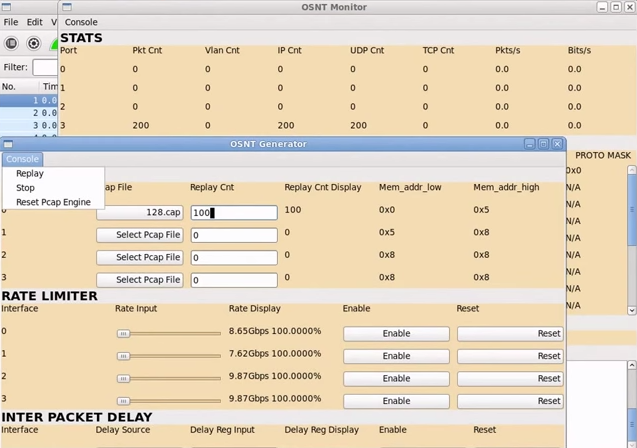
\includegraphics[width=0.9\linewidth]{osnt}
  \end{figure}
\end{frame}

\chapter{Definición del proyecto\label{cap:defProyecto}}

En este capítulo se definirán y explicarán el alcance del proyecto, la metodología de desarrollo escogida y las herramientas utilizadas.

\section{Alcance\label{sec:dp:alcance}}

Esta aplicación tiene como objetivo permitir, mediante una interfaz web, gestionar una sonda de red y conocer su estado actual.
Asimismo, posibilitará manejar otros aspectos relacionados con la sonda, como el almacenamiento y gestión de las \glspl{traza} capturadas.
Estos aspectos son comunes a cualquier sistema de captura y reproducción de tráfico de red, por lo que se estructurará la aplicación de forma que generalice el problema dado, sirviendo como trabajo base para la creación de interfaces gráficas sobre sondas similares.

No se pretende sin embargo, dentro del contexto de este proyecto, que la interfaz web sea capaz de interactuar con cualquier tipo de sonda de captura y reproducción de tráfico de red, sino solo con la sonda seleccionada.
Tampoco entra dentro del alcance de este proyecto modificar el funcionamiento interno de la sonda, ni siquiera para mejorar su rendimiento, ya que el objetivo principal es facilitar la gestión de una sonda de red de altas prestaciones y de otros componentes que intervienen en el sistema.

\section{Metodología\label{sec:dp:metodologia}}

Para el desarrollo de la aplicación se ha optado por seguir un ciclo de vida en cascada con retroalimentación.
Este modelo ordena las etapas del proceso de desarrollo software, de forma que solo se pueda iniciar una fase cuando se ha finalizado la anterior.
Dada la naturaleza de este proyecto, era necesario un periodo amplio de estudio del problema a resolver antes de poder codificar nada, siendo por ello este modelo más recomendable que adoptar alguna metodología ágil.
Por otra parte, se ha descartado utilizar un modelo iterativo o en espiral dado que conllevaría un mayor tiempo de desarrollo al tener que realizarse por módulos y de forma separada cada una de las fases definidas, en vez de simultáneamente y de forma global.
Además, el hecho de tener retroalimentación permite volver a etapas anteriores en caso de que sea necesario corregir algún aspecto del sistema.

La distribución temporal de las tareas y sus dependencias se resumen en el diagrama de Gantt de la Figura~\ref{fig:gantt}.
A continuación se detallan la entradas, tareas y salidas de cada una de las fases del desarrollo del proyecto.

\begin{figure}[!htp]
  \centering
  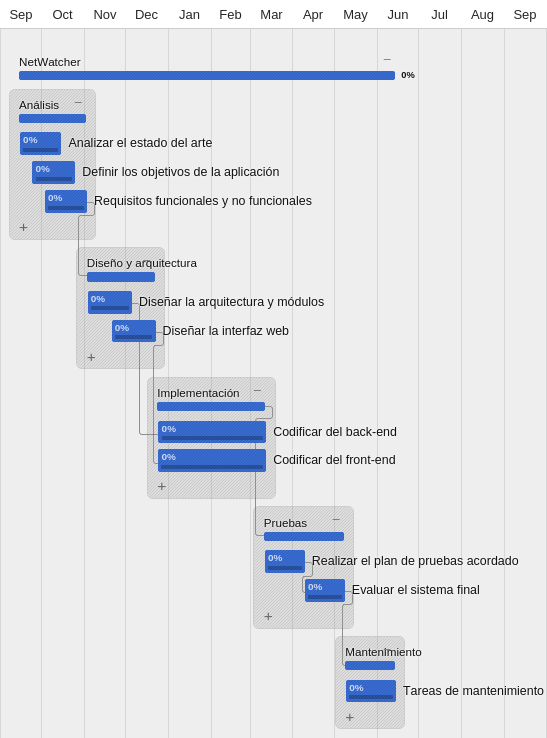
\includegraphics[width=0.7\textwidth,clip=true]{graphics/gantt_white}
  \caption{Diagrama de Gantt de la planificación temporal del proyecto}
  \label{fig:gantt}
\end{figure}

\subsection*{Análisis\label{ssec:dp:analisis}}

Tareas
\begin{itemize}[leftmargin=3.5em]
  \item Analizar el estado del arte.
  \item Definir los objetivos de la aplicación.
  \item Especificar los requisitos funcionales y no funcionales.
\end{itemize}

Salida
\begin{itemize}[leftmargin=3.5em]
  \item Definición, objetivos y alcance del proyecto.
  \item Relación de requisitos.
\end{itemize}

\subsection*{Diseño y arquitectura\label{ssec:dp:disenho}}

Entrada
\begin{itemize}[leftmargin=3.5em]
  \item Relación de requisitos.
\end{itemize}

Tareas
\begin{itemize}[leftmargin=3.5em]
  \item Diseñar la arquitectura y módulos a implementar.
  \item Diseñar la interfaz web.
\end{itemize}

Salida
\begin{itemize}[leftmargin=3.5em]
  \item Arquitectura de la aplicación.
  \item Diagramas de diseño.
  \item Maquetas de la interfaz web.
\end{itemize}

\subsection*{Implementación\label{ssec:dp:implementacion}}

Entrada
\begin{itemize}[leftmargin=3.5em]
  \item Información sobre la arquitectura y el diseño de la aplicación.
  \item Maquetas de la interfaz web.
\end{itemize}

Tareas
\begin{itemize}[leftmargin=3.5em]
  \item Codificar del \gls{back-end}.
  \item Codificar del \gls{front-end}.
\end{itemize}

Salida
\begin{itemize}[leftmargin=3.5em]
  \item Código de la aplicación.
  \item Documentación del código de la aplicación.
\end{itemize}

\subsection*{Pruebas\label{ssec:dp:pruebas}}

Entrada
\begin{itemize}[leftmargin=3.5em]
  \item Código de la aplicación.
\end{itemize}

Tareas
\begin{itemize}[leftmargin=3.5em]
  \item Realizar el plan de pruebas acordado.
  \item Evaluar el sistema final.
\end{itemize}

Salida
\begin{itemize}[leftmargin=3.5em]
  \item Código de la aplicación validado y verificado.
\end{itemize}

\subsection*{Mantenimiento\label{ssec:dp:mantenimiento}}

Entrada
\begin{itemize}[leftmargin=3.5em]
  \item Código de la aplicación validado y verificado.
\end{itemize}

Tareas
\begin{itemize}[leftmargin=3.5em]
  \item Analizar, implementar y probar las solicitudes de mejoras propuestas por usuarios.
\end{itemize}

Salida
\begin{itemize}[leftmargin=3.5em]
  \item Código de la aplicación validado y verificado, con cambios menores propuestos por usuarios.
\end{itemize}


\section{Herramientas\label{sec:dp:herramientas}}

Para el desarrollo de este proyecto han sido necesarias herramientas que cubran las siguientes necesidades:

\begin{itemize}
  \item Control de versiones.
  \item Creación de diagramas y maquetas.
  \item Documentación de la aplicación.
  \item Plataforma base para el \gls{back-end}.
  \item Plataforma base para el \gls{front-end}.
\end{itemize}

A continuación se especifican las herramientas elegidas, exponiendo su utilidad.
Se detallan también otras librerías externas de las que hace uso la aplicación.

\subsection*{Control de versiones: GitHub\label{ssec:dp:github}}

En todo proyecto software es fundamental, especialmente si se alarga en el tiempo, hacer uso de una herramienta de control de versiones para el código y la documentación.
Se ha elegido con este propósito utilizar la plataforma \textit{GitHub}~\cite{github}, basada en \textit{git}~\cite{git}, un sistema distribuido de control de versiones.
Esta plataforma es la más popular dentro de las herramientas de control de versiones, y tiene algunas ventajas importantes respecto a otros sistemas similares.

En primer lugar, ofrece alojamiento gratuito para proyectos de \gls{codigoabierto}, y también para proyectos privados si se es estudiante.
Gracias a esto se ha podido desarrollar todo el código de la aplicación en un proyecto privado, liberándolo al público al finalizar el desarrollo principal, de forma que cualquiera pueda utilizar y mejorar el código existente.
Por otra parte, \textit{GitHub} añade a la funcionalidad de \textit{git} la posibilidad de crear una \textit{wiki} del proyecto de forma sencilla, característica que ha sido utilizada en el proyecto.
Finalmente, facilita la colaboración entre desarrolladores con una interfaz intuitiva y cuya curva de aprendizaje no tiene una una pendiente demasiado elevada.

\subsection*{Creación de diagramas y maquetas: Cacoo\label{ssec:dp:cacoo}}

Para el diseño de la aplicación se han realizado diagramas de flujo y de arquitectura del proyecto, así como maquetas de las diferentes pantallas de la interfaz web.
Para ello, se ha utilizado la herramienta \textit{Cacoo}~\cite{cacoo}, ya que ofrece una licencia gratuita para estudiantes que permite exportar estos gráficos en formato vectorial \textit{svg}, que se pueden redimensionar sin pérdida de resolución.
Otra característica interesante es que está basada en tecnologías web, con lo que es accesible desde cualquier navegador, sin ser necesario instalar ningún programa adicional.

\subsection*{Documentación: phpDocumentor y apiDoc\label{ssec:dp:docs}}

Con el objetivo de documentar la aplicación, se buscó una librería que contase con características particulares.
Por un lado, que permitiese crear la documentación mediante anotaciones en el propio código, sin ralentizar demasiado la implementación del proyecto.
Por otro, que generase la documentación en formato \gls{HTML}, para que se pudiese acceder a ella del mismo modo que a la aplicación, desde un navegador.
Debido a diferencias significativas (en arquitectura y lenguaje) entre el \gls{back-end} y el \gls{front-end}, se ha decidido finalmente utilizar una herramienta de documentación distinta para cada parte.

Para el \gls{back-end} se ha elegido \textit{apiDoc}~\cite{apidoc}, ya que es multilenguaje y encaja perfectamente dentro de la arquitectura interna (ver sección~\ref{sec:dis:servicio_web_fpga}).
Respecto al \gls{front-end}, se ha seleccionado \textit{phpDocumentor}~\cite{phpdocumentor}, al tener una sintaxis similar a \textit{javadoc}, herramienta utilizada en asignaturas del grado.

\subsection*{Plataforma base para el back-end: node.js\label{ssec:dp:back-end}}

Se ha seleccionado \textit{node.js}~\cite{nodejs} como \gls{framework} \gls{back-end}.
Esta plataforma de \gls{codigoabierto} se ha considerado idónea para el proyecto por diversos motivos.
Para empezar, utiliza \textit{JavaScript}~\cite{javascript}, lenguaje conocido por el estudiante.
El hecho de que esté en este lenguaje permite además que se reutilice código entre el \gls{back-end} y el \gls{front-end}, ya que es el empleado por los navegadores web.
Otra ventaja es que detrás de \textit{node.js} existe una comunidad enorme, por lo que existen multitud de librerías también de \gls{codigoabierto} disponibles y bien documentadas.
Por último, es un \gls{framework} de programación asíncrona (en la que no se tenía experiencia), por lo que su aprendizaje ha sido muy enriquecedor.

\subsection*{Librerías utilizadas para el back-end\label{ssec:dp:back-end-libs}}

Se han utilizado las siguientes librerías \gls{back-end} de \gls{codigoabierto} para \textit{node.js}:

\begin{itemize}
  \item \textbf{Express}~\cite{express}: \gls{framework} minimalista para aplicaciones web con arquitectura \gls{REST}.

  \item \textbf{Async}~\cite{async}: módulo que proporciona funciones para trabajar asíncronamente en \textit{JavaScript}.

  \item \textbf{nodemon}~\cite{nodemon}: supervisor que monitoriza cambios en el código de la aplicación y reinicia el servidor automáticamente.

\end{itemize}

\subsection*{Plataforma base para el front-end: framework propio\label{ssec:dp:front-end}}

Se ha optado por desarrollar un \gls{framework} propio en \gls{PHP} como plataforma base para el \gls{front-end} (ver apéndice~\ref{extra:frameworkDesarrollado}).
Esta decisión está fundamentada en varios motivos.
Por un lado, no se quería utilizar un \gls{framework} que tuviese funcionalidades no necesarias para esta aplicación concreta, y cuya curva de aprendizaje ralentizase el proyecto.
Otra razón es que conocer al detalle el \gls{framework} utilizado ha proporcionado una mayor flexibilidad en el proceso de desarrollo, pudiendo además modificar la estructura y arquitectura del mismo para que se adecuase perfectamente a las necesidades propias.
Finalmente, se contaba ya con cierta experiencia programando en \gls{PHP}, por lo que ha sido el lenguaje elegido.

\subsection*{Librerías utilizadas para el front-end\label{ssec:dp:front-end-libs}}

Además del \gls{framework} desarrollado, se han utilizado diversas librerías \gls{front-end}, todas ellas de \gls{codigoabierto}.
A continuación se enumeran, describiendo brevemente su propósito:

\begin{itemize}
  \item \textbf{Bootstrap}~\cite{bootstrap}: facilita el desarrollo de aplicaciones web \textit{responsive}~\cite{responsive} mediante plantillas de diseño con tipografía, formularios, botones, cuadros y menús.

  \item \textbf{Bootstrap table}~\cite{bootstraptable}: mejora las tablas de \textit{Bootstrap} permitiendo de manera sencilla insertar un campo de búsqueda, filtrar filas por \textit{checkbox} o \textit{radio button}, ordenar por columnas, paginar automáticamente los resultados, etc.

  \item \textbf{Bootswatch}~\cite{bootswatch}: colección de temas visuales para \textit{Bootstrap}.

  \item \textbf{Bootstrap Notify}~\cite{bootstrapnotify}: convierte los avisos de \textit{Bootstrap} en notificaciones emergentes.

  \item \textbf{jQuery}~\cite{jquery}: simplifica la manipulación de documentos \gls{HTML}, el manejo de eventos y las llamadas \gls{AJAX}.

  \item \textbf{Chart.js}~\cite{chartjs}: permite realizar gráficos simples y atractivos sobre conjuntos de datos.

  \item \textbf{Animate.css}~\cite{animatecss}: sencillas animaciones para elementos de la interfaz web.

\end{itemize}

\chapter{Requisitos\label{cap:requisitos}}

En este capítulo se enumeran los requisitos de la aplicación a desarrollar. Para la elaboración de esta lista de requisitos se ha realizado un análisis sobre el problema planteado: diseñar un servicio que permita gestionar y monitorizar una \gls{FPGA} que captura y reproduce tráfico de red.
Este análisis se ha realizado principalmente mediante la consulta directa con los potenciales usuarios de la aplicación y la evaluación del estado del arte.

Se han agrupado los requistos en dos clases: funcionales y no funcionales.
Los primeros describen el comportamiento que tendrá la aplicación, y los segundos los atributos de calidad y restricciones de la misma.


\section{Requisitos Funcionales\label{sec:req:rf}}

Los requisitos funcionales que deberá cumplir la aplicación desarrollada son los siguientes:

\begin{enumerate}[align=left,before=\itshape,font=\normalfont,label=\bfseries RF. \arabic*]
  \item Se podrá conocer el estado actual de la \gls{FPGA} entre los posibles estados descritos en~\ref{fpga:estados}.
  \item Se podrá configurar la \gls{FPGA} para captura de tráfico de red.
  \item Una vez configurada la \gls{FPGA} para captura de tráfico de red, se le podrá ordenar que capture tráfico de red desde un puerto específico de la \gls{FPGA}.
  Este tráfico se irá guardando en una \gls{traza} en formato \gls{simple}, hasta llegar a un tamaño decidido por el usuario.
  \item Si existe una captura en curso, el se podrá parar dicha captura, borrándose la \gls{traza} asociada a la captura.
  \item Si existe una captura en curso, se podrán conocer los parámetros con los que se inició dicha captura, así como el tiempo que ha transcurrido desde el inicio y cuántos bytes se ha capturado hasta el momento.
  \item Se podrá configurar la \gls{FPGA} para la reproducción de una \gls{traza}.
  \item Una vez configurada la \gls{FPGA} para la reproducción de una \gls{traza}, se le podrá ordenar que reproduzca una \gls{traza} concreta en formato \gls{simple}.
  La reproducción se realizará con una una serie de parámetros dados por el usuario: máscara de puertos a los que dirigir la reproducción, \gls{IFG} asociado y reproducir en bucle o solo una vez.
  \item Si existe una reproducción de \gls{traza} en curso, se podrá parar dicha reproducción.
  \item Si existe una reproducción de \gls{traza} en curso, se podrán conocer los parámetros con los que se inició dicha reproducción, así como el tiempo que ha transcurrido desde el inicio y cuántos paquetes se han reproducido hasta el momento.
  \item Se podrá configurar y consultar en qué directorio se almacenan las \glspl{traza}.
  \item Se podrá conocer la lista de \glspl{traza} existentes, así como su tamaño, fecha y tipo (\gls{simple} o \gls{pcap}).
  \item Una traza en formato \gls{simple} podrá ser convertida a formato \gls{pcap}.
  \item Una traza en formato \gls{pcap} podrá ser convertida a formato \gls{simple}.
  \item Una \gls{traza} podrá ser renombrada.
  \item Una \gls{traza} podrá ser borrada.
  \item Se podrán conocer el espacio total y el espacio ocupado del sistema de archivos que contiene las \glspl{traza}.
  \item Si el sistema de archivos que contiene las \glspl{traza} es un \gls{RAID}, se podrá conocer la velocidad de escritura global del \gls{RAID}, así como la de cada disco que lo compone.
  \item Si el sistema de archivos que contiene las \glspl{traza} es un \gls{RAID}, se podrá formatear y recrear el \gls{RAID}.
\end{enumerate}


\section{Requisitos No Funcionales\label{sec:req:rnf}}

Los requisitos no funcionales que deberá cumplir la aplicación desarrollada son los siguientes:

\begin{enumerate}[align=left,before=\itshape,font=\normalfont,label=\bfseries RNF. \arabic*]
  \item La funcionalidad descrita en~\ref{sec:req:rf} será accesible al usuario mediante una interfaz gráfica.
  \item Se podrán seleccionar dos idiomas para la interfaz gráfica: inglés y español.
  \item Se podrán seleccionar distintos temas (aspectos visuales) para la interfaz gráfica.
  \item La interfaz gráfica será una web adaptativa, de forma que se pueda visualizar en distintas resoluciones de pantalla, como las de ordenadores y móviles.
  \item La interfaz gráfica estará disponible aun cuando haya algún fallo en el servidor que aloja la \gls{FPGA}, e informará del error.
\end{enumerate}
\chapter{Diseño\label{cap:disenho}}

En este capítulo se describe el diseño de la aplicación a desarrollar.
Tras analizar los requisitos especificados en el capítulo~\ref{cap:requisitos}, se ha decidido dividir la aplicación en dos partes, alojadas cada una en un servidor distinto: una interfaz web (\gls{front-end}) y un servicio web (\gls{back-end}).
Estos componentes están conectados por una red interna, y la comunicación entre ellos se realiza mediante llamadas  \gls{HTTP} (ver Figura~\ref{fig:arquitectura}).

La arquitectura propuesta tiene una serie de ventajas respecto a tener todos los elementos del sistema en un mismo servidor físico.
En primer lugar, se sobrecarga menos el servidor de la sonda de red, minimizando así el impacto que la aplicación pueda tener sobre el rendimiento de la captura y reproducción.
En segundo lugar, una división clara entre el \gls{back-end} y el \gls{front-end} facilita la adopción de tecnologías distintas en ambos, utilizando en cada uno las que mejor se adapten al problema dado, y sin miedo a incompatibilidades (pues se comunican entre ellos por \gls{HTTP}, que es estándar).
En tercer lugar, se posibilita el gestionar desde un mismo \gls{front-end} distintas sondas de red que tengan instalado el mismo \gls{back-end}, sin que el usuario tenga que cambiar de página.
Por último, al estar alojados en servidores distintos, la interfaz web podrá informar siempre al usuario del estado del sistema incluso cuando el servicio web no esté disponible.

\begin{figure}[!htp]
  \centering
  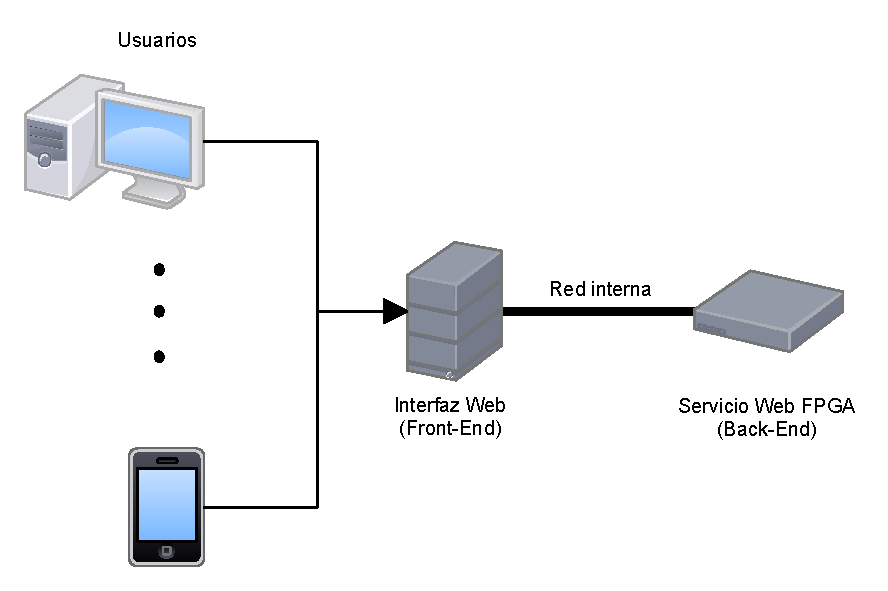
\includegraphics[width=0.7\textwidth,clip=true]{arquitectura}
  \caption{Arquitectura general de la aplicación.}
  \label{fig:arquitectura}
\end{figure}


\section{Back-End - Servicio Web FPGA\label{sec:dis:servicio_web_fpga}}

El componente \gls{back-end} se encarga de la interacción con la sonda de red (implementada en una \gls{FPGA}) y con el resto de partes involucradas en la reproducción y captura de tráfico de red.
Para ello, recibe peticiones \gls{HTTP} del \gls{front-end} (actuando en este caso como cliente), que se traducen en acciones sobre el sistema o en respuestas sobre el estado del mismo.
\begin{figure}[!htp]
  \centering
  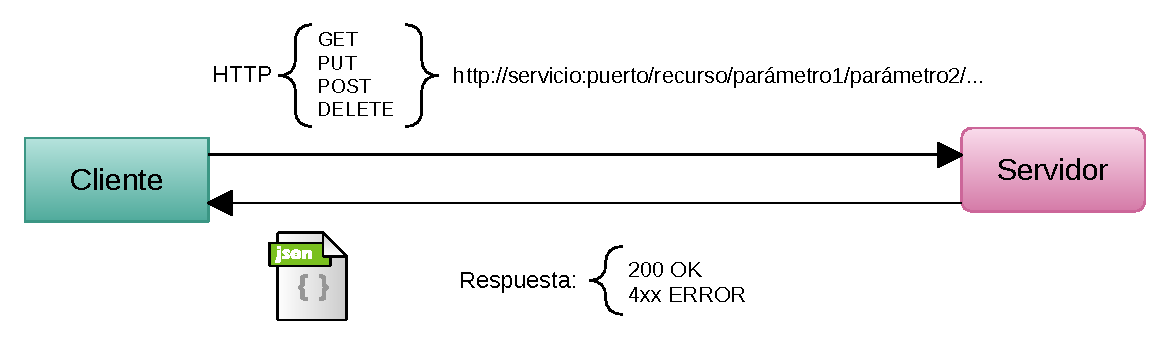
\includegraphics[width=0.95\textwidth,clip=true]{fpga_rest}
  \caption{Diagrama de flujo de un servicio \gls{REST}.}
  \label{fig:fpga_rest}
\end{figure}

La arquitectura de comunicación externa del \gls{back-end} se basa en el modelo de cliente-servidor \gls{REST} (ver Figura~\ref{fig:fpga_rest}).
Dentro de las directrices que marca este modelo, sólo se han considerado útiles para el problema dado un subconjunto de ellas:
\begin{itemize}
  \item El protocolo entre el cliente y el servidor debe ser sin estado: cada mensaje \gls{HTTP} tiene que contener toda la información necesaria para comprender la petición.
  \item Las operaciones se aplican sobre recursos mediante llamadas a métodos \gls{HTTP}: \textit{GET} para obtener información sobre un recurso, \textit{POST}/\textit{PUT} para actualizarlos o crearlos y \textit{DELETE} para borrarlos.
  \item Cada recurso debe tener un identificador único (en este caso, una \gls{URL} única).
\end{itemize}

Se ha decidido no adoptar el resto de directrices \gls{REST} debido a que no encajaban dentro del modelo de funcionamiento de la aplicación.
Así, no se facilita el descubrimiento automático de recursos y métodos, ya que se ha considerado que no tiene sentido siendo éste un subsistema interno y no un componente público.
Por otra parte, no se permiten distintas representaciones de un mismo recurso, siendo \gls{JSON} la única representación utilizada.
No seguir estas directrices simplifica además la implementación del \gls{back-end}.

\begin{figure}[!htp]
  \centering
  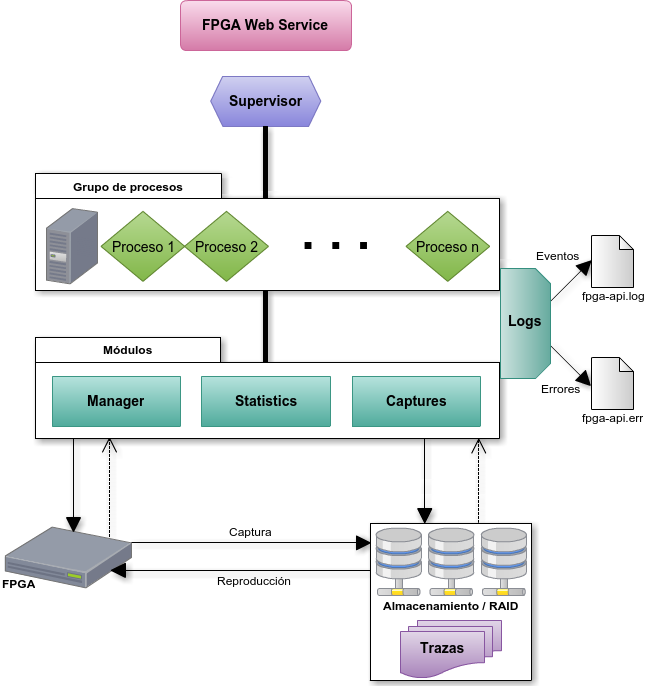
\includegraphics[width=0.95\textwidth,clip=true]{fpga}
  \caption{Arquitectura del \gls{servicioweb} \gls{FPGA}.}
  \label{fig:arquitectura_servicio}
\end{figure}

Internamente, el \gls{back-end} se estructura tal y como se describe en la Figura~\ref{fig:arquitectura_servicio}.
Un supervisor se encarga de vigilar al grupo de procesos que atienden las peticiones del \gls{front-end}, reemplazándolos en caso de que fallen.
Este grupo tiene tantos procesos como núcleos el servidor, adaptándose así a su arquitectura interna y consiguiendo por tanto una mayor disponibilidad y un menor tiempo de respuesta.
Por otro lado, con el objetivo de tener información detallada sobre el uso del servicio web, se registran todos los eventos y errores del \gls{back-end} en los \textit{logs} correspondientes.
Por último, se ha dividido el servicio web en tres módulos, cada uno con una funcialidad asociada: \textit{manager}, \textit{captures} y \textit{statistics}.

\subsection{Manager\label{ssec:dis:manager}}

Este módulo se encarga de gestionar el estado de la sonda de red y del servidor que la aloja.
Permite por tanto instalar, programar y montar la sonda en modo reproducción o en modo captura, ordenarle reproducir o capturar tráfico y pararla.
Adicionalmente, maneja también otros aspectos del sistema, posibilitando reiniciar el servidor y formatear el sistema de almacenamiento en caso de ser necesario.


\subsection{Captures\label{ssec:dis:captures}}

Este módulo se ocupa de todos los aspectos relacionados con las \glspl{traza} de tráfico de red.
Permite así listar todas las \gls{traza} disponibles, mostrando su nombre, fecha, tipo y tamaño.
Por otra parte, sobre una \gls{traza} concreta es capaz de detectar el formato interno de la misma, convertirla entre los formatos soportados, renombrarla o borrarla para liberar espacio de almacenamiento.


\subsection{Statistics\label{ssec:dis:statistics}}

Este módulo tiene como objetivo informar sobre el estado actual de la sonda de red, y proporcionar estadísticas sobre la reproducción o captura (en caso de existir una en curso).
Permite conocer además medidas sobre el almacenamiento: espacio ocupado, espacio disponible, velocidad de escritura global y por discos.


\section{Front-End - Interfaz web\label{sec:dis:interfaz_web}}

El \gls{front-end} se encarga de mostrar una interfaz web al usuario, recoger las acciones de éste y transformarlas en peticiones \gls{HTTP} al \gls{back-end}, informando de forma visual del resultado de la solicitud.
Este componente utiliza como punto de partida el \gls{framework} propio desarrollado (ver apéndice~\ref{extra:frameworkDesarrollado}).
Dicho \gls{framework} provee de una arquitectura y funcionalidad base a la interfaz, estructurando además los módulos de la misma siguiendo el patrón modelo-vista-controlador.

En el apartado visual, se ha decidido adoptar un diseño \textit{responsive}.
Esta filosofía de diseño se basa en la idea de que se debe adaptar la forma de mostrar una página para que la experiencia del usuario sea óptima independientemente del dispositivo que utilice (móvil, ordenador de sobremesa, etc.).
Para ello se utilizan una cuadrícula que cambia de posición y tamaño según sea el dispositivo desde el que se accede a la interfaz.
Ésta filosofía de diseño tiene una diferencia fundamental respecto al diseño \textit{adaptative}, que simplifica su implementación: mientras este último se basa en cargar distintos recursos de estilo según las características del dispositivo, el diseño \textit{responsive} utiliza una única cuadrícula que se ajusta en base a dichas características.

Respecto al idioma de la interfaz web, ésta estará disponible tanto en inglés como en español, pudiendo el usuario elegir el idioma que prefiera.
De forma similar, también se podrá seleccionar un tema visual para el \gls{front-end}.
Estos temas cambian el esquema de colores y aspectos menores de la interfaz gráfica.


\subsection{Maquetas\label{ssec:dis:maquetas}}

En este apartado se exponen las maquetas de las páginas principales de la interfaz, que sirven como guía para la implementación del \gls{front-end}.
Todas ellas cuentan con una barra superior de navegación, con enlaces al resto de pantallas principales de la interfaz.

En la Figura~\ref{fig:maqueta:configuracion} se muestra la maqueta de la pantalla de configuración de la aplicación.
En esta página se podrán configurar, mediante un formulario, la dirección del \gls{servicioweb} \gls{FPGA} (el \gls{back-end}), el idioma y el tema visual de la interfaz.
\begin{figure}[!htp]
  \centering
  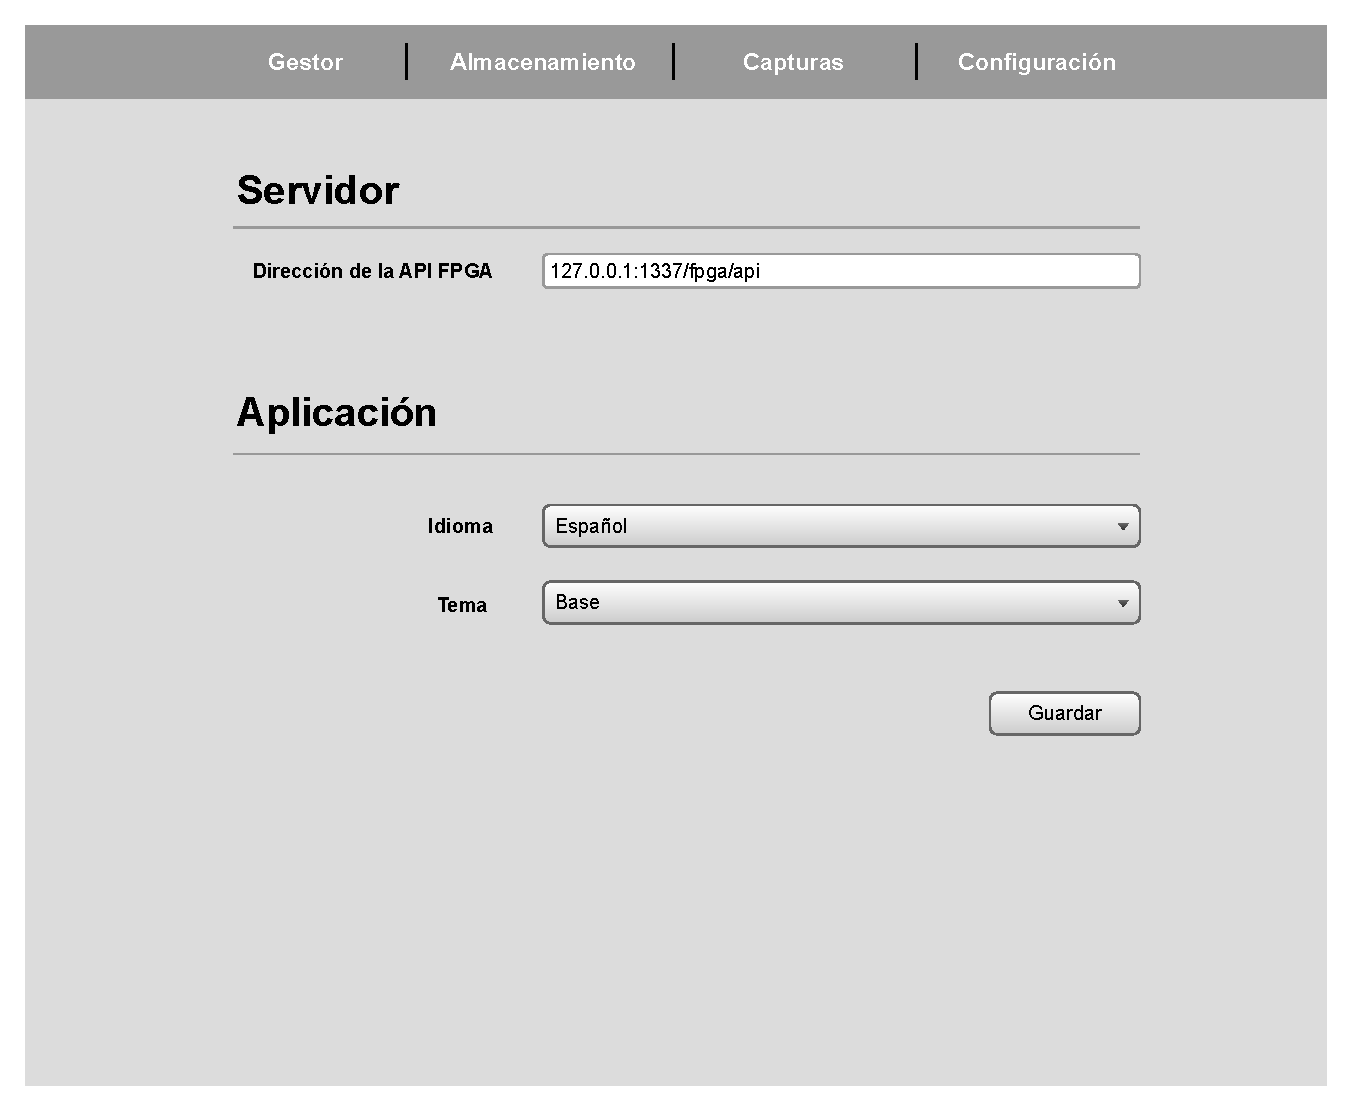
\includegraphics[width=\textwidth,clip=true]{maquetas/maqueta_configuracion}
  \caption{Maqueta de la pantalla de configuración de la aplicación.}
  \label{fig:maqueta:configuracion}
\end{figure}
\clearpage

En la Figura~\ref{fig:maqueta:almacenamiento} se muestra la maqueta de la pantalla de almacenamiento.
Esta página mostrará gráficas sobre el espacio disponible, y sobre estadísticas del \gls{RAID} en caso de estar configurado.
También se dará opción a formatear el \gls{RAID} en caso de que no tenga un rendimiento aceptable.
\begin{figure}[!htp]
  \centering
  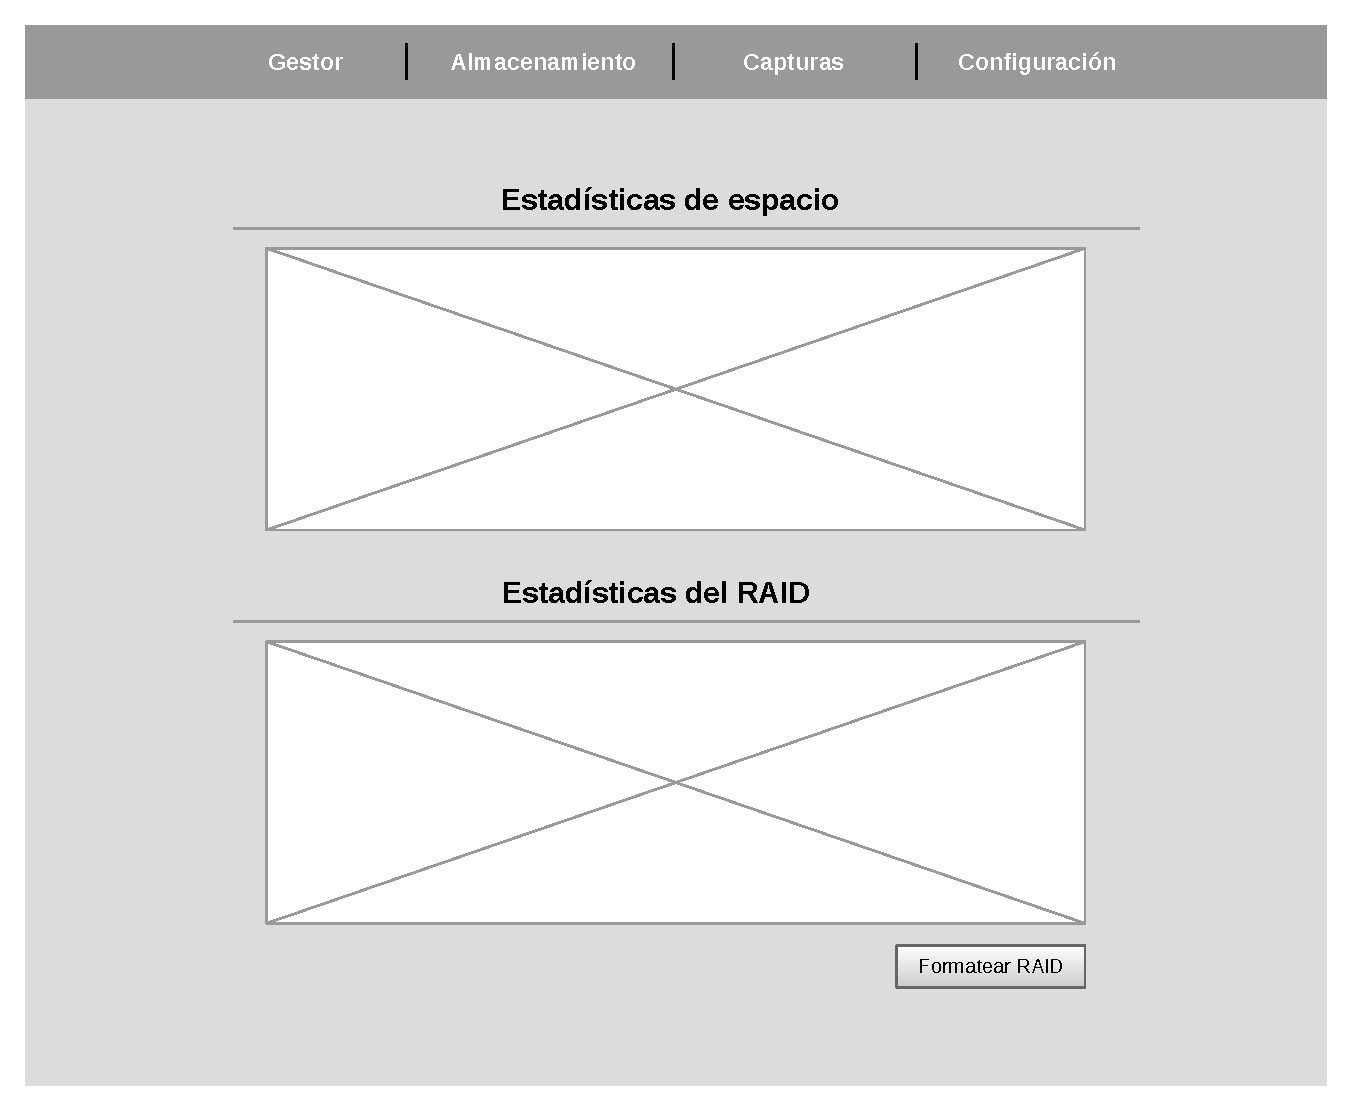
\includegraphics[width=\textwidth,clip=true]{maquetas/maqueta_almacenamiento}
  \caption{Maqueta de la pantalla de almacenamiento.}
  \label{fig:maqueta:almacenamiento}
\end{figure}
\clearpage

En la Figura~\ref{fig:maqueta:capturas} se muestra la maqueta de la pantalla de gestión de \glspl{traza}.
A la izquierda se podrán visualizar, en una tabla, todas las \glspl{traza} disponibles, con su nombre, tipo, tamaño y fecha.
Sobre esta tabla, una barra de acciones permitirá filtrar las \glspl{traza} según su tipo, o buscar alguna concreta por su nombre.
A la derecha se mostrará un panel con posibles acciones a realizar sobre la \gls{traza} seleccionada de la tabla: convertirla a otro formato, renombrarla o borrarla.
\begin{figure}[!htp]
  \centering
  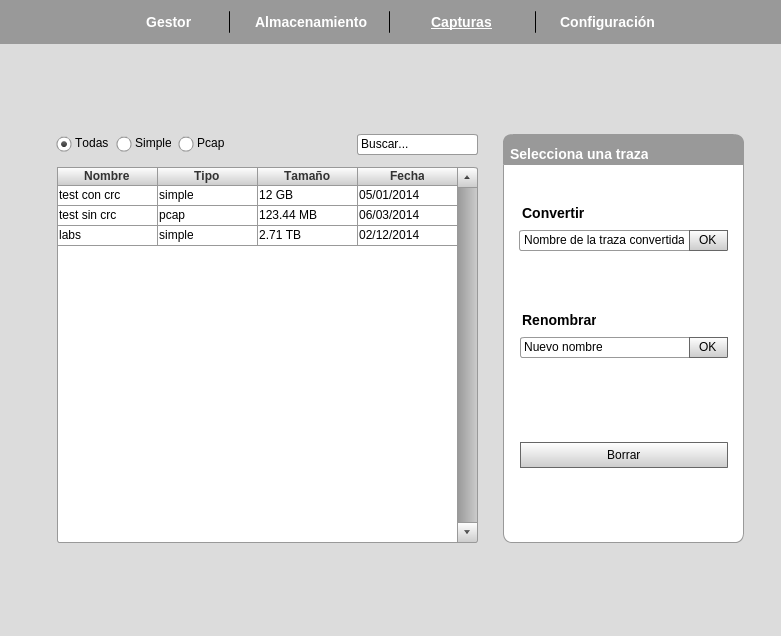
\includegraphics[width=\textwidth,clip=true]{maquetas/maqueta_capturas}
  \caption{Maqueta de la pantalla de gestión de \glspl{traza}.}
  \label{fig:maqueta:capturas}
\end{figure}
\clearpage

En la Figura~\ref{fig:maqueta:gestor_seleccion} se expone la maqueta de una de las pantallas de la página de gestión, que se mostrará en caso de que no se haya seleccionado aún ningún modo o cuando se quiera seleccionar otro.
Esta pantalla consta de dos botones, y pulsándo alguno se inicializará la sonda en el modo correspondiente.
\begin{figure}[!htp]
  \centering
  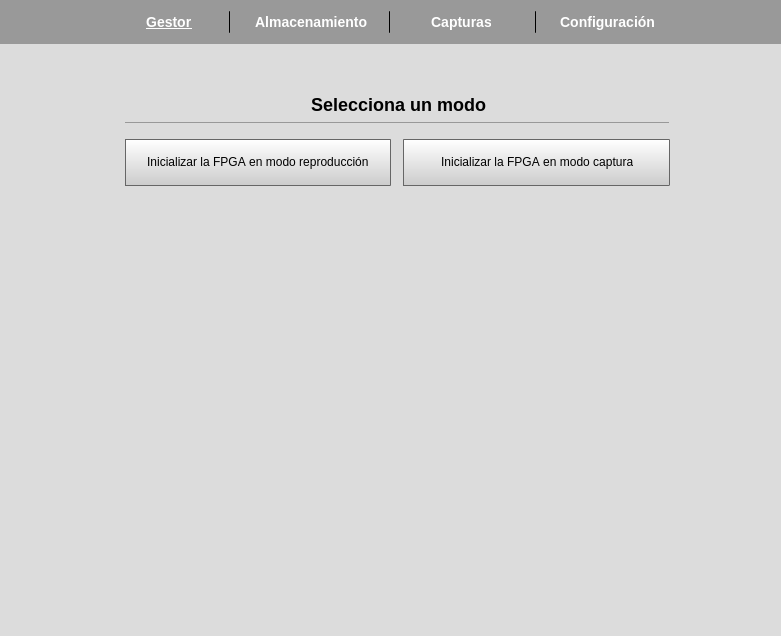
\includegraphics[width=\textwidth,clip=true]{maquetas/maqueta_gestor_seleccion}
  \caption{Maqueta de la pantalla de gestión - selección de modo.}
  \label{fig:maqueta:gestor_seleccion}
\end{figure}
\clearpage

En la Figura~\ref{fig:maqueta:gestor_capturador} se expone la maqueta de una de las pantallas de la página de gestión, que se mostrará cuando la sonda haya sido inicializada en modo captura.
En esta pantalla se podrá rellenar un formulario con el nombre de la \gls{traza} a capturar, su tamaño y el puerto del que capturar.
Pulsando el botón \textit{Capturar} se iniciará la captura de dicha \gls{traza}.
También se podrá volver a la página de selección de modo, pulsando el enlace inferior \textit{Cambiar de modo}.
\begin{figure}[!htp]
  \centering
  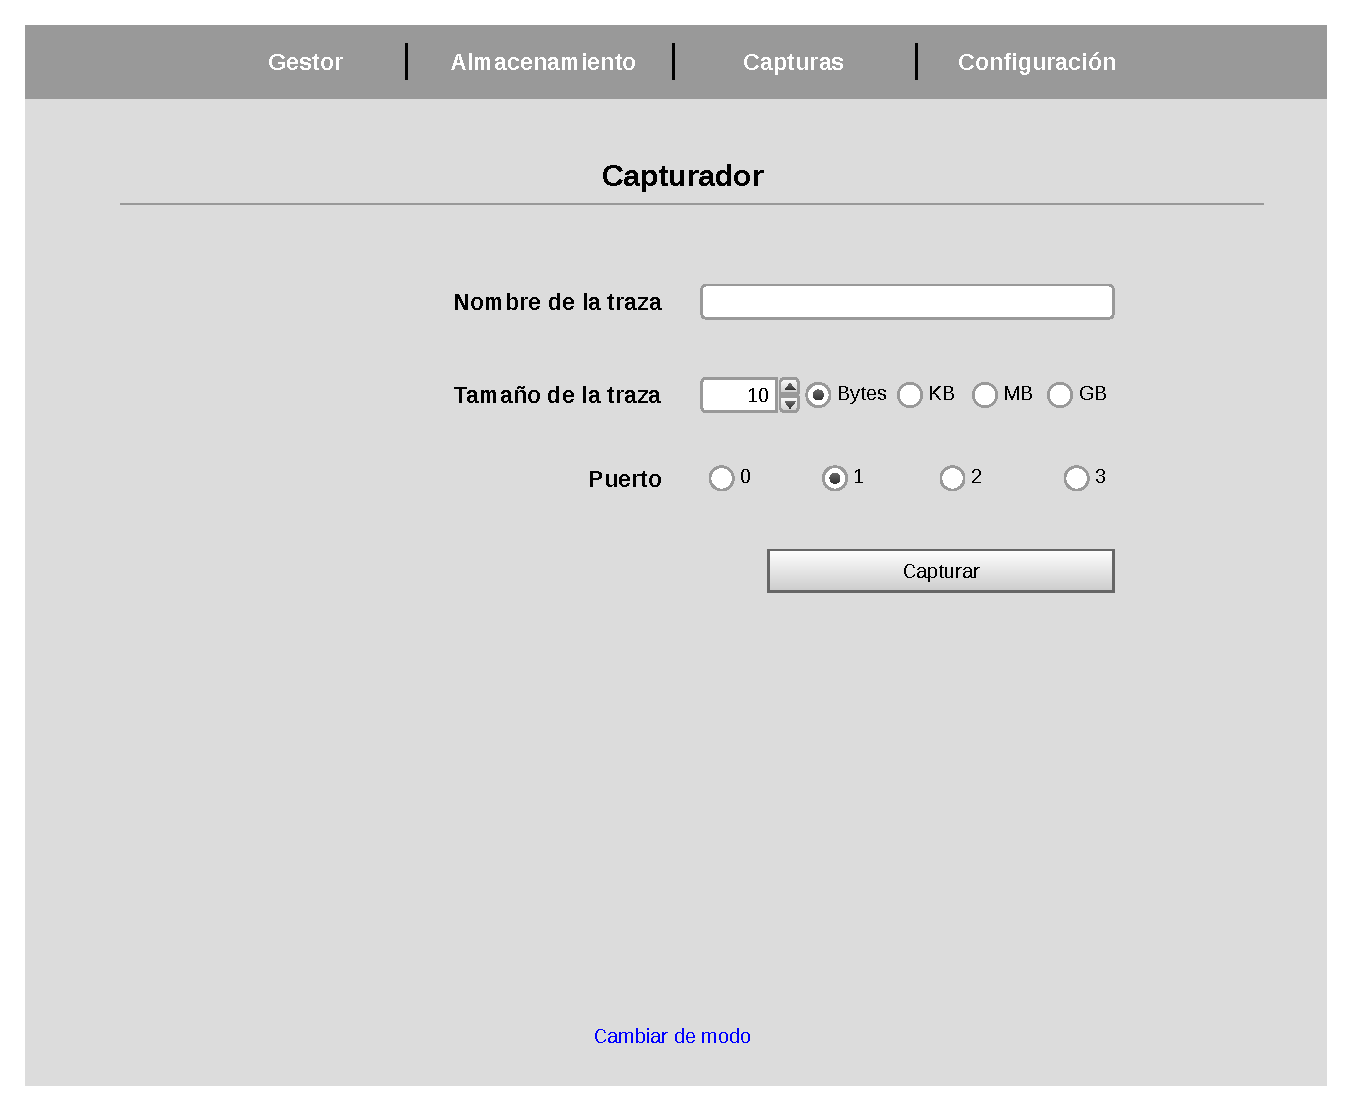
\includegraphics[width=\textwidth,clip=true]{maquetas/maqueta_gestor_capturador}
  \caption{Maqueta de la pantalla de gestión - formulario para capturar.}
  \label{fig:maqueta:gestor_capturador}
\end{figure}
\clearpage

En la Figura~\ref{fig:maqueta:gestor_capturando} se expone la maqueta de otra de las pantallas de gestión, que se mostrará cuando la sonda esté capturando tráfico de red.
En esta pantalla se podrán visualizar distintas estadísticas de la captura en curso, hasta que ésta finalice.
Adicionalmente, una barra de progreso indicará qué porcentaje de la \gls{traza} ha sido ya capturado.
También se podrá parar la captura, pulsando el botón \textit{Detener la captura}.
\begin{figure}[!htp]
  \centering
  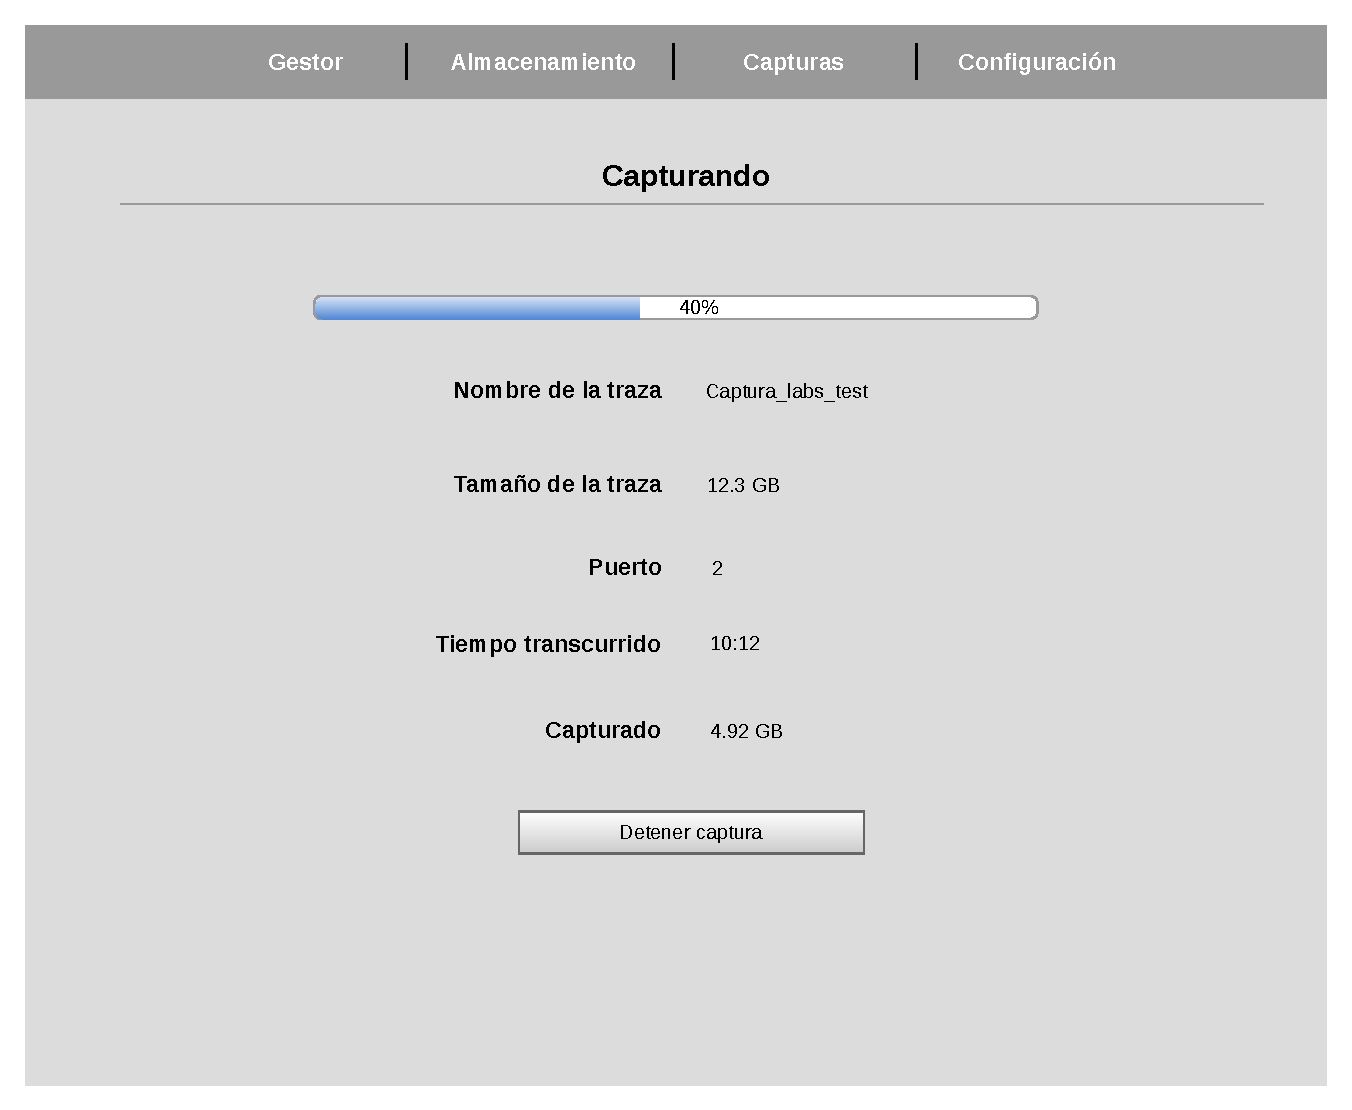
\includegraphics[width=\textwidth,clip=true]{maquetas/maqueta_gestor_capturando}
  \caption{Maqueta de la pantalla de gestión - capturando.}
  \label{fig:maqueta:gestor_capturando}
\end{figure}
\clearpage

En la Figura~\ref{fig:maqueta:gestor_reproductor} se expone la maqueta de otra de las pantallas de la página de gestión, que se mostrará cuando la sonda haya sido inicializada en modo reproducción.
A la izquierda se podrán visualizar, en una tabla, todas las \glspl{traza} disponibles para reproducir, con su nombre, tipo, tamaño y fecha.
Sobre esta tabla, una barra de acciones permitirá filtrar las \glspl{traza} según su tipo, o buscar alguna concreta por su nombre.
A la derecha se mostrará un panel con un formulario para configurar las opciones de reproducción: en bucle o no, \gls{IFG} y máscara de reproducción.
Pulsando el botón \textit{Reproducir} se iniciará la reproducción de la traza seleccionada.
También se podrá volver a la página de selección de modo, pulsando el enlace inferior \textit{Cambiar de modo}.
\begin{figure}[!htp]
  \centering
  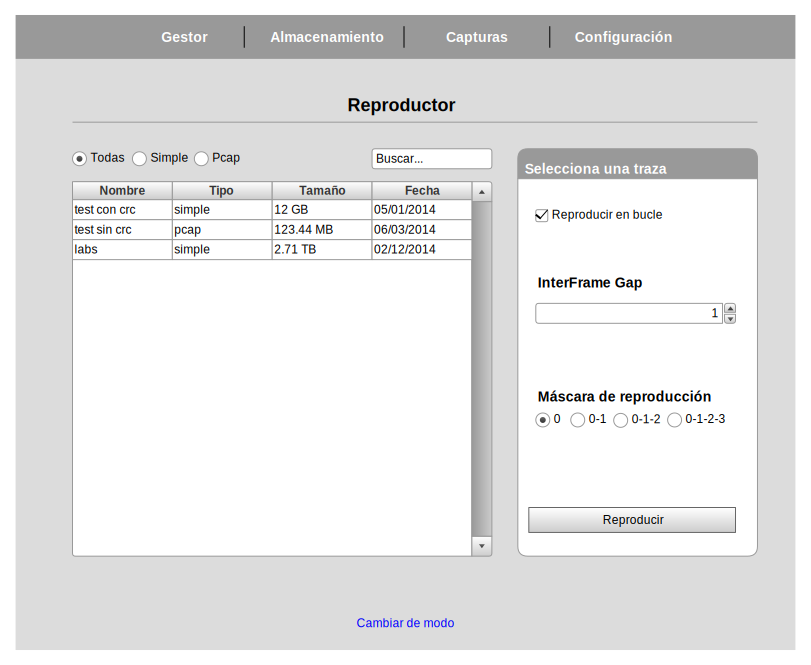
\includegraphics[width=\textwidth,clip=true]{maquetas/maqueta_gestor_reproductor}
  \caption{Maqueta de la pantalla de gestión - formulario para reproducir.}
  \label{fig:maqueta:gestor_reproductor}
\end{figure}
\clearpage

En la Figura~\ref{fig:maqueta:gestor_reproduciendo} se expone la maqueta de otra de las pantallas de gestión, que se mostrará cuando la sonda esté reproduciendo una \gls{traza}.
En esta pantalla se podrán visualizar distintas estadísticas de la reproducción en curso, hasta que ésta finalice.
También se podrá parar la reproducción, pulsando el botón \textit{Detener la reproducción}.
\begin{figure}[!htp]
  \centering
  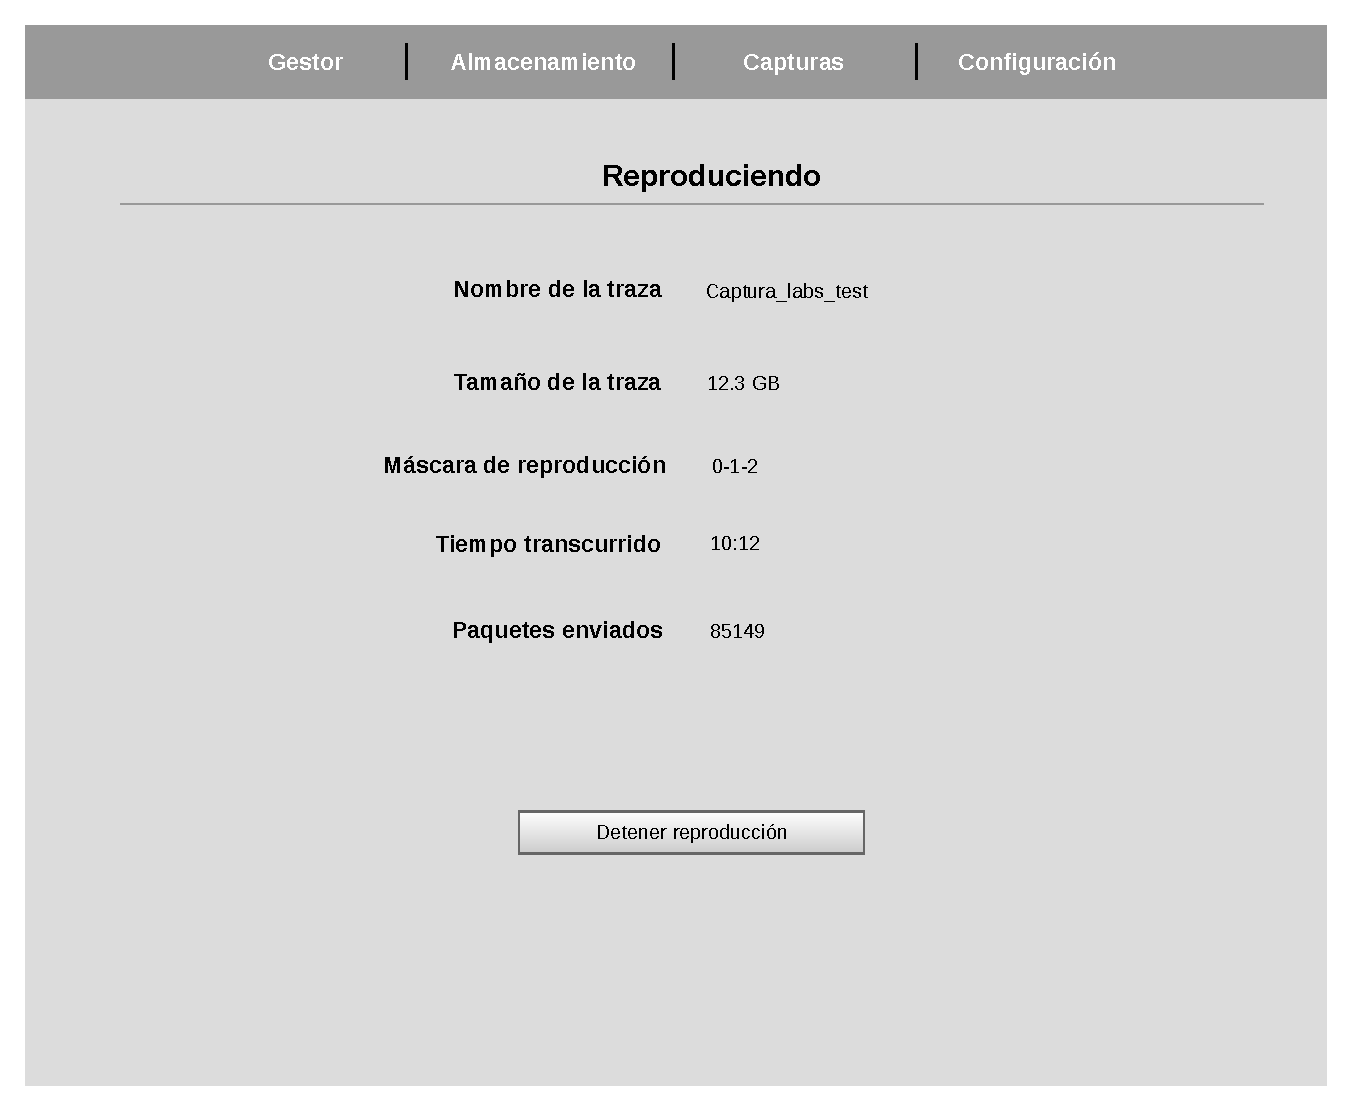
\includegraphics[width=\textwidth,clip=true]{maquetas/maqueta_gestor_reproduciendo}
  \caption{Maqueta de la pantalla de gestión - reproduciendo.}
  \label{fig:maqueta:gestor_reproduciendo}
\end{figure}
\chapter{Implementación\label{cap:implementacion}}

En este capítulo se explica cómo se han implementado los dos componentes principales de la aplicación: el \gls{back-end} y el \gls{front-end}, tal y como se diseñaron y estructuraron en el capítulo \ref{cap:disenho}.
Se detalla además la documentación generada, tanto interna como para el usuario final.

\section{Back-End\label{sec:imp:back_end}}

Para la implementación del \gls{back-end} se han utilizado las librerías mencionadas en la sección \ref{ssec:dp:back-end}.
Se ha encapsulado este componente en un servicio que se inicia automáticamente al arrancar el ordenador.
Esto permite que el \gls{back-end} esté activo siempre que el servidor de la sonda de red esté operativo.

\begin{figure}[!htp]
  \centering
  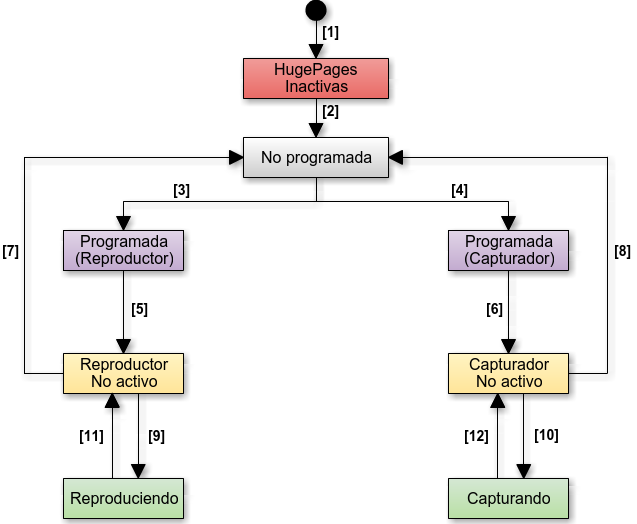
\includegraphics[width=\textwidth,clip=true]{fpga_estado}
  \caption{Máquina de Estados Finitos del \gls{back-end}.}
  \label{fig:fpga_estado}
\end{figure}

El objetivo principal del \gls{back-end} es formalizar el estado de la \gls{FPGA}, permitiendo así su consulta y modificación.
Para programar este aspecto, se han formalizado los posibles estados internos del sistema en una Máquina de Estados Finitos (ver Figura~\ref{fig:fpga_estado}).
Las transiciones existentes entre los estados son:
\begin{enumerate}[label={\bfseries [\arabic*]}]
  \item Iniciar el servidor sin seleccionar la opción de arrancar con \textit{HugePages} habilitadas.
  \item Reiniciar el servidor, seleccionando la opción de arrancar con \textit{HugePages} habilitadas.
  \item Programar la \gls{FPGA} en modo reproductor con el \gls{bitstream} correspondiente y reiniciar el servidor.
  \item Programar la \gls{FPGA} en modo capturador con el \gls{bitstream} correspondiente y reiniciar el servidor.
  \item Montar la \gls{FPGA} sobre el servidor.
  \item Montar la \gls{FPGA} sobre el servidor.
  \item Reiniciar el servidor.
  \item Reiniciar el servidor.
  \item Ordenar a la sonda reproducir una \gls{traza}.
  \item Ordenar a la sonda capturar una \gls{traza}.
  \item Reproducción finalizada, o porque se ha acabado el contenido de la \gls{traza} o porque ha sido detenida el usuario.
  \item Captura finalizada, o porque se ha capturado todo lo que se quería o porque es detenida por el usuario.
\end{enumerate}

Para conocer el estado actual de esta máquina de estados y verificar qué operaciones puede realizar la \gls{FPGA}, se plantearon dos opciones: mantener sincronizadas la sonda de red y el servicio web, de forma que el se detectase cualquier cambio en la \gls{FPGA} y el servicio web almacenase el estado de forma persistente, o que cada vez que se necesitase conocer el estado de la sonda se determinase de nuevo.
Se ha elegido la segunda opción, ya que evita que pueda haber incoherencias entre el estado real de la \gls{FPGA} y el guardado en el servicio.
Además, así el servicio web tendrá que consultar a la sonda solo en caso de que haya una petición dirigida al \gls{back-end}, no utilizando recursos monitorizando la \gls{FPGA} si no ha sido invocado.
Se ha implementado, siguiendo esta segunda opción, un árbol de decisión binario que determina el estado actual de la \gls{FPGA} mediante consultas a la propia sonda y al sistema (ver Figura~\ref{fig:arbol_decision}).

\begin{figure}[!htp]
  \centering
  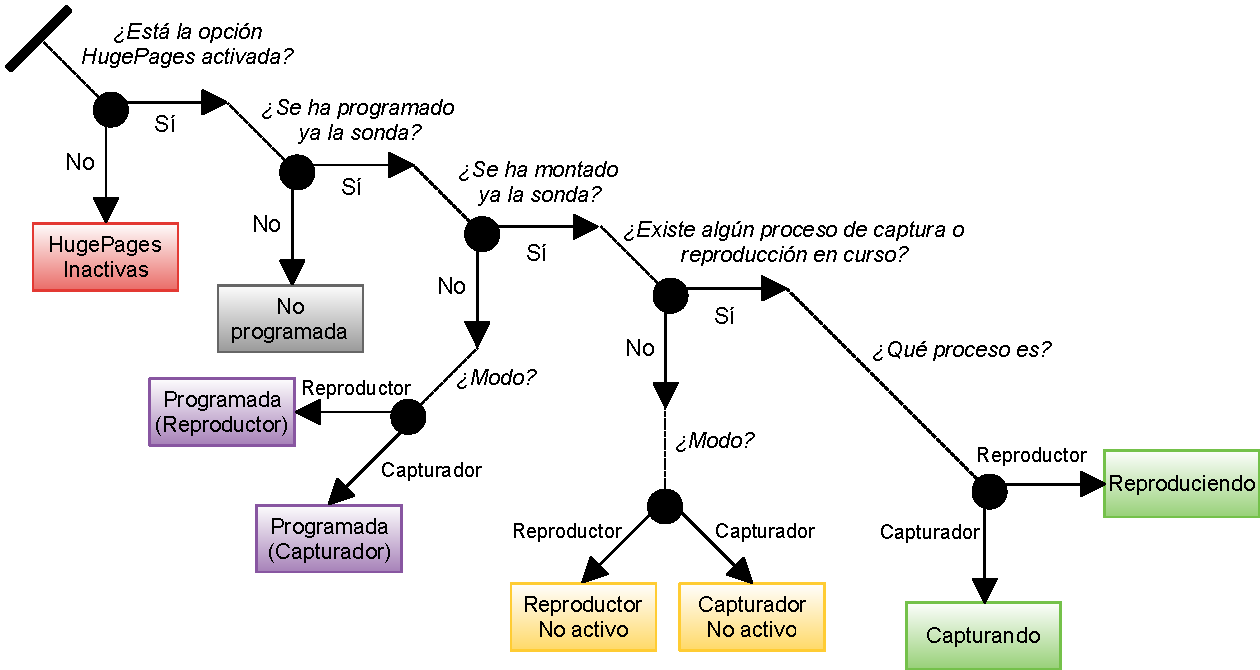
\includegraphics[width=0.75\textwidth,clip=true]{arbol_decision}
  \caption{Árbol de decisión para determinar el estado de la \gls{FPGA}.}
  \label{fig:arbol_decision}
\end{figure}

Los archivos de código más relevantes de la implementación del \gls{back-end} se muestran en la Figura~\ref{fig:arbol_codigo}, siendo \textit{server.js} el principal. Este se encarga de lanzar el grupo de procesos que responde a las peticiones del \gls{front-end}, delegándolas según corresponda a uno de los tres módulos existentes.
Cada uno de estos módulos consta de dos archivos en \textit{JavaScript}.
El primero, con el nombre del propio módulo, contiene las funciones de la \gls{API} del \gls{back-end} (ver Figura~\ref{fig:arbol_metodos}).
El segundo fichero, con el nombre del módulo seguido de \textit{\_utils}, recoge funciones auxiliares.
Por último, las funciones comunes a todos los módulos han sido codificadas en un único archivo, \textit{\_common.js}.

\begin{figure}[!htp]
  \begin{center}
    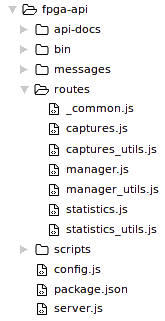
\includegraphics[width=0.3\textwidth,clip=true]{capturas/arbol_backend}
    \hspace{1cm}
    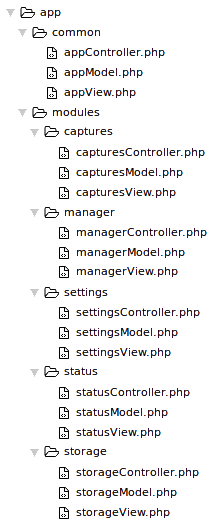
\includegraphics[width=0.3\textwidth,clip=true]{capturas/arbol_frontend}
  \caption{Árboles con los principales archivos de código del \gls{back-end} (a la izquierda) y del \gls{front-end} (a la derecha).}
  \label{fig:arbol_codigo}
  \end{center}
\end{figure}

\begin{figure}[!htp]
  \centering
  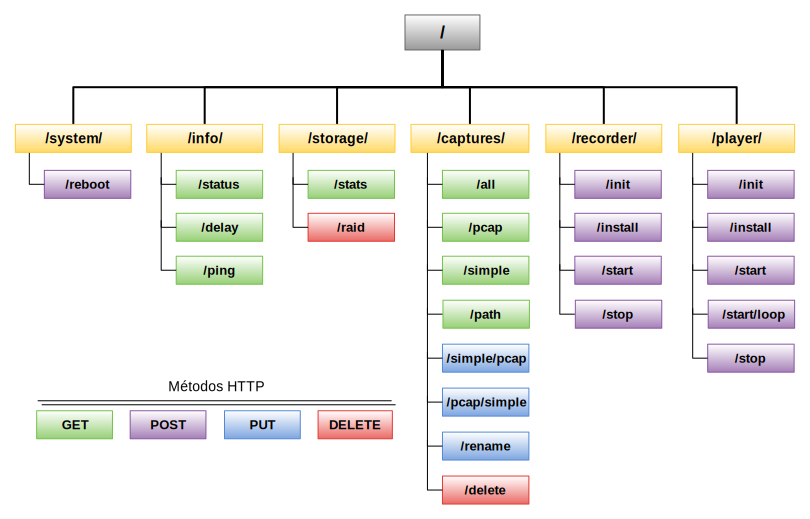
\includegraphics[width=\textwidth,clip=true]{arbol_metodos}
  \caption{Métodos públicos del \gls{servicioweb} \gls{FPGA}.}
  \label{fig:arbol_metodos}
\end{figure}

\section{Front-End\label{sec:imp:front_end}}

Introducción, se ha utilizadon utilizado las herramientas descritas en ref

Notificaciones como respuesta a acciones menores > cambio de páginas para mayores

Internacionalización, inglés y español

Resultado Capturas diseño responsive,  (misma página desde dos sitios)~\ref{fig:captura:movil}
\begin{figure}[!htp]
  \centering
  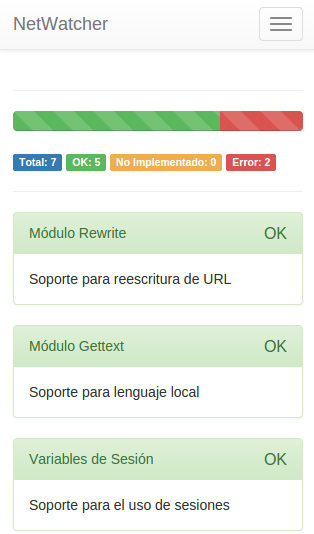
\includegraphics[width=0.4\textwidth,clip=true]{capturas/estado_movil}
  \caption{Página de la aplicación visualizada desde un dispositivo móvil.}
  \label{fig:captura:movil}
\end{figure}

Temas (captura algún temas)~\ref{fig:captura:oscuro}
\begin{figure}[!htp]
  \centering
  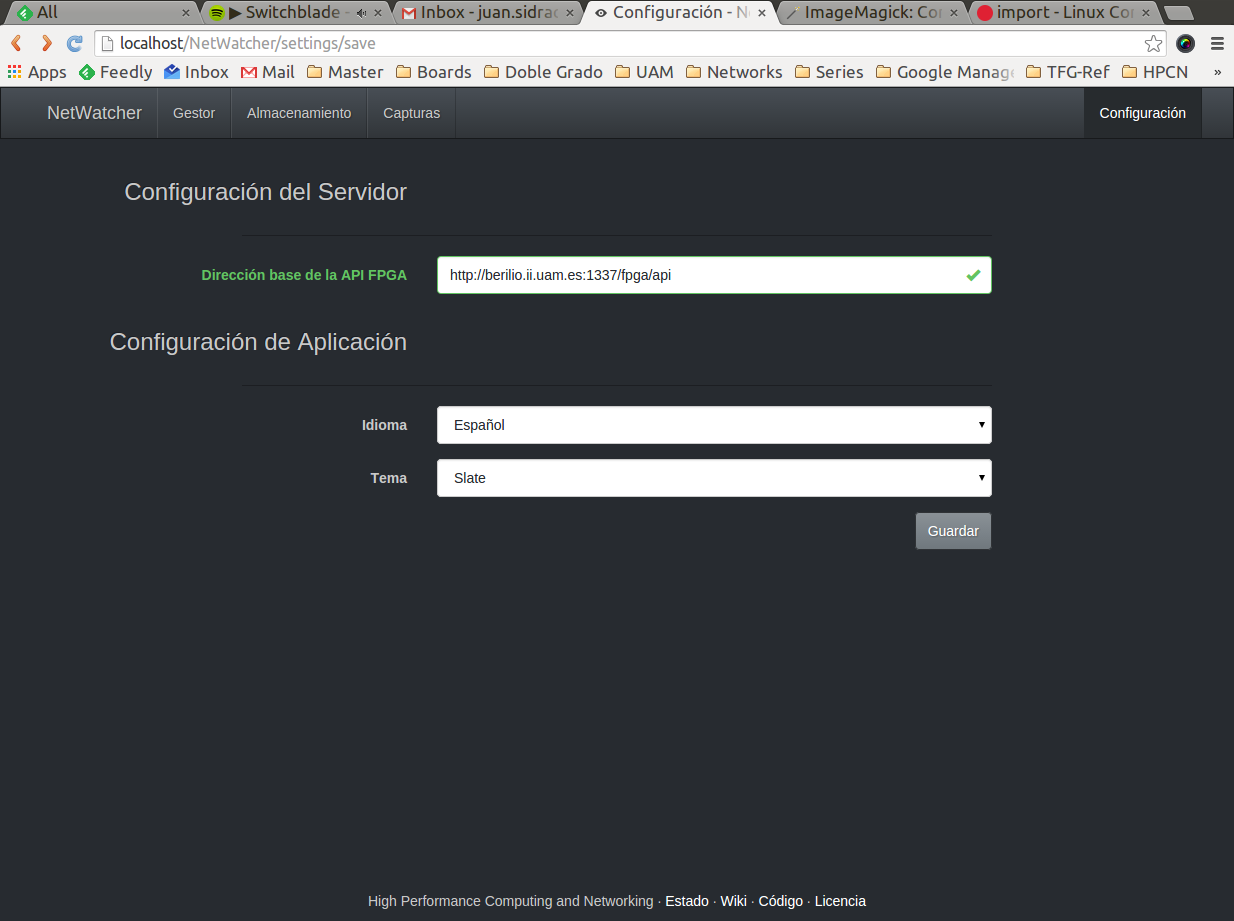
\includegraphics[width=0.95\textwidth,clip=true]{capturas/configuracion_tema_oscuro}
  \caption{Página de la aplicación con un tema oscuro seleccionado.}
  \label{fig:captura:oscuro}
\end{figure}

Captura árbol de archivos~\ref{fig:arbol_codigo}, cada módulo hereda y sobreescribe MVC

\section{Documentación \label{sec:imp:docs}}

Se ha creado distinta documentación del proyecto según a quién esté dirigida.
Por un lado, se ha escrito un manual de usuario (disponible en el apéndice~\ref{extra:manual_de_usuario}), que pretende ser una guía completa y suficiente para la instalación, configuración y uso de la aplicación.
Adicionalmente, se han publicado en el repositorio de \textit{GitHub} del proyecto (\url{github.com/JSidrach/NetWatcher}) una serie de páginas en formato \textit{wiki} (ver Figura~\ref{fig:captura:wiki}). Estas páginas, en inglés, recogen los aspectos más importantes de la aplicación, tanto para el usuario final como para desarrolladores.

\begin{figure}[!htp]
  \centering
  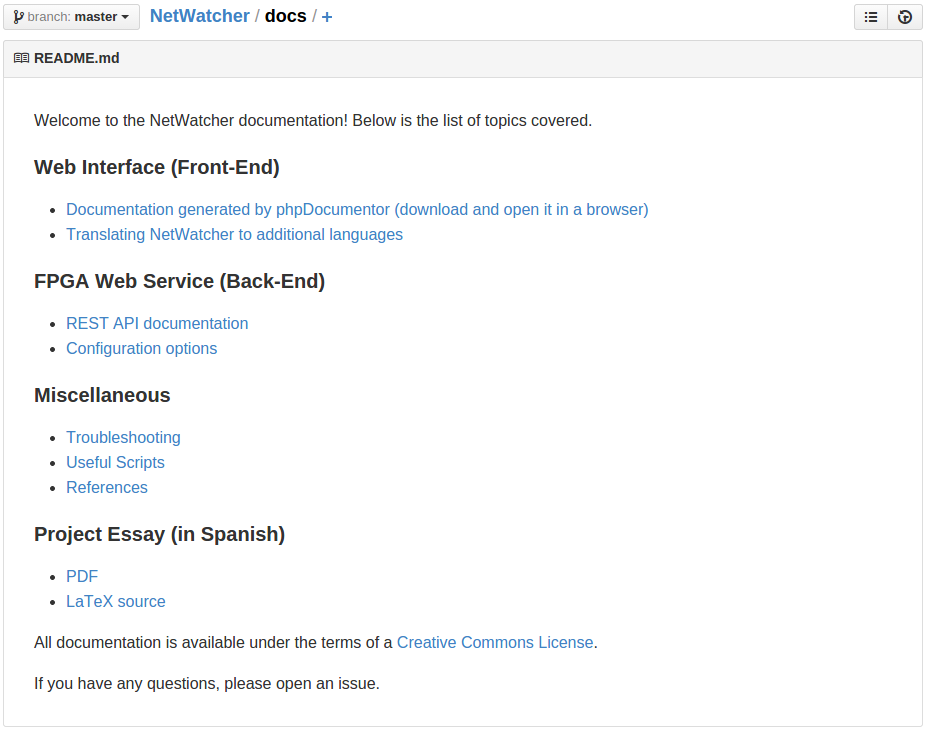
\includegraphics[width=0.95\textwidth,clip=true]{graphics/capturas/github_docs}
  \caption{Captura de una de las páginas de la wiki del proyecto.}
  \label{fig:captura:wiki}
\end{figure}

A nivel específico de desarrollador, se han utilizado dos herramientas para crear la documentación interna, accesible a través del navegador y en inglés.
La documentación del \gls{front-end} se ha generado con \textit{phpDocumentor} (ver Figura~\ref{fig:captura:docsfrontend}), y la del \gls{back-end} con \textit{apiDoc}.
Esta última se adjunta también, traducida al español, en el apéndice~\ref{extra:api_servicio_web_fpga}.
Por último, en el apéndice~\ref{extra:frameworkDesarrollado} se explican la arquitectura y funcionalidad del \gls{framework} base para el \gls{front-end}.

\begin{figure}[!htp]
  \centering
  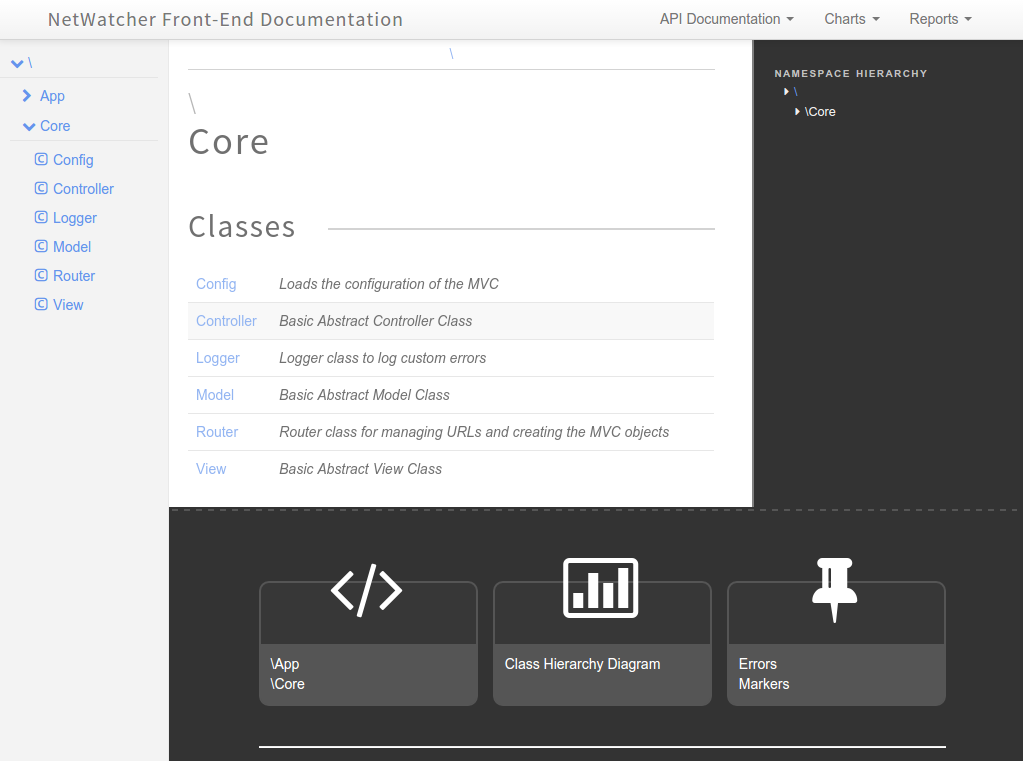
\includegraphics[width=0.95\textwidth,clip=true]{graphics/capturas/docs_frontend}
  \caption{Documentación web del \gls{front-end}.}
  \label{fig:captura:docsfrontend}
\end{figure}

\chapter{Pruebas\label{cap:pruebas}}

TODO: [Introducción]
- Por qué han sido importantes
- Quién las ha realizado
  - Estudiante
    - Otros miembros del grupo de investigación (potenciales usuarios)
- División entre pruebas de verificación y pruebas de validación

\section{Pruebas de verificación\label{sec:pb:verificacion}}

TODO: Pruebas de verificación
- Qué son
- Plan de pruebas: todas las pruebas que se han realizado
- Tipos de pruebas

\subsection*{Inspección del código\label{ssec:pb:inspeccion}}

La inspección del código es una técnica que consiste en revisar el código fuente.
Se ha aplicado en todos los archivos de código del proyecto, con el objetivo mejorar la estructura interna y el estilo del código fuente.
Sin embargo, no se ha utilizado para descubrir errores, ya que para eso se ha recurrido a otro tipo de pruebas, como las de caja negra y las de caja blanca.

La estrategia seguida ha sido realizar una inspección en cada fichero, una vez ha pasado al menos una semana desde su codificación.
Así, al no tenerla tan cercana, se ha facilitado el evaluar de manera más objetiva la implementación.
Como consecuencia de estas inspecciones, se ha refactorizado parte del código, mejorando su estructura interna, claridad y mantenibilidad.

\subsection*{Pruebas de caja blanca\label{ssec:pb:caja_blanca}}

Las pruebas de caja blanca son las que se realizan teniendo en cuenta la estructura interna del programa.
Tienen como objetivo verificar el correcto funcionamiento del código y detectar errores.
Concretamente, se han llevado a cabo aquellas basadas en la comprobación de los posibles flujos de ejecución de una función, mediante su invocación con valores típicos, aleatorios y límites.

Debido al alto coste temporal de plantear y ejecutar este tipo de pruebas para todo el sistema, se ha decidido aplicarlas en un único submódulo, considerado crítico para la aplicación: la máquina de estados finitos que formaliza el estado de la \gls{FPGA}.
Como resultado de estas pruebas, se han corregido errores menores que se producían en su mayoría con valores extremos.

\subsection*{Pruebas de caja negra\label{ssec:pb:caja_negra}}

Las pruebas de caja negra, en contraposición con las de caja blanca, son aquellas que se realizan sin tener conocimiento de la estructura interna del programa.
Se ha utilizado este tipo de pruebas
Estas pruebas la ejecución
pruebas de caja blanca
    Estrategia ascendente, separando back-end y front-end
Back-End
unitarias
common > utils > funciones de la API (POSTMAN)
    - Fácilmente replicables, test de pruebas exportado/importable a la app
        - Postman, cada uno de los métodos de la API pública del back-end, que hacían uso de los métodos básicos
Front-End
    - Proxy
    - Modelo MVC

    Resultado


\subsection*{Pruebas de integración\label{ssec:pb:integracion}}
  - Prueba de integración
    Back-end y front-end
    Resultado

\subsection*{Pruebas sobre la interfaz de usuario\label{ssec:pb:interfaz}}

    - para cualquier estado de la sonda
    - cambios esperados en la interfaz
    - valores límite en los formularios disponibles

\section{Pruebas de validación\label{sec:pb:validacion}}

TODO: Pruebas de validación
- Qué son

- Comprobación de los requisitos
  - Se cumplen todos los funcionales, cómo se comprueba
  - Se cumplen todos los no funcionales, cómo se comprueban

\chapter{Mantenimiento\label{cap:mantenimiento}}

Se expone a continuación el plan de mantenimiento para la aplicación desarrollada.
Dentro de las diferentes categorías de mantenimiento (perfectivo, adaptativo, preventivo y correctivo), solo entra dentro del alcance de este proyecto realizar un mantenimiento correctivo hasta máximo un mes después de entregar el producto final (al menos por parte del estudiante).
Esta decisión ha sido fundamentada en el límite de tiempo que se recomienda para la elaboración del Trabajo de Fin de Grado.
Se diagnosticarán y corregirán por tanto errores durante el periodo establecido, como respuesta a solicitudes de los usuarios (a través de la apertura de peticiones en el repositorio del código).

Se han identificado, no obstante, líneas de trabajo futuro y posibles mejoras (ver capítulo~\ref{cap:lineasDeTrabajoFuturo}) que no entrarían dentro de este tipo de mantenimiento, pero cuyo planteamiento se ha considerado interesante.
Por ello, se ha decidido liberar el código de la aplicación en \textit{GitHub} (\url{https://github.com/JSidrach/NetWatcher}) bajo la licencia \textit{MIT} \cite{mit}, de forma que el proyecto pueda ser continuado por otras personas.
Se ha seleccionado \textit{GitHub} como plataforma para alojar el código porque facilita la colaboración entre desarrolladores y porque el propio proyecto ya estaba alojado allí de manera privada, no requiriéndose una migración.
Se ha elegido la licencia \textit{MIT} por ser una de las menos restrictivas dentro de las de código abierto~\cite{licenses}, permitiendo que cualquiera pueda utilizar y modificar la aplicación siempre que se reconozca la autoría original.
Se espera así que en un futuro otras personas puedan ampliar el trabajo realizado.

\chapter{Conclusiones\label{cap:conclusiones}}

Este Trabajo de Fin de Grado ha consistido en el desarrollo de una interfaz para la gestión de sondas de red de altas prestaciones.
Para ello, se ha analizado el problema, estudiado el estado del arte, definido de forma rigurosa y completa el proyecto a realizar, diseñado la solución, implementado la misma, llevado a cabo una verificación y validación del sistema y, por último, se ha ejecutado un mantenimiento correctivo.

La aplicación propuesta facilita la utilización de la sonda de red mediante una interfaz gráfica basada en tecnologías web.
Esta interfaz puede ser utilizada por cualquier usuario con conocimientos informáticos, sin ser necesario un conocimiento específico de la sonda en sí.
Se cumple así el objetivo de simplificar el empleo de la sonda seleccionada que anteriormente solo se podía manejar por línea de comandos.
También agrupa otros aspectos relevantes de la captura y reproducción de tráfico web, como la gestión del almacenamiento de las \glspl{traza}, la velocidad de escritura en disco o la conversión entre formatos de \gls{traza}.
La implementación de la interfaz sigue un diseño \textit{responsive}, lo que hace que se pueda utilizar desde dispositivos móviles sin empeorar la experiencia de usuario.
Se ha conseguido, como producto final, una interfaz elegante que permite gestionar todos los aspectos de la sonda considerados relevantes, presentando el estado e información adicional del sistema de forma visual, mediante gráficos y estadísticas.

Sin embargo, este proyecto no ha consistido únicamente en el desarrollo de una interfaz.
Se ha dividido el sistema en dos componentes, \gls{back-end} y \gls{front-end}, que se comunican entre sí y que pueden estar alojados en un servidor distinto cada uno.
Así, se ha diseñado e implementado un \gls{servicioweb} \gls{REST} en el \gls{back-end}, que formaliza el estado y funcionalidad de la \gls{FPGA}, añadiendo también control sobre otros aspectos relevantes mencionados anteriormente.
Para el \gls{front-end}, se ha creado un \gls{framework} propio, sobre el que se ha implementado la interfaz web.
Esta arquitectura de la aplicación cuenta con ciertas ventajas respecto a no separar físicamente el \gls{front-end} y el \gls{back-end}.
Al monitorizar el estado de la \gls{FPGA}, la interfaz estará disponible aunque el servidor que aloja la sonda no se encuentre operativo.
Por otra parte, al trasladar la interfaz a un servidor distinto, se libera parte de los recursos del servidor conectado a la sonda de red, afectando menos a su rendimiento.
Este proyecto, por tanto, proporciona una base sólida sobre la que se puede incluir soporte a otras sondas de red sin partir desde cero, y siendo solo necesario modificar una parte bien diferenciada del \gls{back-end}.

Para la implementación de la aplicación, se han utilizado diversos lenguajes de programación y herramientas, lo que constituye, sin duda, una valiosa experiencia para el futuro profesional del estudiante.
En el \gls{back-end} se ha empleado \textit{node.js}, una librería para construir aplicaciones de red en \textit{JavaScript} (tradicionalmente utilizado en el cliente, no en el servidor).
La codificación sobre esta librería se basa en la programación asíncrona, paradigma que ha sido enriquecedor aprender.
El \gls{front-end} se ha implementado con varios lenguajes de programación: \textit{PHP}, \textit{JavaScript}, \textit{HTML} y \textit{CSS}.
Se han empleado en este componente las librerías \textit{Bootstrap} y \textit{jQuery}, comunes en el desarrollo de páginas web.

Durante el desarrollo de este proyecto, se han podido poner en práctica conocimientos adquiridos en diversas asignaturas del Grado en Ingeniería Informática.
Por ejemplo, se ha seguido un proceso completo de desarrollo \textit{software}, aprendido en Ingeniería del Software.
Asignaturas como Arquitectura de Computadores y Redes de Comunicación han sido claves, al ser el trabajo base del que parte este proyecto una sonda de red (que a pesar de no haberse modificado, sí ha sido necesario entender su funcionamiento).
Conceptos como \gls{servicioweb}, \gls{API} \gls{REST} y algunos lenguajes de programación web fueron estudiados en Sistemas Informáticos I y II, lo que ha agilizado su adopción.

Por último, destacar que se ha liberado el código fuente del proyecto en la plataforma \textit{GitHub} (\url{https://github.com/JSidrach/NetWatcher}).
Esto no ha sido un simple gesto, ya que se ha invertido tiempo adicional en documentar todo el código de la aplicación en inglés.
Además, se han creado páginas \textit{wiki} dentro de la propia plataforma explicando el funcionamiento interno de la aplicación, junto con manuales de instalación, configuración, etc.
Se espera, con este esfuerzo, fomentar la participación de otros desarrolladores de la comunidad en la ampliación y mejora del sistema implementado (se dan algunas ideas en el capítulo~\ref{cap:lineasDeTrabajoFuturo}).
Liberar el proyecto ha consistido también en mejorar y poner a disposición de otros alumnos la plantilla en \textit{LaTeX} creada para esta memoria, que se encuentra disponible en otro repositorio público de \textit{GitHub} (\url{https://github.com/JSidrach/tfg-plantilla}).
A fecha de hoy, esta plantilla está siendo utilizada en varios trabajos más.

\chapter{Líneas de trabajo futuro\label{cap:lineasDeTrabajoFuturo}}

En el contexto de este Trabajo de Fin de Grado, se ha desarrollado una interfaz web para el manejo de sondas red de altas prestaciones. Gracias al trabajo realizado, se han identificado áreas de interés que podrían ser consideradas con el objetivo de mejorar y ampliar la aplicación en el futuro, y que no han podido ser abordadas en el mismo por la limitación del tiempo disponible. Se describen a continuación algunas de estas posibles mejoras.

\subsection*{Estandarización del Servicio Web}

La aplicación implementada gestiona un dispositivo concreto de captura y reproducción de tráfico de red. Aunque algunos componentes son específicos para la \gls{FPGA} utilizada, también se han desarrollado componentes más genéricos como los de gestión de capturas o almacenamiento. Es por ello que una posible área de mejora sería estandarizar el \gls{servicioweb}, documentando los métodos mínimos necesarios para el funcionamiento del servicio de forma genérica. Esto facilitaría la tarea de añadir una interfaz gráfica a otros dispositivos de reproducción y captura de tráfico de red.


\subsection*{Soporte de subtipos de trazas pcap adicionales}

El sistema de gestión de \glspl{traza} actual soporta los formatos \gls{simple} y \gls{pcap}. Las \glspl{traza} en formato \gls{pcap} tienen sin embargo subtipos, cada uno con características distintas que en el sistema actual se descartan. En línea con la estandarización del \gls{servicioweb}, poder distinguir entre los distintos subtipos de \glspl{traza} \gls{pcap} facilitaría obtener información adicional propia de cada subformato, permitiendo además clasificar y convertir entre cada uno de los subtipos.


\subsection*{Registro de estadísticas adicionales}

El sistema actual consta de un módulo que proporciona estadísticas en tiempo real sobre el estado de la \gls{FPGA} y de los distintos componentes que intervienen en el proceso de captura y reproducción. Estos datos no se almacenan de forma persistente una vez obtenidos. Una opción sería guardar en una base de datos estas estadísticas y parámetros de utilización de la \gls{FPGA}. Esto permitiría un análisis posterior de estas estadísticas almacenadas para sacar conclusiones sobre distintos parámetros como el rendimiento o las operaciones más frecuentes.


\subsection*{Internacionalización en otros idiomas}

El trabajo base para dar soporte a diferentes idiomas en la interfaz gráfica ya ha sido realizado, y actualmente la aplicación está disponible en español e inglés. Por tanto, es posible añadir idiomas adicionales a la interfaz traduciendo las distintas cadenas de texto a otros idiomas, sin ser necesario esfuerzo adicional a nivel de diseño e implementación.


\subsection*{Módulo de autenticación}

Dado que la interfaz web está pensada para ser utilizada en redes internas, sin acceso desde el exterior, no se ha planteado implementar un módulo de autenticación que impida a usuarios no autorizados el acceso a la aplicación. Desarrollar este módulo de autenticación haría posible instalar el servidor en una dirección pública, sin ceder por ello el control del sistema a una persona ajena. Esto permitiría que un usuario autorizado pudiera utilizar la interfaz desde cualquier punto con conexión a internet.


%
% Página en blanco
%
\cleardoublepage

%
% Bibliografía y Referencias
%
\printbibliography[keyword=bibliografia]
\addcontentsline{toc}{chapter}{Bibliografía}
\defbibnote{prerreferencias}{Las siguientes direcciones web enlazan a información extendida sobre las herramientas, lenguajes de programación y librerías mencionadas en la memoria.}
\printbibliography[prenote=prerreferencias,title={Referencias},notkeyword=bibliografia]
\addcontentsline{toc}{chapter}{Referencias}

%
% Apéndices
%
\appendix
\cleardoublepage
\addappheadtotoc
\appendixpage

% No expandir elementos para llenar toda la página
\raggedbottom

%
% Apéndices del TFG
%
\chapter{Manual de Usuario\label{extra:manual_de_usuario}}

Este manual pretende ser una guía para la instalación, configuración y uso de la interfaz web para la gestión de sondas de red de altas prestaciones.

\section{Instalación del Servicio Web FPGA\label{extra:manual:instalacionfpga}}

\subsection*{Requisitos}
El servidor que aloje el \gls{servicioweb} \gls{FPGA} debe cumplir los siguientes requisitos:
\begin{itemize}
  \item La \gls{FPGA} para capturar/reproducir tráfico debe estar conectada.
  \item El sistema operativo debe estar basado en una distribución \textit{Debian}~\cite{debian} y tener una arquitectura de 64 bits.
  \item La opción por defecto en el gestor de arranque debe ser iniciar con la opción \textit{HugePages} activa.
  \item El usuario \textit{root} debe existir.
\end{itemize}

\subsection*{Instalación}
Para instalar el \gls{servicioweb} \gls{FPGA}, comprobar que se cumplan todos los requisitos y seguir las instrucciones que se describen a continuación:
\begin{enumerate}
  \item Descargar el código fuente del repositorio del proyecto (\href{https://github.com/JSidrach/NetWatcher/archive/master.zip}{\footnotesize{github.com/JSidrach/NetWatcher}}).
  La instalación se realiza de forma remota, así que no es necesario descargárselo en el propio servidor, aunque sí en un entorno con terminal.
  \item Descomprimir el archivo \textit{.zip}.
  \item Editar el archivo \texttt{./fpga-api/scripts/update\_server.sh}, estableciendo los parámetros \texttt{SERVER\_IP} y \texttt{SERVER\_PATH} como la dirección del servidor remoto que alojará el \gls{servicioweb} \gls{FPGA} y la ruta donde guardar el código, respectivamente.
  \item Situarse en la carpeta \texttt{./fpga-api/}.
  \item Desplegar el servidor ejecutando el siguiente comando:

  \texttt{./scripts/update\_server.sh}
  \item Iniciar sesión en el servidor remoto.
  \item Iniciar el \gls{servicioweb} ejecutando el siguiente comando:

  \texttt{sudo service fpga-api start}
  \item Comprobar que el servidor está activo con el siguiente comando:

  \texttt{sudo service fpga-api status}
\end{enumerate}


\section{Configuración del Servicio Web FPGA\label{extra:manual:configfpga}}
Para configurar el \gls{servicioweb} \gls{FPGA}, inicie sesión en el servidor en el que se instaló este servicio.
Los distintos parámetros de configuración vienen recogidos en el archivo \texttt{config.js}, dentro de la carpeta raíz del servicio (el contenido de la variable \texttt{SERVER\_PATH}, establecida en la instalación).
Edite las distintas variables de este archivo (explicadas en la Tabla~\ref{extra:manual:paramsfpga}) para configurar el servicio.
No es necesario reiniciar el servicio para que los cambios en el archivo \texttt{config.js} se reflejen en el servidor.

\begin{table}
\centering
\begin{tabular}{|l|l|l|}
\hline
\rowcolor[HTML]{F5F5F5}
\textbf{Variable}   & \textbf{Tipo}    & \textbf{Descripción}                                           \\ \hline
BASE\_PREFIX        & Cadena de texto  & Prefijo base de la \gls{API}                                   \\ \hline
PORT                & Número entero    & Puerto del servicio                                            \\ \hline
MAX\_DELAY          & Número entero    & Retraso máximo entre el \textit{timestamp} de las              \\
                    &                  & peticiones y el \textit{timestamp} del servidor. Si            \\
                    &                  & es menor o igual que 0, no se descartará                       \\
                    &                  & ninguna petición basándose en el \textit{timestamp}            \\ \hline
IMPACT\_BIN         & Cadena de texto  & Ruta al ejecutable \texttt{impact} de \textit{Xilinx}          \\ \hline
CAPTURES\_DIR       & Cadena de texto  & Directorio donde se guardarán las \glspl{traza}                \\
                    &                  & (debe acabar en /)                                             \\ \hline
RAID                & Booleano         & Bandera que indica si el \gls{RAID} está activo o              \\
                    &                  & o no. Establezca esta variable como \textit{true}              \\
                    &                  & sólo si \texttt{CAPTURES\_DIR} está sobre un \gls{RAID} y      \\
                    &                  & las variables \texttt{RAID\_DEV} y \texttt{RAID\_DISKS} están  \\
                    &                  & asignadas.                                                     \\ \hline
RAID\_DEV           & Cadena de texto  & Ruta al \gls{RAID}                                             \\ \hline
RAID\_DISKS         & Array de cadenas & Discos físicos del \gls{RAID} (por ejemplo:                    \\
                    &                  & \texttt{/dev/sdc}, \texttt{/dev/sdd}, etc.)                    \\ \hline
\end{tabular}
\caption{Variables de configuración del \gls{servicioweb} \gls{FPGA}}
\label{extra:manual:paramsfpga}
\end{table}


\section{Instalación de la interfaz web\label{extra:manual:instalacionweb}}

\subsection*{Requisitos}
El servidor que aloje la interfaz web debe cumplir los siguientes requisitos:
\begin{itemize}
  \item \textit{Apache httpd}~\cite{httpd} debe estar instalado.
  \item La dirección del \gls{servicioweb} \gls{FPGA} debe ser accesible desde este servidor.
\end{itemize}

\subsection*{Instalación}
Para instalar la interfaz web, comprobar que se cumplan todos los requisitos y seguir las instrucciones que se describen a continuación:
\begin{enumerate}
  \item Descargar el código fuente del repositorio del proyecto (\href{https://github.com/JSidrach/NetWatcher/archive/master.zip}{\footnotesize{github.com/JSidrach/NetWatcher}}).
  \item Descomprimir el \textit{.zip} y mueva la carpeta base \textit{NetWatcher} al directorio público de \textit{Apache} (normalmente \texttt{/var/www/html/}).
  \item Situarse en la carpeta base \textit{NetWatcher}.
  \item Instalar los paquetes y librerías necesarios ejecutando el siguiente comando:

  \texttt{sudo ./scripts/build.sh --install}
\end{enumerate}


\section{Configuración de la interfaz web\label{extra:manual:configweb}}

Se puede configurar la interfaz web accediendo en el navegador a la página de configuración, \texttt{IP\_SERVIDOR\_APACHE/NetWatcher/settings}.
En esta pantalla (Figura~\ref{fig:captura:configuracion}) se puede configurar el idioma, el aspecto visual (tema) y la dirección del \gls{servicioweb} \gls{FPGA}.
Para que los cambios se reflejen en la interfaz web es necesario guardarlos.
En el resto del manual se presupone que el idioma seleccionado es español.

\begin{figure}[!htp]
  \centering
  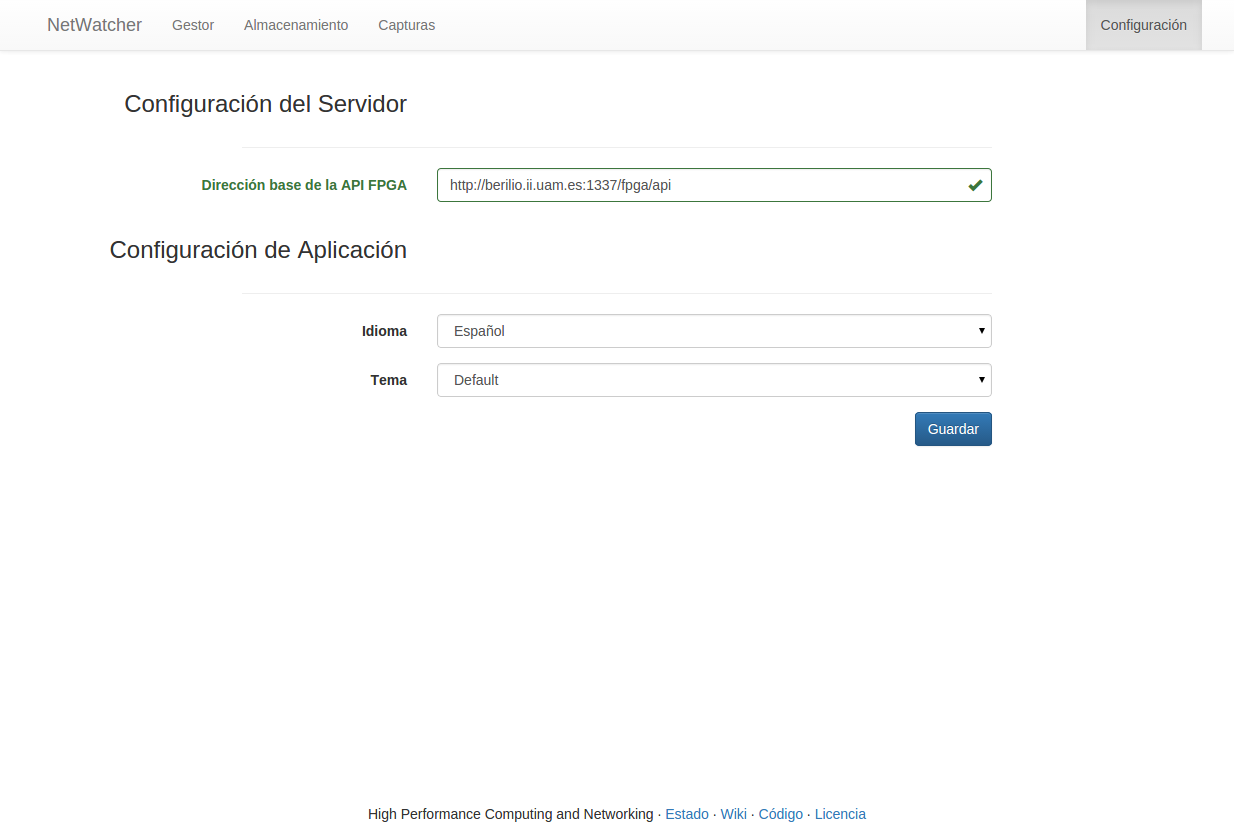
\includegraphics[width=0.9\textwidth,clip=true]{graphics/capturas/configuracion_tema_base}
  \caption{Página de configuración de la interfaz web.}
  \label{fig:captura:configuracion}
\end{figure}


\section{Uso de la aplicación\label{extra:manual:uso}}
Una vez instalados y configurados tanto el \gls{servicioweb} \gls{FPGA} como la interfaz web, ya se puede utilizar la interfaz.
Esta interfaz se puede usar desde cualquier navegador, y tanto en ordenador como en móvil.
Todas las pantallas tienen las mismas barras de navegación.

Desde la barra de navegación superior se puede acceder a las siguientes pantallas:
\begin{itemize}
  \item \textbf{Gestor}: administración de la \gls{FPGA}.
  \item \textbf{Almacenamiento}: estadísticas de almacenamiento y del \gls{RAID}, si está activo.
  \item \textbf{Capturas}: gestión de las \glspl{traza} almacenadas.
  \item \textbf{Configuración}: explicada en la sección~\ref{extra:manual:configweb}.
\end{itemize}

La barra de navegación inferior contiene los siguientes elementos:
\begin{itemize}
  \item \textbf{Estado}: enlace a la pantalla con estado actual del sistema.
  \item \textbf{Wiki}: enlace a la documentación del proyecto.
  \item \textbf{Código}: enlace al repositorio de código del proyecto.
  \item \textbf{Licencia}: despliega la licencia del proyecto.
\end{itemize}

Adicionalmente, se puede acceder a la documentación interna autogenerada del proyecto (en inglés) mediante las siguientes rutas relativas a la dirección base de la interfaz web:
\begin{itemize}
  \item \textbf{Documentación del \gls{servicioweb} \gls{FPGA}}: \texttt{/docs-back-end/}.
  \item \textbf{Documentación de la interfaz web}: \texttt{/docs-front-end/}.
\end{itemize}

En las siguientes subsecciones se explica cómo utilizar las principales pantallas interactivas de la interfaz web.


\subsection{Gestor\label{extra:manual:gestor}}

En esta pantalla se controla el estado de la \gls{FPGA}.
El contenido de esta pantalla, y por tanto las acciones disponibles, cambian según el estado actual de la \gls{FPGA}.

Si la \gls{FPGA} no ha sido inicializada, la pantalla de gestión permitirá seleccionar un modo en el que inicializarla:
\begin{itemize}
  \item \textbf{Reproductor}: permite reproducir \glspl{traza} en formato \gls{simple}.
  \item \textbf{Capturador}: permite capturar tráfico web, almacenándolo en una \gls{traza} en formato \gls{simple}.
\end{itemize}

\begin{figure}[!htp]
  \centering
  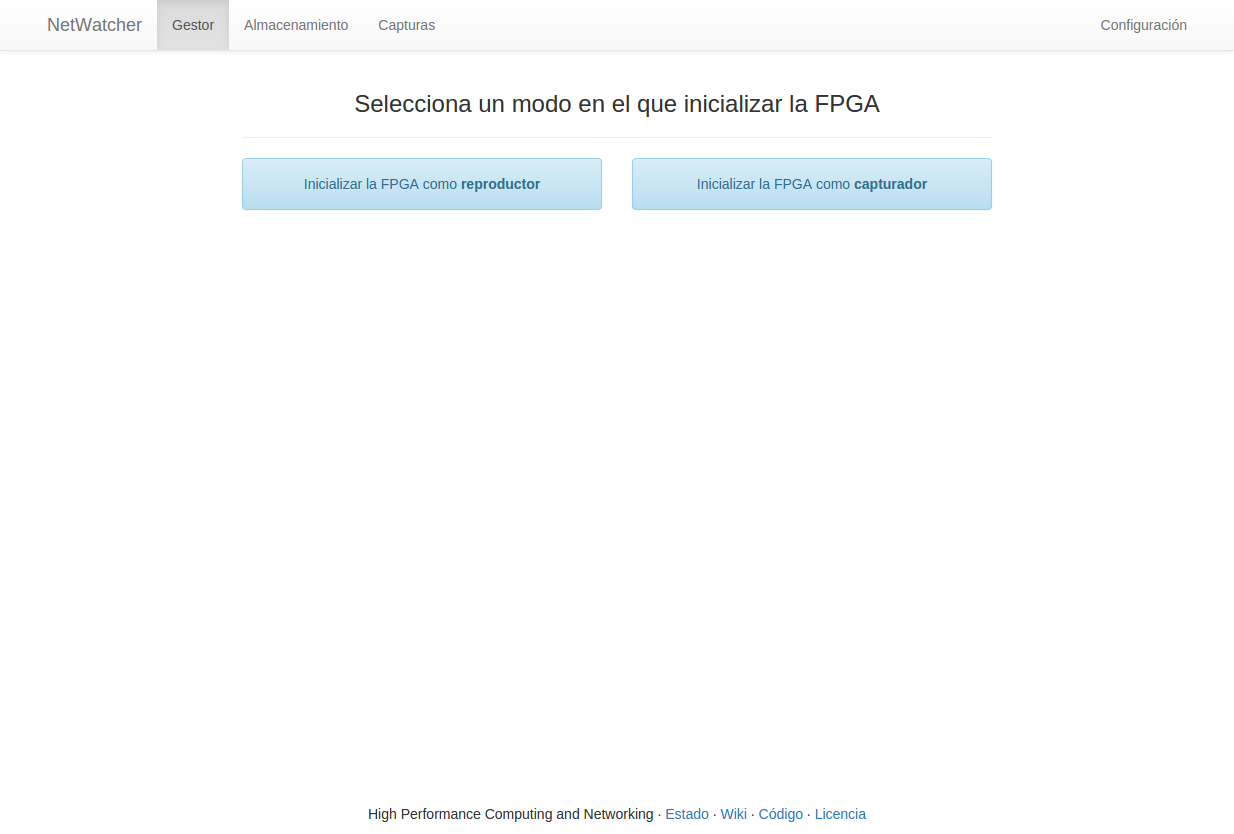
\includegraphics[width=0.9\textwidth,clip=true]{graphics/capturas/gestor_seleccion}
  \caption{Página de gestión - selección de modo.}
  \label{fig:captura:gestionseleccion}
\end{figure}

Para elegir un modo basta con pulsar uno de los dos botones de la interfaz (ver Figura~\ref{fig:captura:gestionseleccion}).
Esta elección de modo no es definitiva, ya que se puede cambiar de modo en cualquier momento siempre que la \gls{FPGA} no esté capturando o reproduciendo tráfico.

\begin{figure}[!htp]
  \centering
  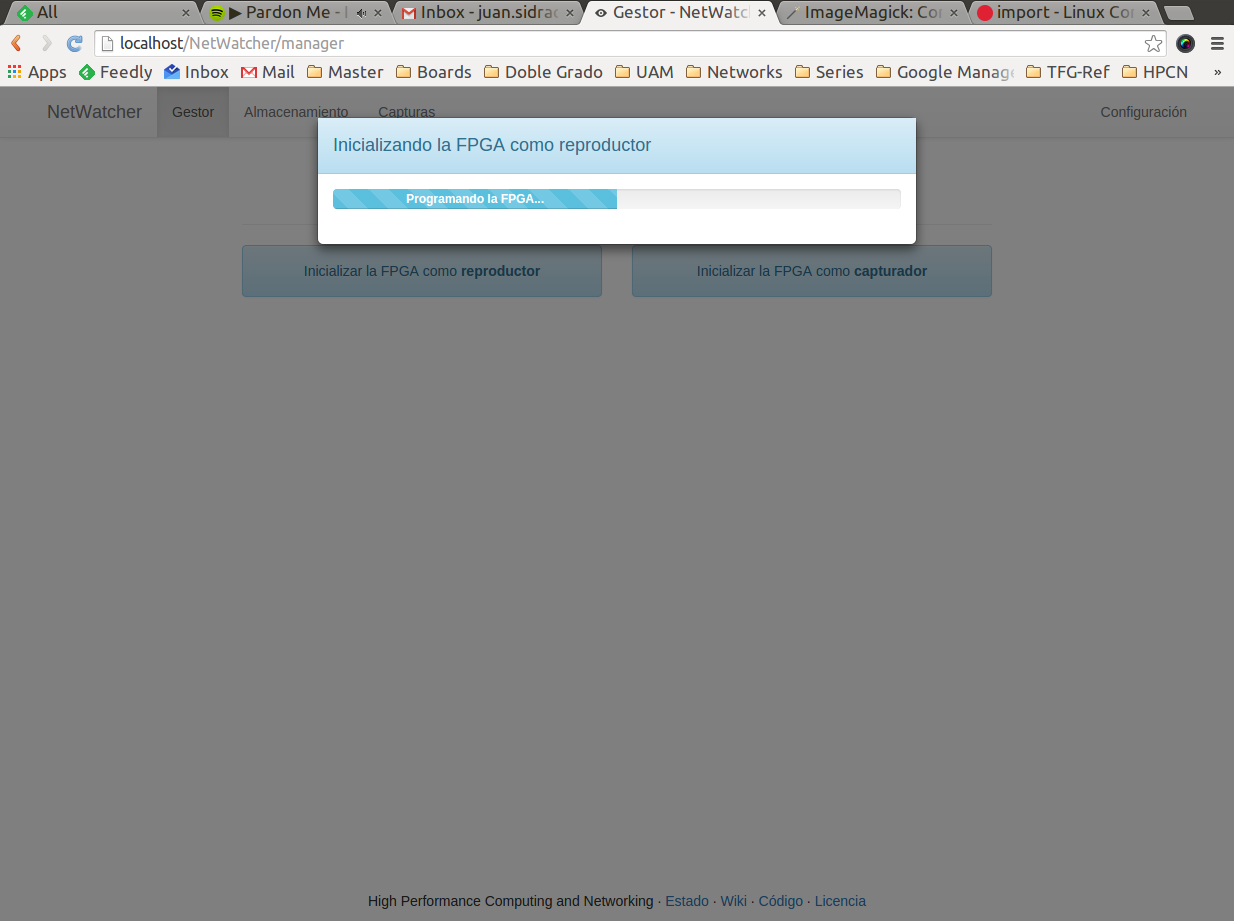
\includegraphics[width=0.9\textwidth,clip=true]{graphics/capturas/gestor_seleccion_progreso}
  \caption{Página de gestión - selección de modo en progreso.}
  \label{fig:captura:gestionprogreso}
\end{figure}

Una vez seleccionado un modo, un cuadro de diálogo muestra el progreso de la inicialización: programando la \gls{FPGA}, reiniciando el servidor y montando la \gls{FPGA} (ver Figura~\ref{fig:captura:gestionprogreso}).

\begin{figure}[!htp]
  \centering
  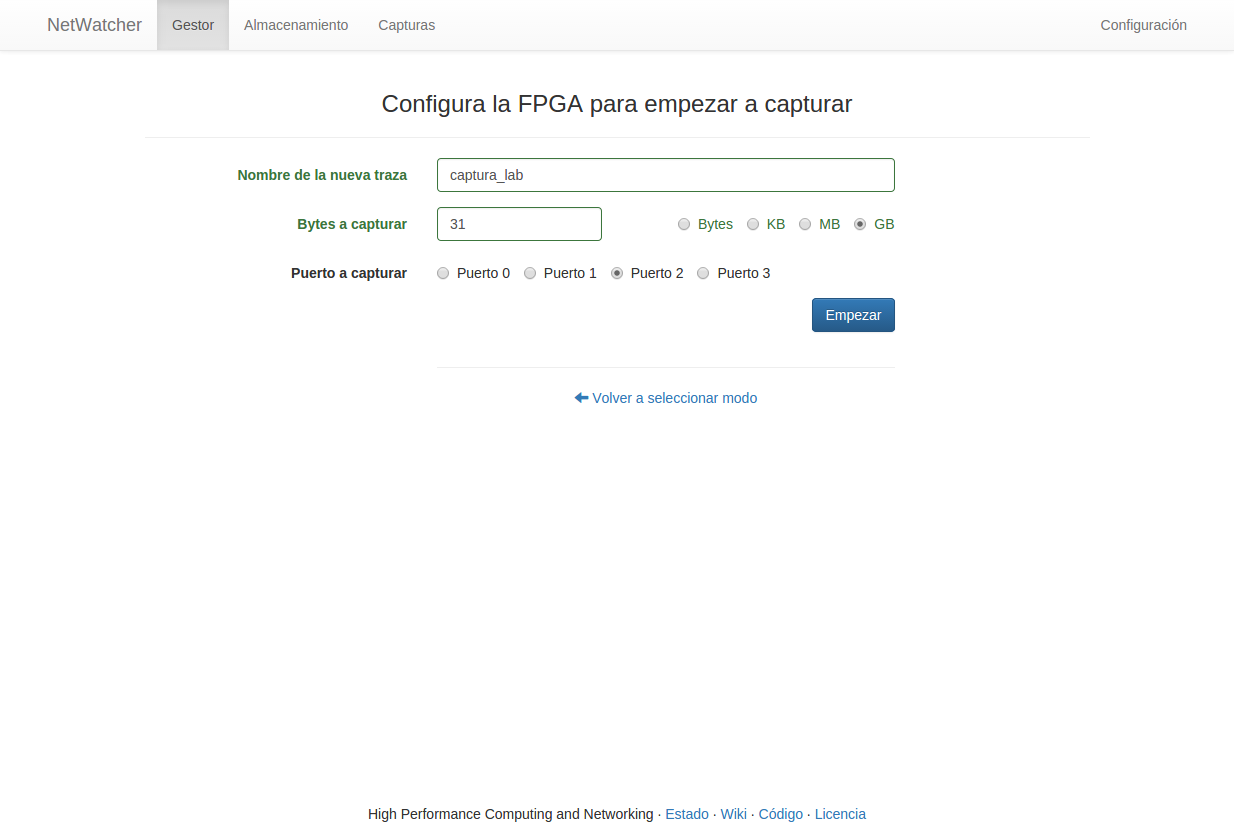
\includegraphics[width=0.9\textwidth,clip=true]{graphics/capturas/gestor_capturar}
  \caption{Página de gestión - capturar tráfico.}
  \label{fig:captura:gestioncapturar}
\end{figure}

Si la \gls{FPGA} ha sido inicializada en modo capturador, la pantalla de gestión mostrará un formulario en el que se configurarán los parámetros de una captura (ver Figura~\ref{fig:captura:gestioncapturar}).
Este formulario contiene los siguientes campos, todos ellos obligatorios:
\begin{itemize}
  \item \textbf{Nombre de la nueva \gls{traza}}: nombre que tendrá la \gls{traza} en la que se almacenará el tráfico capturado, en formato \gls{simple}.
  \item \textbf{Bytes a capturar}: número total de bytes que se capturarán, y su unidad (Bytes, KB, MB, GB).
  \item \textbf{Puerto a capturar}: puerto del que se capturará el tráfico entrante (0, 1, 2, 3).
\end{itemize}

Los dos primeros campos se iluminarán en verde cuando sean introducidos correctamente y en rojo cuando sean incorrectos.
Cuando todos los campos sean válidos se activará el botón de \textit{Empezar}, y si se pulsa la \gls{FPGA} comenzará a capturar tráfico con los parámetros indicados.

También es posible, en vez de capturar tráfico, volver a seleccionar modo pulsando el correspondiente enlace debajo del formulario.

\begin{figure}[!htp]
  \centering
  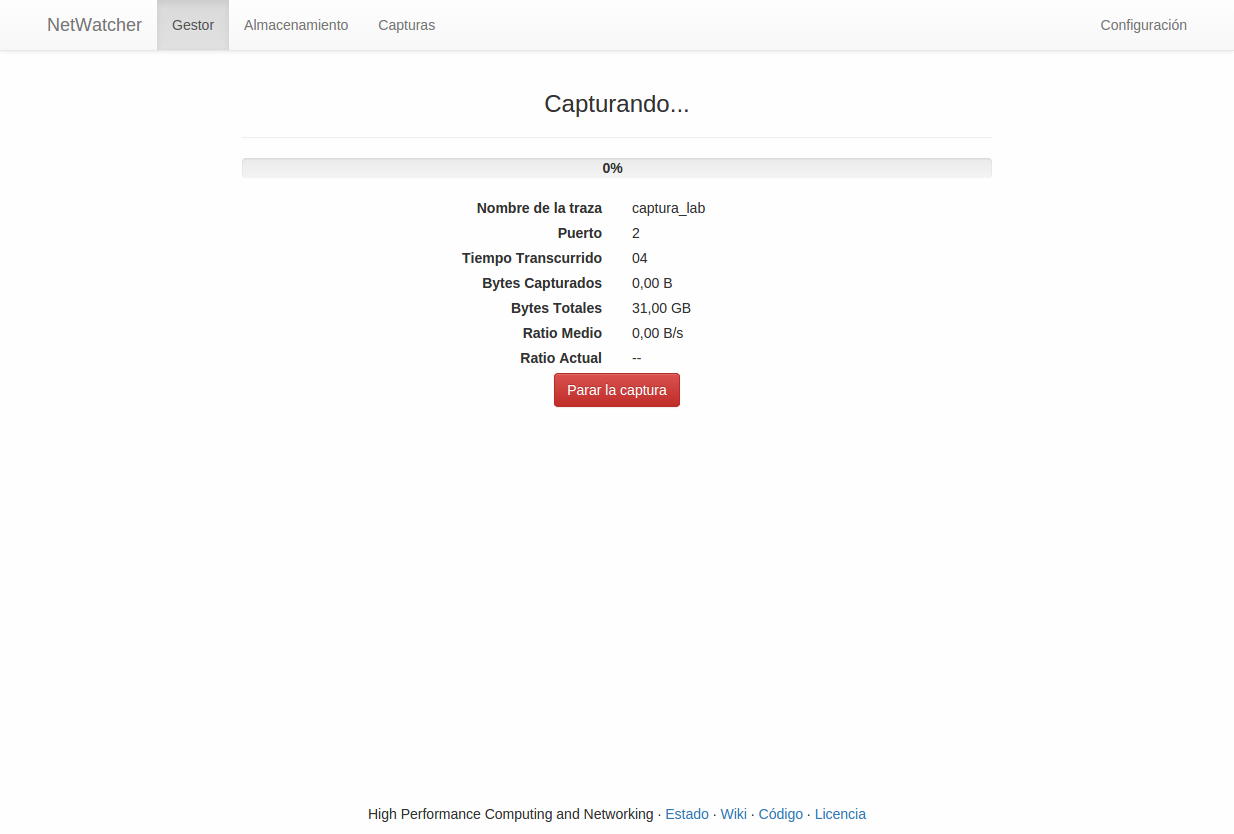
\includegraphics[width=0.9\textwidth,clip=true]{graphics/capturas/gestor_capturando}
  \caption{Página de gestión - capturando tráfico.}
  \label{fig:captura:gestioncapturando}
\end{figure}

Si la \gls{FPGA} está capturando tráfico, la pantalla de gestión mostrará el progreso de la captura en curso (ver Figura~\ref{fig:captura:gestioncapturando}).
Se podrán visualizar las siguientes estadísticas de la captura en curso:
\begin{itemize}
  \item \textbf{Nombre de la traza}: nombre de la \gls{traza} en la que se está almacenando el tráfico capturado, en formato \gls{simple}.
  \item \textbf{Puerto}: puerto del que se está capturando el tráfico entrante.
  \item \textbf{Tiempo transcurrido}: contador del tiempo que ha transcurrido desde que se inició la captura.
  \item \textbf{Bytes Capturados}: número de bytes que se han capturado ya.
  \item \textbf{Bytes Totales}: número total de bytes a capturar.
  \item \textbf{Ratio Medio}: velocidad media a la que se está capturando (estimación a partir de los bytes capturados y el tiempo transcurrido).
  \item \textbf{Ratio Actual}: velocidad a la que se ha capturado el tráfico desde la última actualización.
\end{itemize}

Se puede detener la captura en curso pulsando el botón de \textit{Parar la captura}, y se borrará lo almacenado hasta el momento en la \gls{traza}.

\begin{figure}[!htp]
  \centering
  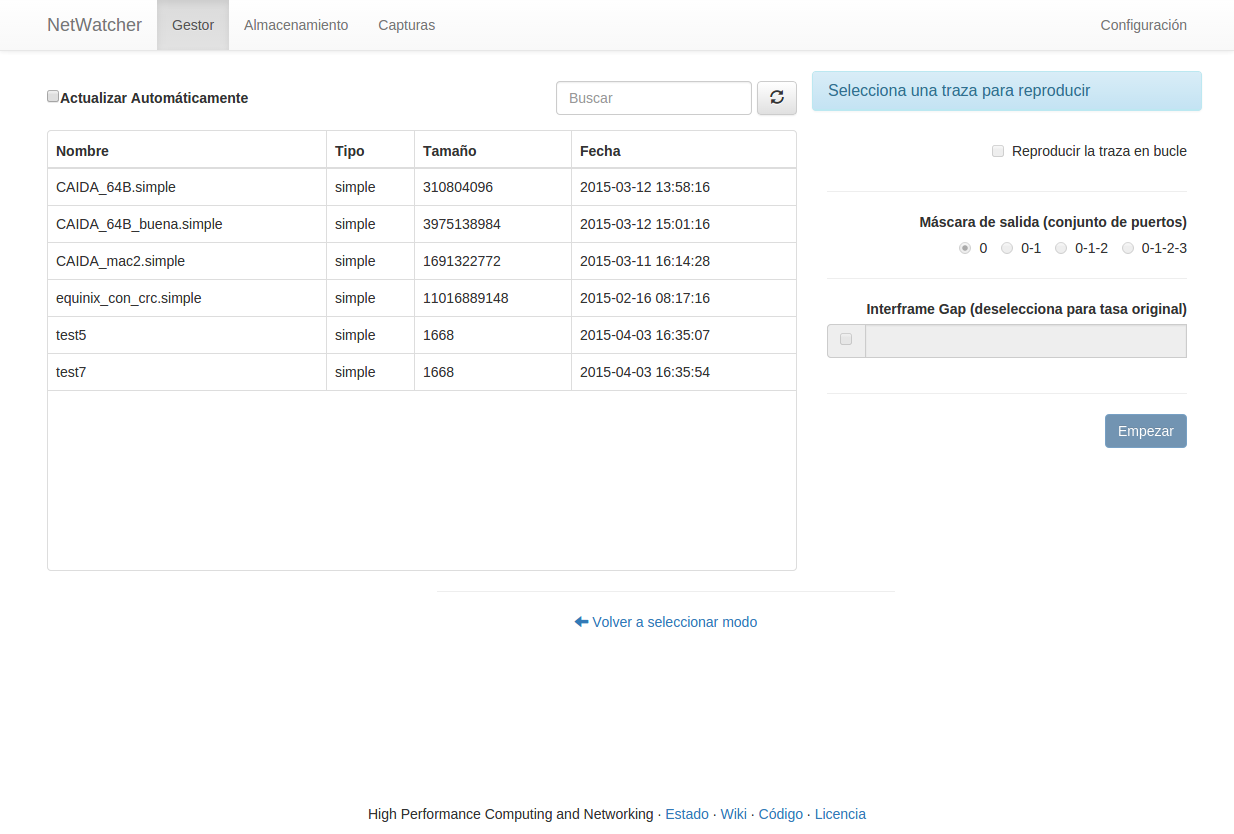
\includegraphics[width=0.9\textwidth,clip=true]{graphics/capturas/gestor_reproducir}
  \caption{Página de gestión - reproducir \gls{traza}.}
  \label{fig:captura:gestionreproducir}
\end{figure}

Si la \gls{FPGA} ha sido inicializada en modo reproductor, la pantalla de gestión mostrará una tabla y un formulario (ver Figura~\ref{fig:captura:gestionreproducir}).
La tabla contiene una fila por cada \gls{traza} disponible, con su nombre, tipo (\gls{simple}), tamaño y fecha.
Además, una barra superior asociada a esta tabla permite controlar el contenido de la misma mediante las siguientes acciones (de izquierda a derecha): activar la actualización automática de las \glspl{traza} disponibles, buscar una \gls{traza} por su nombre y actualizar manualmente las \glspl{traza} disponibles.
Pulsando sobre una fila de la tabla se seleccionará la \gls{traza} correspondiente para su reproducción.
Por otra parte, el formulario contiene los siguientes campos:
\begin{itemize}
  \item \textbf{Reproducir la \gls{traza} en bucle}: si se habilita, la \gls{traza} se reproducirá en un bucle infinito.
  \item \textbf{Máscara de salida}: conjunto de puertos a los que se reproducirá la \gls{traza} (0, 0-1, 0-1-2, 0-1-2-3).
  \item \textbf{Interframe Gap}: pausa temporal entre paquetes (si se deshabilita, tasa original con la que se capturó la \gls{traza}).
\end{itemize}

Cuando se haya seleccionado una traza de la tabla y todos los campos del formulario sean válidos se activará el botón de \textit{Empezar}, y si se pulsa la \gls{FPGA} comenzará a reproducir la \gls{traza} seleccionada con los parámetros indicados.

También es posible, en vez de reproducir tráfico, volver a seleccionar modo pulsando el correspondiente enlace debajo del formulario.

\begin{figure}[!htp]
  \centering
  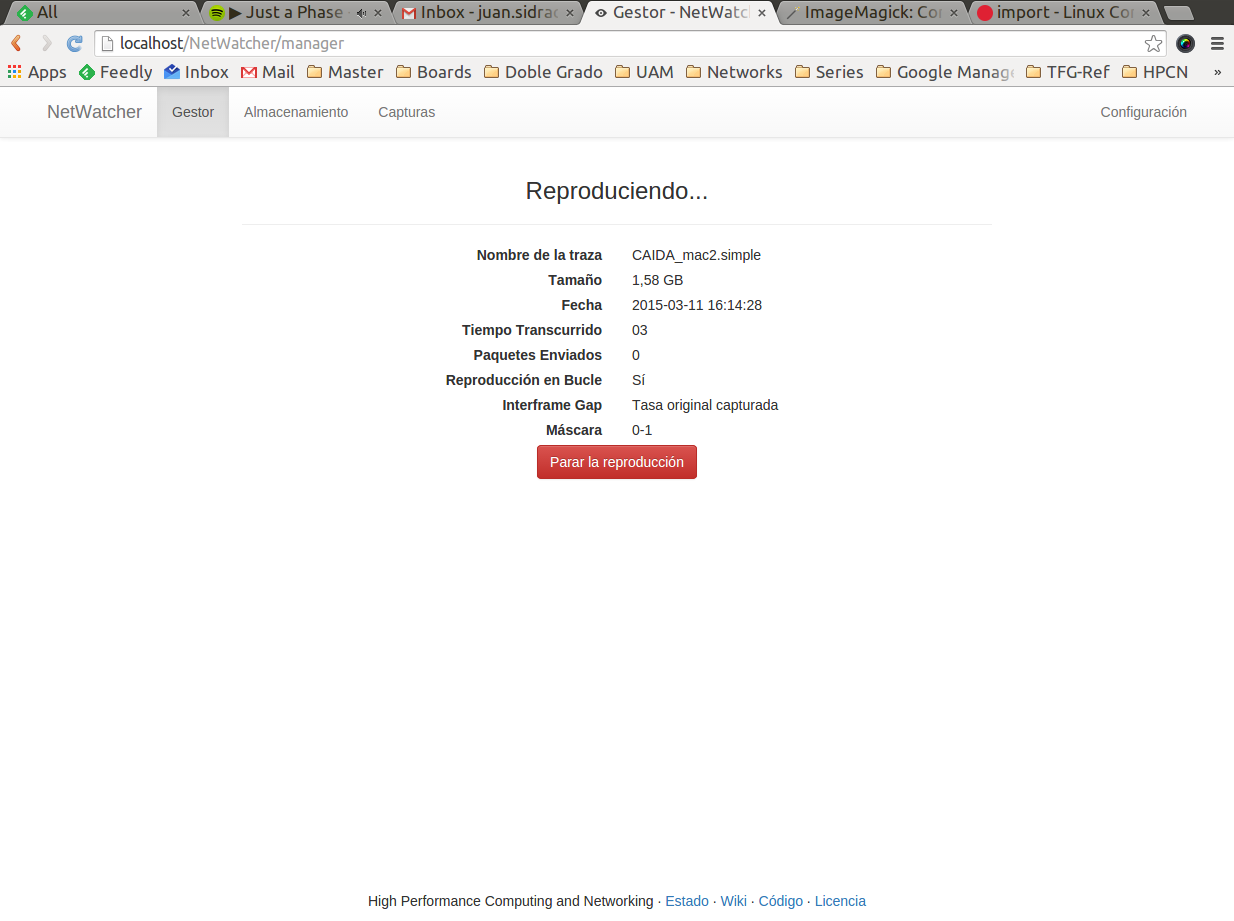
\includegraphics[width=0.9\textwidth,clip=true]{graphics/capturas/gestor_reproduccion}
  \caption{Página de gestión - reproduciendo \gls{traza}.}
  \label{fig:captura:gestionreproduciendo}
\end{figure}

Si la \gls{FPGA} está reproduciendo una \gls{traza}, la pantalla de gestión mostrará el progreso de la reproducción en curso (ver Figura~\ref{fig:captura:gestionreproduciendo}).
Se podrán visualizar las siguientes estadísticas de la reproducción en curso:
\begin{itemize}
  \item \textbf{Nombre de la \gls{traza}}: nombre de la \gls{traza} que se está reproduciendo.
  \item \textbf{Tamaño}: número de bytes que ocupa la \gls{traza} que se está reproduciendo.
  \item \textbf{Fecha}: fecha en que se creó la \gls{traza} que se está reproduciendo.
  \item \textbf{Tiempo Transcurrido}: contador del tiempo que ha transcurrido desde que se inició la captura.
  \item \textbf{Paquetes Enviados}: número de paquetes que se han enviado en la reproducción actual.
  \item \textbf{Reproducción en Bucle}: indica si se está reproduciendo la \gls{traza} en un bucle infinito o no.
  \item \textbf{Interframe Gap}: valor del \gls{IFG} en la reproducción actual.
  \item \textbf{Máscara}: conjunto de puertos en los que se está reproduciendo la \gls{traza} seleccionada (0, 0-1, 0-1-2, 0-1-2-3).
\end{itemize}

Se puede detener la reproducción en curso pulsando el botón \textit{Parar la reproducción}.


\subsection{Almacenamiento\label{extra:manual:almacenamiento}}

En esta pantalla se pueden visualizar distintas estadísticas de almacenamiento del sistema.
Está compuesta por dos paneles:

\begin{itemize}
\item \textbf{Estadísticas de espacio (Figura~\ref{fig:captura:espacio})}: este panel muestra estadísticas del espacio total, ocupado y disponible, resumido además en un gráfico circular (en rojo la proporción de disco ocupado y en turquesa la proporción de disco disponible).
\begin{figure}[!htp]
  \centering
  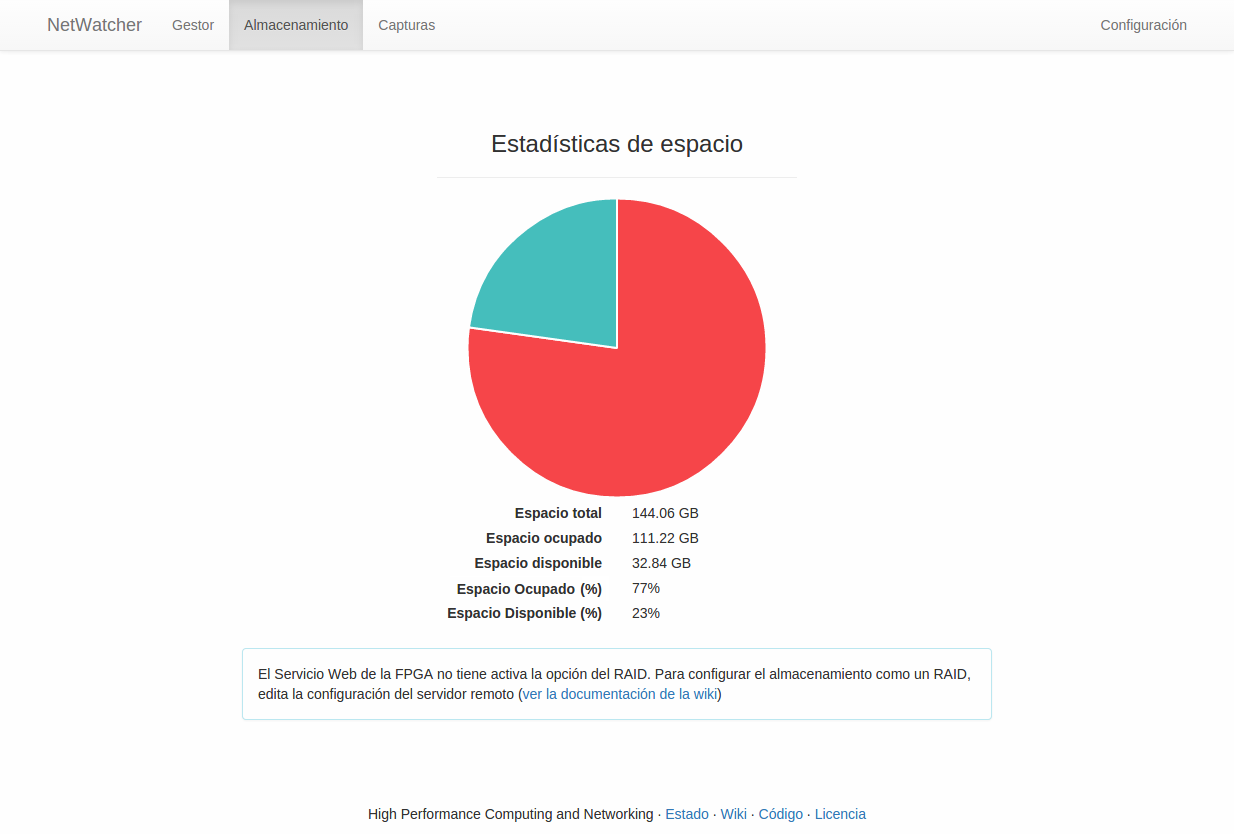
\includegraphics[width=0.9\textwidth,clip=true]{graphics/capturas/almacenamiento_espacio}
  \caption{Página de almacenamiento, con \gls{RAID} no activo.}
  \label{fig:captura:espacio}
\end{figure}

\item \textbf{Estadísticas del \gls{RAID} (Figura~\ref{fig:captura:raid})}: solo se mostrarán estas estadísticas si el sistema de almacenamiento está configurado como un \gls{RAID} (ver sección~\ref{extra:manual:configfpga}).
En este panel, un gráfico de barras muestra la velocidad de escritura de cada disco del \gls{RAID}.
Debajo de este gráfico se indica la velocidad global de escritura del \gls{RAID}.
El color de esta cifra depende de la velocidad de escritura: verde (velocidad superior a la recomendada), amarillo (velocidad suficiente) o rojo (velocidad por debajo del mínimo aceptable).
Si la velocidad es insuficiente se mostrará un cuadro de diálogo adicional para formatear y recrear el \gls{RAID} pulsando el botón \textit{Formatear el \gls{RAID}} (cuidado: formatear el \gls{RAID} borrará todos los datos del mismo).
Este diálogo se puede ocultar pulsando el botón \textit{Descartar}.
\begin{figure}[!htp]
  \centering
  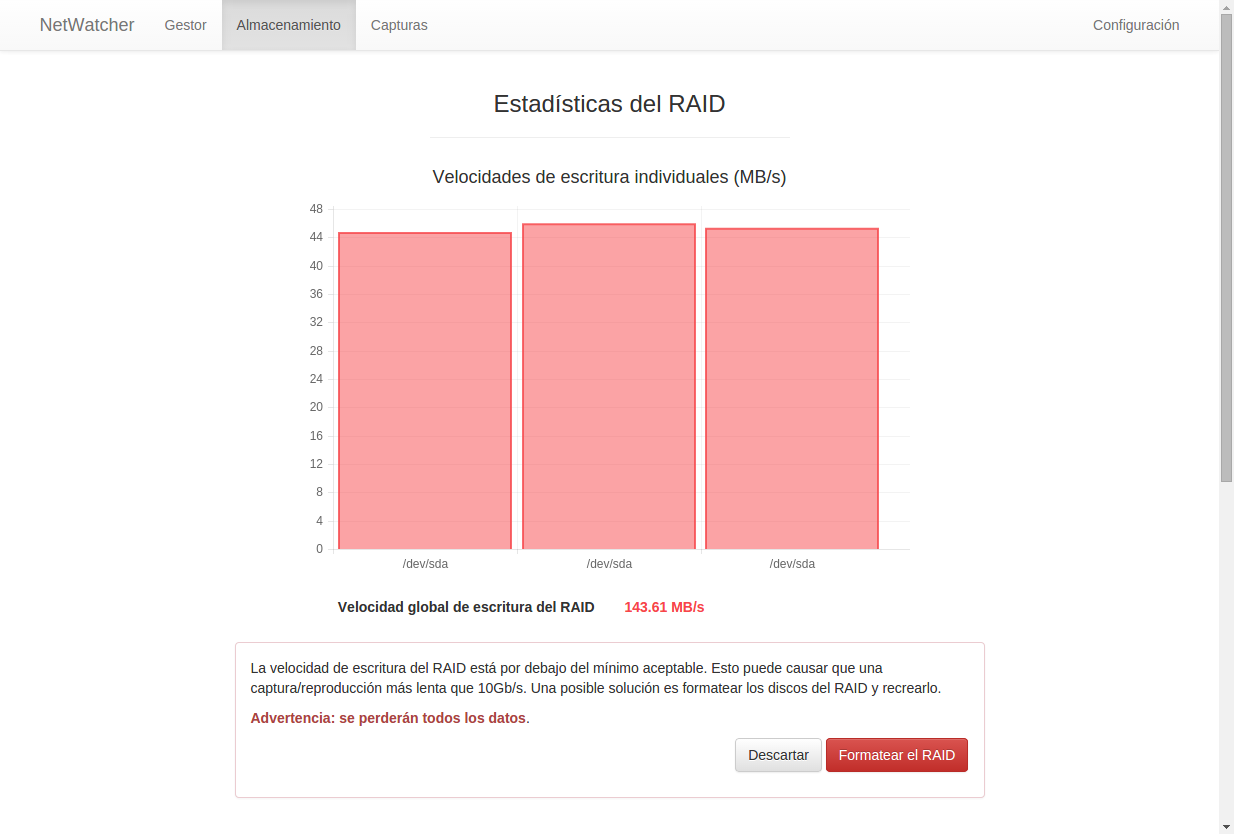
\includegraphics[width=0.9\textwidth,clip=true]{graphics/capturas/almacenamiento_raid}
  \caption{Página de almacenamiento, con \gls{RAID} activo.}
  \label{fig:captura:raid}
\end{figure}
\end{itemize}


\subsection{Capturas\label{extra:manual:capturas}}

\begin{figure}[!htp]
  \centering
  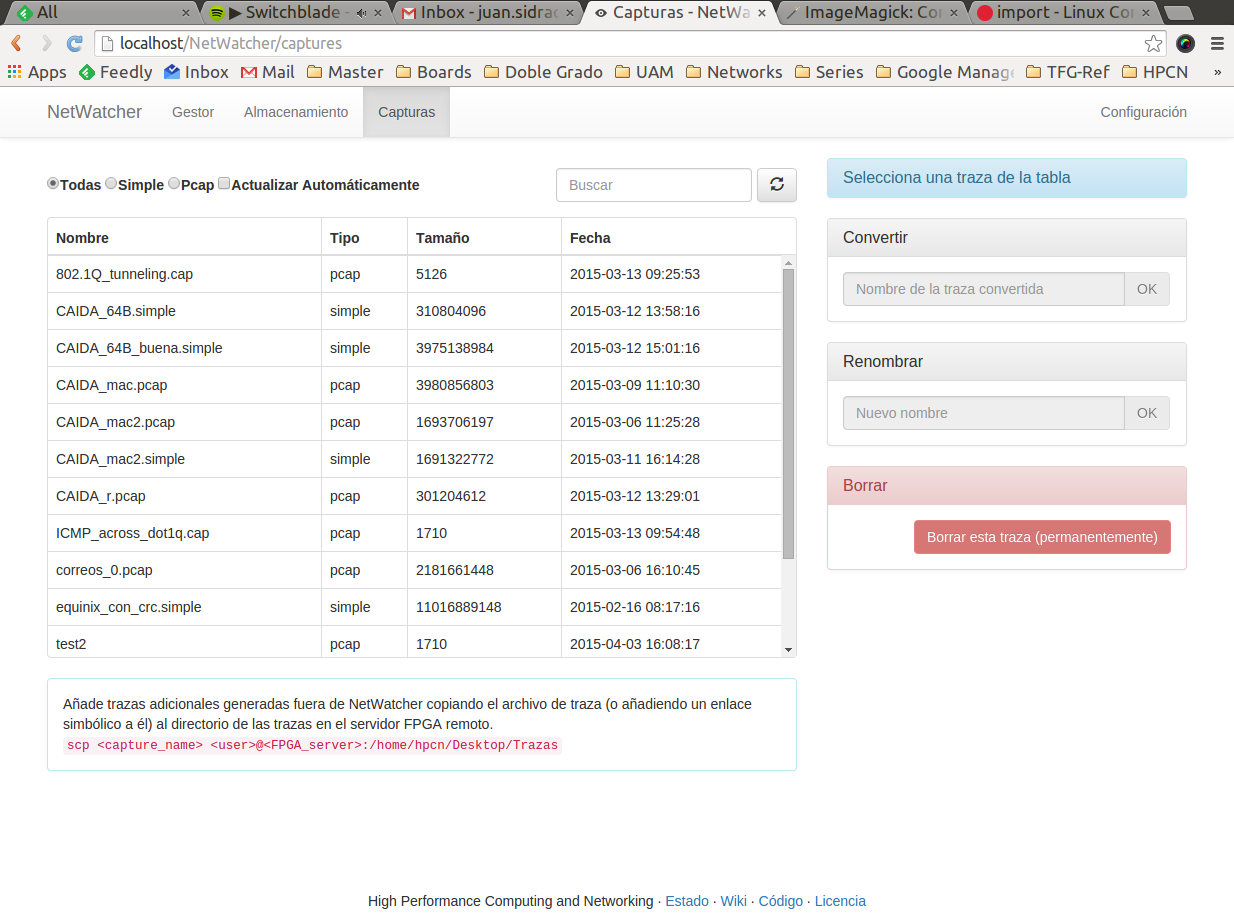
\includegraphics[width=0.9\textwidth,clip=true]{graphics/capturas/capturas}
  \caption{Página de capturas.}
  \label{fig:captura:capturas}
\end{figure}

En esta pantalla se pueden gestionar las \glspl{traza} almacenadas (ver Figura~\ref{fig:captura:capturas}), mediante una tabla y un panel de acciones.
La tabla contiene una fila por cada \gls{traza} disponible, con su nombre, tipo, tamaño y fecha.
Además, una barra superior asociada a esta tabla permite controlar el contenido de la misma mediante las siguientes acciones (de izquierda a derecha): filtrar las \glspl{traza} que se muestran según su tipo, activar la actualización automática de las \glspl{traza} disponibles, buscar una \gls{traza} por su nombre y actualizar manualmente las \glspl{traza} disponibles.
Pulsando sobre una fila de la tabla se seleccionará la \gls{traza} correspondiente, activándose el panel de acciones.
Este panel permite, mediante cada uno de sus subpaneles, las siguientes operaciones:
\begin{itemize}
  \item \textbf{Convertir}: crea una nueva \gls{traza} a partir de la \gls{traza} seleccionada cambiando el tipo (si la original tiene formato \gls{simple} la convertida tendrá formato \gls{pcap}, y viceversa).
  \item \textbf{Renombrar}: cambia el nombre de la \gls{traza} seleccionada al nuevo nombre introducido.
  \item \textbf{Borrar}: borra del disco la \gls{traza} seleccionada.
\end{itemize}

Los dos primeros subpaneles permitirán realizar su acción (se activará el correspondiente botón de \textit{OK}) cuando el campo de texto asociado a cada operación sea introducido correctamente.


\subsection{Estado\label{extra:manual:estado}}

\begin{figure}[!htp]
  \centering
  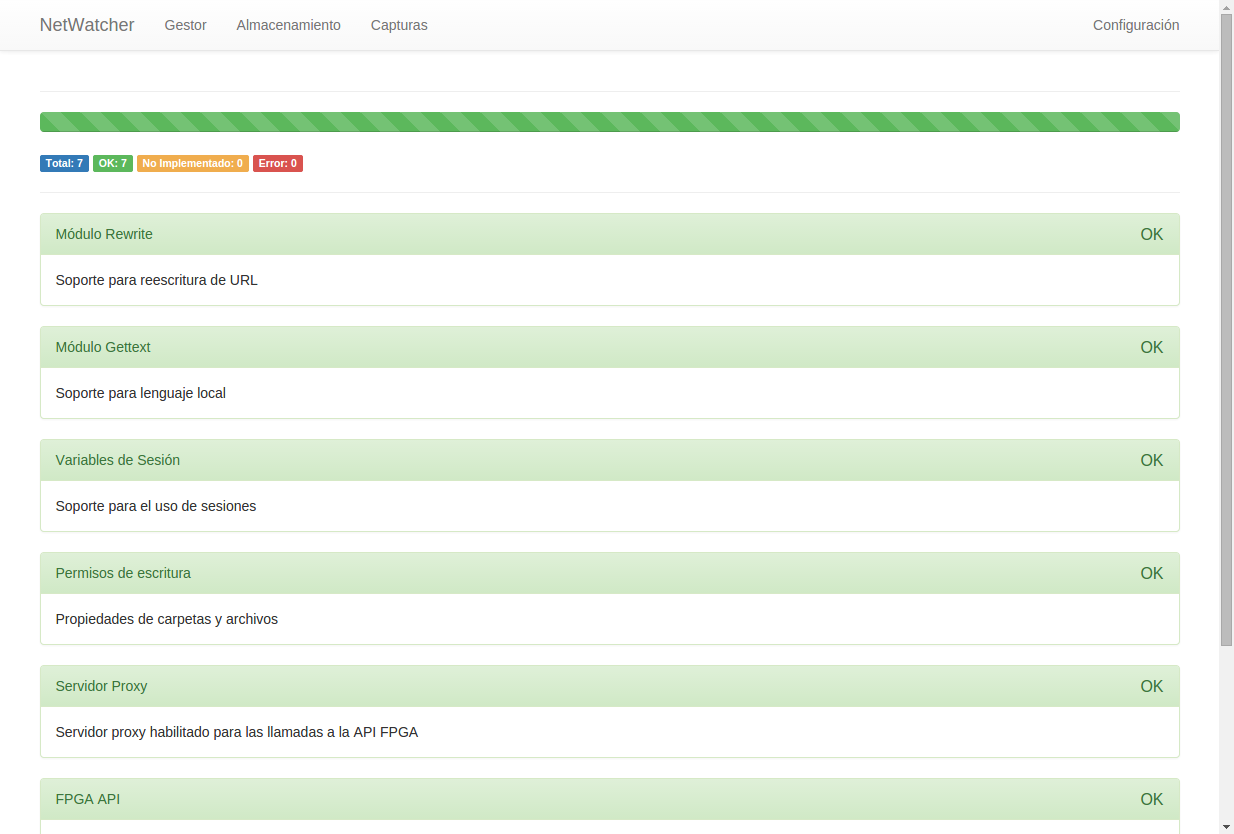
\includegraphics[width=0.9\textwidth,clip=true]{graphics/capturas/estado}
  \caption{Página de estado del sistema.}
  \label{fig:captura:estado}
\end{figure}

En esta pantalla se puede comprobar el estado de los distintos componentes que forman la aplicación (ver Figura~\ref{fig:captura:estado}).
Cada componente tiene un test asociado cuyo resultado se refleja en un panel.
Cada test puede tener tres resultados distintos: \textit{OK} (test pasado, en verde), \textit{No Implementado} (test no implementado, en amarillo) y \textit{Error} (test fallado, en rojo).
Los componentes sobre los que se comprueba su estado son los siguientes:
\begin{itemize}
  \item \textbf{Módulo Rewrite}: soporte para reescritura de \gls{URL}.
  \item \textbf{Módulo Gettext}: soporte para localización (traducción a distintos idiomas).
  \item \textbf{Variables de Sesión}: soporte para el uso de sesiones en \gls{PHP}.
  \item \textbf{Permisos de escritura}: permisos para escribir \textit{logs} y archivos de configuración.
  \item \textbf{Servidor Proxy}: servidor proxy habilitado para llamadas a la API \gls{FPGA}.
  \item \textbf{\gls{FPGA} API}: servidor de la \gls{FPGA} activo.
  \item \textbf{Relojes Sincronizados}: diferencia de relojes entre el cliente y el servidor \gls{FPGA} dentro del umbral permitido.
\end{itemize}

Adicionalmente, una barra de progreso encima de todo los paneles resume el estado global del sistema.


\section{Solución de problemas\label{extra:manual:solucion}}

Si tras seguir las instrucciones paso a paso algo impide el correcto funcionamiento de la aplicación, se puede consultar la página de solución de problemas (en inglés), disponible dentro del repositorio del proyecto en:

\href{https://github.com/JSidrach/NetWatcher/blob/master/docs/wiki/Troubleshooting.md}{github.com/JSidrach/NetWatcher/blob/master/docs/wiki/Troubleshooting.md}

\chapter{Framework desarrollado\label{extra:frameworkDesarrollado}}

En este apéndice se explican los distintos componentes del \gls{framework} desarrollado en el que se ha implementado la interfaz web.
Este \gls{framework} está implementado en \gls{PHP} sobre \textit{Apache httpd}~\cite{httpd}.
Sirve de base para la organización y desarrollo de la aplicación, proveyéndola de un gestor de rutas, un patrón de arquitectura para los módulos de la aplicación (modelo-vista-controlador), un \gls{proxy} simplificado para las llamadas al \gls{servicioweb} \gls{FPGA}, soporte para la internacionalización de la interfaz, gestión automática de dependencias, y registro de eventos (ver Figura~\ref{fig:framework}).

\begin{figure}[!htp]
  \centering
  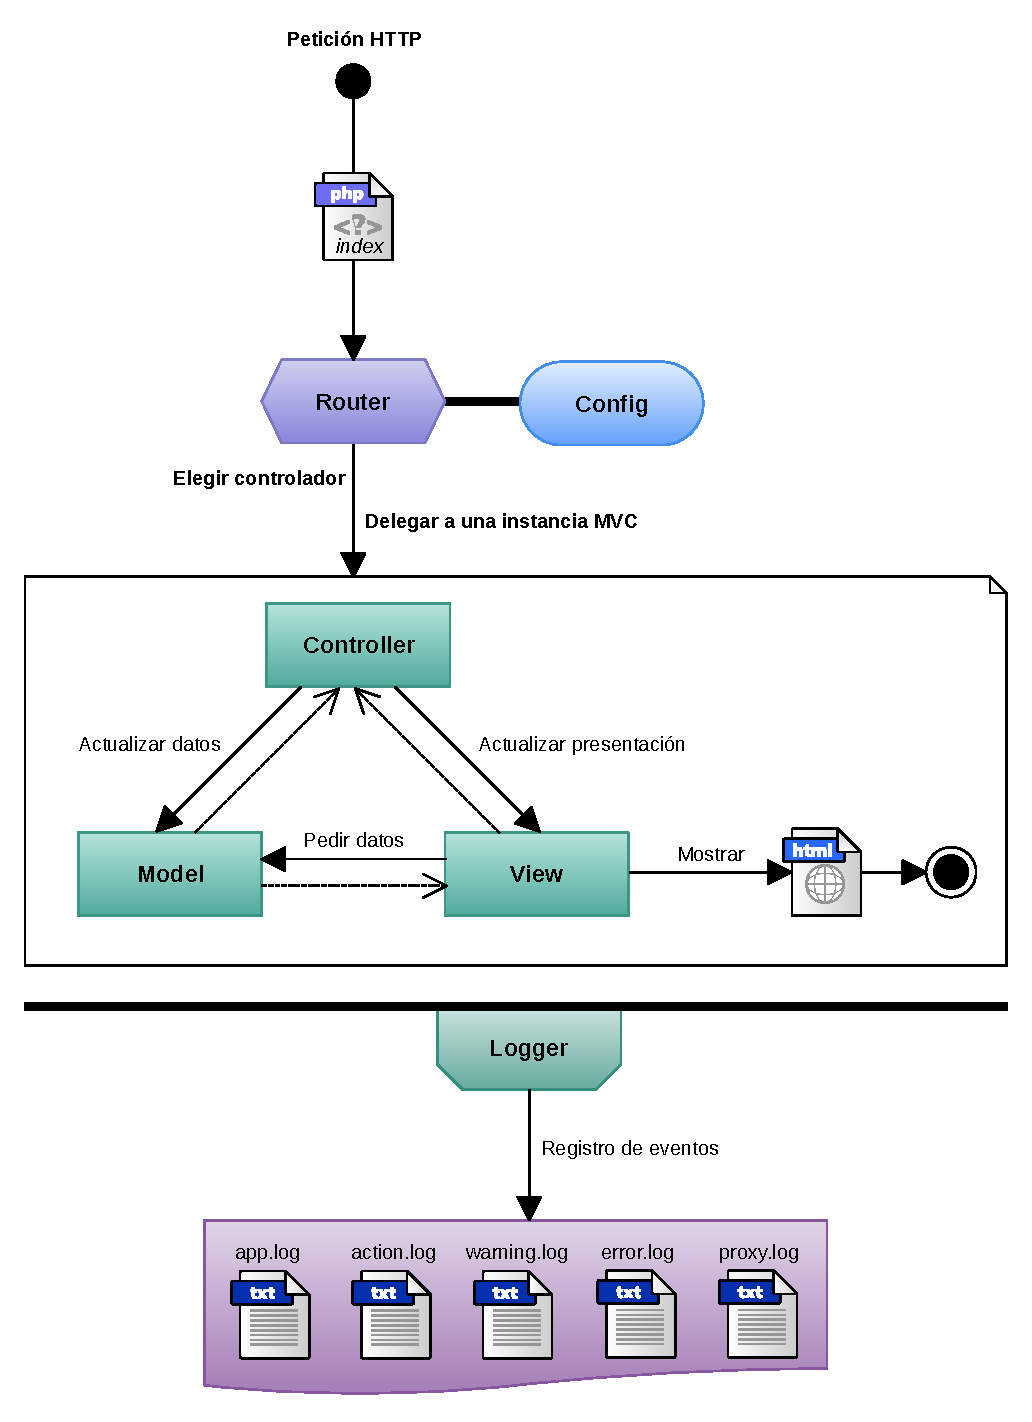
\includegraphics[width=\textwidth,clip=true]{graphics/framework}
  \caption{Arquitectura del \gls{framework} desarrollado.}
  \label{fig:framework}
\end{figure}


\section{Gestión de rutas\label{extra:mvc:router}}

El componente de gestión de rutas del \gls{framework} se encarga de interpretar las peticiones realizadas por el usuario y delegarlas al módulo apropiado.
Con este fin, todas las peticiones \gls{HTTP}, a excepción de las que van dirigidas al \textit{proxy} (ver sección~\ref{extra:mvc:proxy}), se redirigen utilizando \textit{mod\_rewrite}~\cite{modrewrite} al archivo \textit{index.php}.
Este archivo a su vez invoca el método estático \textit{Router->dispatch()}.

El método \textit{Router->dispatch()} divide la \gls{URL} solicitada siguiendo el siguiente formato:

\textit{URL\_BASE\_APLICACIÓN/módulo/método/parámetro1/parámetro2/...}

Una vez identificadas las partes de la \gls{URL}, se crea una instancia del módulo correspondiente y se llama al método indicado con los parámetros de la petición (si existiesen), delegándole el control de la solicitud (ver Figura~\ref{fig:router}).
Por otro lado, si la \gls{URL} acaba en la \gls{URL} base de la aplicación, se cargan el módulo y método por defecto; y si la \gls{URL} acaba en el módulo, se carga el método por defecto (ver sección~\ref{extra:mvc:config}).
En caso de que la \gls{URL} contenga un módulo o método no existente, se redirecciona la petición a la página de \textit{Error 404 - Página no encontrada}.

\begin{figure}[!htp]
  \centering
  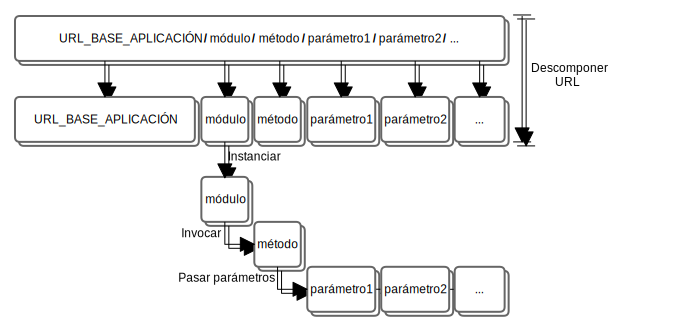
\includegraphics[width=\textwidth,clip=true]{graphics/router}
  \caption{Esquema de flujo del método \textit{Router->dispatch()}.}
  \label{fig:router}
\end{figure}


\section{Patrón de arquitectura para los módulos\label{extra:mvc:mvc}}

Las aplicaciones desarrolladas sobre el \gls{framework} se estructuran en módulos que siguen el patrón de arquitectura modelo-vista-controlador~\cite{mvcpattern}.
Este patrón separa la lógica de negocio de la interfaz de usuario, facilitando la evolución por separado de ambos aspectos e incrementando la reutilización y flexibilidad de los módulos de la aplicación.

Los componentes o capas de este patrón de arquitectura son:
\begin{itemize}
  \item \textbf{Modelo}: contiene el estado, los datos y la lógica interna de negocio.
  \item \textbf{Vista}: construye la representación del modelo.
  \item \textbf{Controlador}: gestiona las peticiones del usuario.
\end{itemize}

Cuando un usuario realiza una acción en la interfaz web, el controlador gestiona la solicitud notificando la acción al modelo, que se actualiza en consecuencia.
Posteriormente, el controlador ordena a la vista mostrar al usuario el nuevo estado de la aplicación.
La vista consulta entonces el nuevo modelo y lo representa, en el caso de este \gls{framework} en forma de página web.

Las clases abstractas \textit{Model}, \textit{View} y \textit{Controller} incluidas en el \gls{framework} proporcionan una implementación base de este patrón.
Cada módulo de la aplicación debe heredar cada una de las tres clases e implementar en ellas su funcionalidad propia.


\section{Redireccionamiento de peticiones AJAX\label{extra:mvc:proxy}}

Por motivos de rendimiento (no sobrecargar el servidor del \gls{servicioweb} \gls{FPGA} incluyéndole también la interfaz) y disponibilidad (la interfaz web debe ser accesible aunque el \gls{servicioweb} \gls{FPGA} no esté operativo), el \gls{servicioweb} \gls{FPGA} y la interfaz web no están alojados en el mismo servidor.
Esto plantea un problema ya que se necesitan realizar peticiones \gls{AJAX} desde el cliente al \gls{servicioweb} \gls{FPGA}, y los navegadores web no permiten por motivos de seguridad que un cliente se comunique con un dominio distinto a la web original solicitada~\cite{sameorigin}.

Para resolver esto, el \gls{framework} contiene un servidor \gls{proxy} simplificado.
Este \gls{proxy} no es genérico, ya que siempre redirecciona a la dirección IP del \gls{servicioweb} \gls{FPGA}.
Así, cuando la interfaz web quiera realizar una petición \gls{AJAX} al \gls{servicioweb} \gls{FPGA}, hará la petición al servidor \gls{proxy}, éste redirigirá la petición al \gls{servicioweb} \gls{FPGA}, obtendrá la respuesta y la reenviará de vuelta al cliente (ver Figura~\ref{fig:proxy}).

\begin{figure}[!htp]
  \centering
  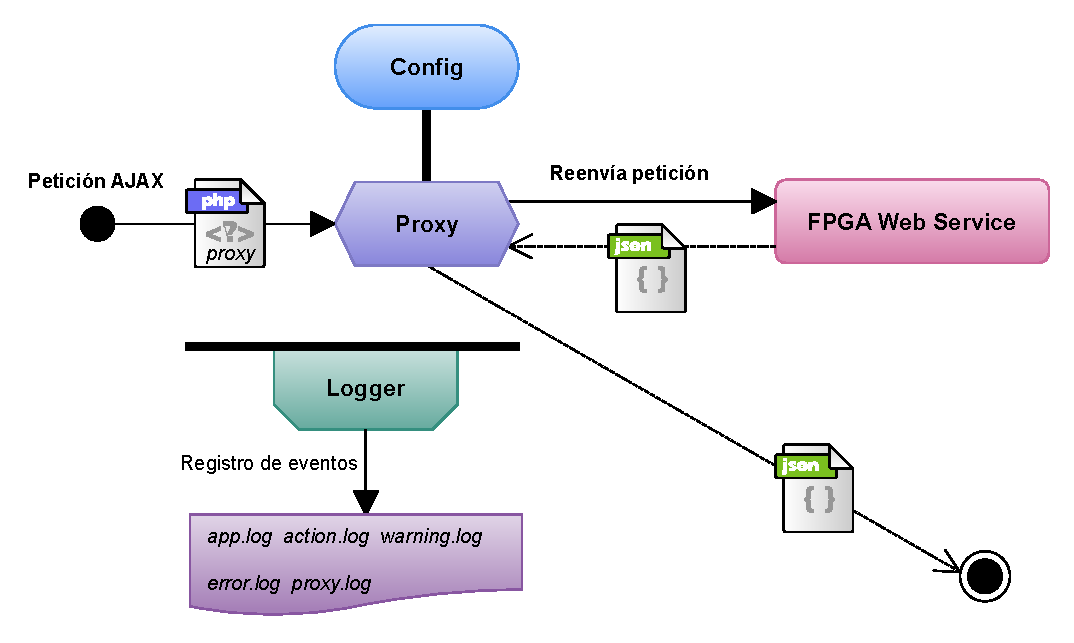
\includegraphics[width=0.6\textwidth,clip=true]{graphics/proxy}
  \caption{Arquitectura del proxy desarrollado.}
  \label{fig:proxy}
\end{figure}

\section{Internacionalización de la interfaz\label{extra:mvc:i18n}}

El \gls{framework} desarrollado facilita la traducción de la aplicación a distintos idiomas mediante la librería \textit{gettext}~\cite{gettext} para \gls{PHP}.
Esta librería proporciona funciones (``\textit{\_}'' y ``\textit{gettext}'') que reciben cadenas de texto y devuelven su equivalente en el idioma de la aplicación seleccionado, consultando un archivo previamente creado (catálogo) que contiene cadenas de texto originales y su traducción.

Es necesario un catálogo por cada idioma que se quiera añadir a la aplicación.
Los catálogos se almacenan en la carpeta del proyecto \texttt{./locale/}.
Para crear y gestionar los catálogos es recomendable utilizar la herramienta \textit{Poedit}~\cite{poedit}, que permite editarlos con una interfaz gráfica.
Para obtener las cadenas de texto que se necesitan traducir, se escanean todos archivos del proyecto en busca de las palabras clave, y se añaden las cadenas de texto al catálogo para su traducción por parte del desarrollador.

En el Código~\ref{code:ejemplogettext} se describe un ejemplo de cómo imprimir una cadena traducida a otro idioma mediante una llamada a la función ``\textit{\_}''.
Si el idioma base de los catálogos es el inglés y el idioma establecido en la aplicación es español, la función ``\textit{\_}'' busca la cadena en inglés (idioma base) \textit{`Example of string'} en el catálogo español y devuelve la cadena de texto \textit{`Ejemplo de cadena'}, que finalmente se imprime con \textit{echo}.

\begin{code}[label=code:ejemplogettext,language=php,caption=Ejemplo de traducción en \gls{PHP} con la librería \textit{gettext}]
/* Set the app language */
putenv('LANG=' . 'es_ES.utf8');
putenv('LANGUAGE=' . 'es_ES.utf8');
setlocale(LC_ALL, 'es_ES.utf8');
bindtextdomain('messages', 'locale');
bind_textdomain_codeset('messages', 'utf-8');
/* Print the example string */
echo _('Example of string');
\end{code}


\section{Gestión de dependencias\label{extra:mvc:dependencias}}

Como en la mayoría de proyectos, es conveniente poder utilizar librerías externas y no tener que invertir tiempo en resolver problemas que ya han sido solucionados por otros anteriormente, siempre que la solución encaje dentro de la propia aplicación.
Para manejar la descarga e instalación local de estas librerías externas se han elegido dos gestores de dependencias: \textit{Composer}~\cite{composer} para el \gls{back-end} y \textit{BowerPHP}~\cite{bowerphp} para el \gls{front-end}.
Estos gestores permiten además tener un control sobre la versión exacta necesaria de cada librería, evitando así incompatibilidades.

\subsection*{Composer\label{extra:mvc:composer}}

\textit{Composer} es un gestor de dependencias y requisitos \gls{back-end} para \gls{PHP}.
Las librerías externas \gls{back-end} que se necesitan para la aplicación se declaran, una vez localizadas en el repositorio de paquetes de \textit{Composer}~\cite{composerrepositorio}, en el archivo \texttt{composer.json} (ver Código~\ref{code:composerjson}).
\textit{Composer} posibilita también, siguiendo el estándar PSR-4~\cite{psr4}, incluir en una sola línea de código \gls{PHP} tanto las dependencias de librerías externas como módulos propios:

\texttt{require\_once ('vendor/autoload.php')};

Las dependencias se descargan e instalan de forma local al proyecto ejecutando el \gls{script} \texttt{./scripts/build.sh ----install}.

\begin{code}[label=code:composerjson,language=json,caption=Ejemplo de fichero \textit{composer.json}]
{
  "name": "NetWatcher",
  "type": "project",
  "license": "MIT",
  "authors": [
    {
      "name": "JSidrach",
      "email": "***REMOVED***",
      "role": "Developer"
    }
  ],
  "config": {
    "vendor-dir": "vendor/"
   },
  "require": {
    "php": ">=5.5.0",
    "beelab/bowerphp": "dev-master"
  },
  "autoload": {
    "psr-4": {
      "Core\\": "lib/"
    }
  }
}
\end{code}

\subsection*{BowerPHP\label{extra:mvc:bowerphp}}

\textit{BowerPHP} es una implementación en \gls{PHP} de \textit{Bower}~\cite{bower}, un gestor de dependencias \gls{front-end} para aplicaciones web.
Las librerías externas que se necesitan para la aplicación se declaran, una vez localizadas en el repositorio de paquetes de \textit{Bower}~\cite{bowerrepositorio}, en el archivo \texttt{bower.json} (ver Código~\ref{code:bowerjson}).
Las dependencias se descargan e instalan de forma local al proyecto ejecutando el \gls{script} \texttt{./scripts/build.sh ----install}.

\begin{code}[label=code:bowerjson,language=json,caption=Ejemplo de fichero \textit{bower.json}]
{
  "name": "NetWatcher",
  "authors": [
    "JSidrach <***REMOVED***>"
  ],
  "private": true,
  "dependencies": {
    "jquery": "2.*",
    "bootstrap": "3.*",
    "bootstrap-table": "1.*",
    "remarkable-bootstrap-notify": "3.*",
    "animate.css": "3.*",
    "chartjs": "1.*"
  }
}
\end{code}

\section{Configuración\label{extra:mvc:config}}

Para la configuración interna de la aplicación se utiliza la clase \textit{Config}, compuesta por métodos estáticos.
En esta clase se definen también las variables globales de la aplicación: nombres de carpetas y archivos, módulo a cargar por defecto, método a invocar por defecto, dirección IP del \gls{servicioweb} \gls{FPGA}, idiomas disponibles, idioma por defecto, temas visuales disponibles y tema visual por defecto.

Las variables que puede cambiar el usuario (idioma por defecto, tema visual por defecto y dirección IP del \gls{servicioweb} \gls{FPGA}) no se inicializan por definición en el código sino que se leen de distintos ficheros de la carpeta \texttt{./config/} en formato \gls{JSON}.

La configuración global de la aplicación se carga siempre al principio, mediante una llamada al método estático \textit{load} de la clase \textit{Config}.

\section{Registro de eventos\label{extra:mvc:logger}}

Registrar todos los eventos asociados a la aplicación es muy útil, ya que permite conocer cómo el usuario utiliza la aplicación y solucionar problemas internos.
Para ello, se utiliza la clase \textit{Logger}, que contiene métodos estáticos con los que registrar eventos manualmente dentro del código del proyecto.
Adicionalmente, utilizando las funciones estándar de \gls{PHP} \textit{set\_exception\_handler} y \textit{set\_error\_handler}, se redirigen los errores y excepciones a funciones que los registran (de la clase \textit{Logger} también).

Cada evento se guarda en un registro (línea de texto) precedido de la fecha y hora en que se produjo, así como la dirección IP del usuario.
Los registros se almacenan en diferentes ficheros dentro de la carpeta \texttt{./log/}:
\begin{itemize}
  \item \texttt{app.log}: registro general, contiene todos los eventos de la aplicación.
  \item \texttt{action.log}: contiene registros de los eventos relacionados con acciones del usuario.
  \item \texttt{proxy.log}: contiene registros de los eventos relacionados con las peticiones al módulo proxy.
  \item \texttt{warning.log}: contiene registros de los eventos relacionados con avisos y advertencias.
  \item \texttt{error.log}: contiene registros de los errores de la aplicación.
\end{itemize}


\section{Scripts adicionales\label{extra:mvc:scripts}}

Para automatizar tareas que se realizan con frecuencia en el desarrollo de la aplicación, este \gls{framework} contiene una carpeta (\texttt{./scripts/}) con \glspl{script} con este propósito, que pueden ser invocados desde la carpeta raíz del proyecto ejecutando el archivo \texttt{./scripts/build.sh} con distintos parámetros:
\begin{itemize}
  \item \texttt{----doc}: genera la documentación automática a partir del código del \gls{front-end} y del \gls{back-end}, en la carpeta \texttt{./docs/}.
  \item \texttt{----upgrade}: actualiza las librerías externas necesarias para la aplicación.
  \item \texttt{----install}: instala las dependencias externas (paquetes y librerías) necesarias para la aplicación.
  \item \texttt{----check}: realiza un análsis léxico y sintáctico sobre todo el código \gls{PHP} de la aplicación.
  \item \texttt{----permissions}: otorga los permisos mínimos necesarios de lectura/escritura/ejecución a los archivos y carpetas del proyecto.
  \item \texttt{----clear}: borra los archivos de \textit{logs}.
  \item \texttt{----backup}: comprime la carpeta del proyecto en un archivo en formato \textit{.zip}, y lo guarda con la fecha actual en la carpeta superior a modo de copia de seguridad.
\end{itemize}

\section{Conclusiones\label{extra:mvc:conclusiones}}

Se ha desarrollado un \gls{framework} que sirve de base para la interfaz web, proporcionando un conjunto mínimo de funcionalidad necesaria para el problema planteado.
Aunque desarrollarlo ha supuesto un coste temporal adicional para el proyecto, ha repercutido positivamente en fases posteriores de la implementación.

Conocer al detalle el \gls{framework} sobre el que se basa la aplicación y tener un control total sobre el mismo ha permitido agilizar el proceso de desarrollo.
Además, se ha adquirido experiencia en distintos conceptos útiles: orientación a objetos en \gls{PHP}, patrón de diseño modelo-vista-controlador, gestión automática de dependencias y librerías externas, internacionalización de interfaces web y codificación de un servidor \gls{proxy} simplificado.

\chapter{API del Servicio Web FPGA\label{extra:api_servicio_web_fpga}}

En este apéndice se detallan los métodos de la \gls{API} del \gls{servicioweb} \gls{FPGA}.
Esta documentación puede también consultarse de manera interactiva (Figura~\ref{fig:docsbackend}) en la propia página de la aplicación (en inglés), accediendo desde el navegador a la ruta relativa \textit{NetWatcher/docs-back-end/}.
Al ser un \gls{servicioweb}, cada método se invoca mediante una llamada \gls{HTTP}~\cite{httpmethods}.

Se han agrupado todos los métodos disponibles en tres categorías, coincidiendo con los módulos implementados: gestión, trazas y estadísticas.
Para cada método, se especifica su ruta (relativa a la ruta del \gls{servicioweb}), los parámetros necesarios para su invocación y las posibles salidas, con un ejemplo cada una.
Los parámetros se pasan por la propia \gls{URL} o en la cabecera en el caso del \textit{timestamp}.
Cada método devuelve siempre un código de estado \gls{HTTP}~\cite{httpcodes} y una salida en formato \gls{JSON}~\cite{json}.

\begin{figure}[!htp]
  \centering
  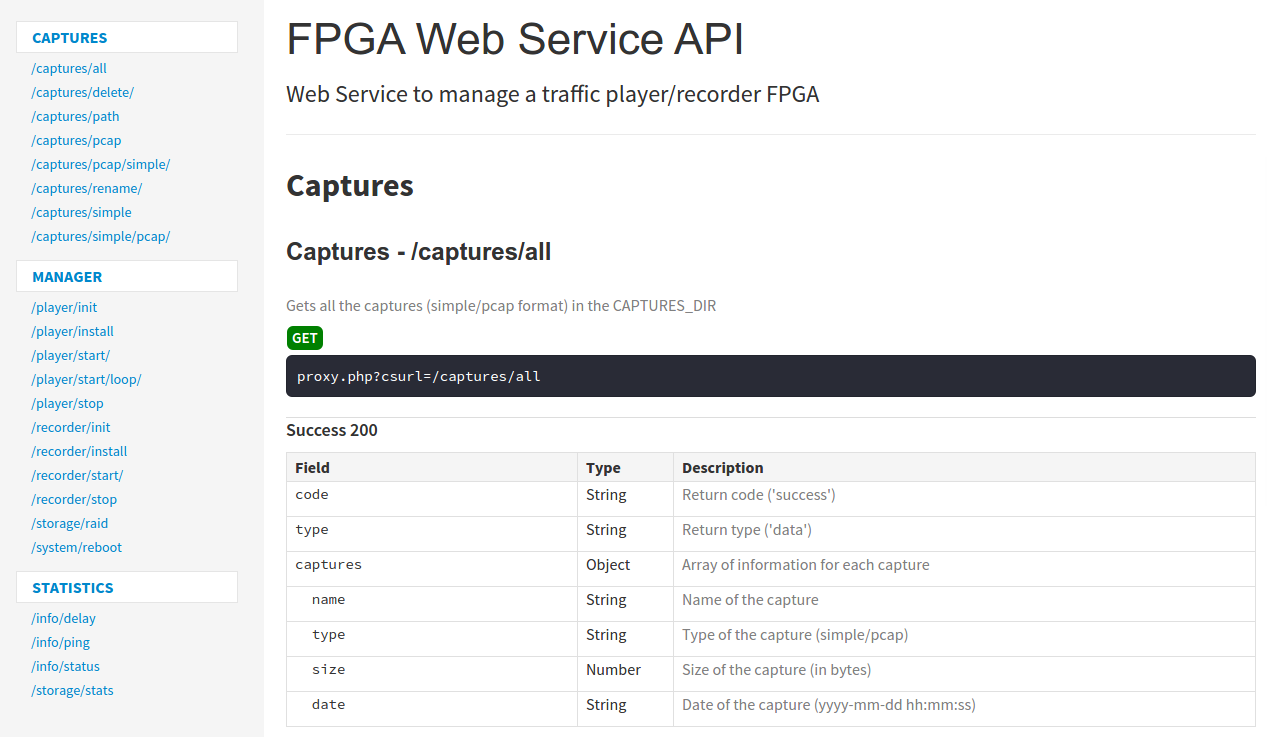
\includegraphics[width=0.95\textwidth,clip=true]{graphics/capturas/docs_backend}
  \caption{Documentación web de la \gls{API} del \gls{servicioweb} \gls{FPGA}.}
  \label{fig:docsbackend}
\end{figure}

\section{Métodos de Gestión \label{extra:api:gestion}}

%
% /system/reboot
%
\subsection{POST /system/reboot}

Reinicia el servidor remoto.
Los parámetros necesarios para la invocación de este método se detallan en la Tabla~\ref{extra:api:reboot:invocacion}.

\begin{table}[H]
\centering
\begin{tabular}{|l|l|l|l|}
\hline
\rowcolor[HTML]{F5F5F5}
\textbf{Parámetro}  & \textbf{Clase} & \textbf{Tipo} & \textbf{Descripción}                  \\ \hline
                    &                &               & Tiempo transcurrido (ms) desde el 1   \\
timestamp           & Cabecera       & Número        & de Enero de 1970 00:00:00 UTC hasta   \\
                    &                &               & ahora (salida de \textit{Date.now()}) \\ \hline
\end{tabular}
\caption{Parámetros de \textit{/system/reboot}}
\label{extra:api:reboot:invocacion}
\end{table}

A continuación se enumeran los distintos códigos de retorno asociados a este método:
\begin{itemize}

\item{\textbf{200 OK:} se ha ordenado con éxito el reinicio del servidor remoto.
Este código de éxito es retornado junto con los parámetros indicados en la Tabla~\ref{extra:api:reboot:ok}.
\begin{table}[H]
\centering
\begin{tabular}{|l|l|l|}
\hline
\rowcolor[HTML]{F5F5F5}
\textbf{Nombre}  & \textbf{Tipo}   & \textbf{Descripción}              \\ \hline
code             & Cadena de texto & Código de retorno ('success')     \\ \hline
type             & Cadena de texto & Código de tipo ('notification')   \\ \hline
description      & Cadena de texto & Descripción del código de retorno \\ \hline
\end{tabular}
\caption{Salida de \textit{/system/reboot} asociada al código 200}
\label{extra:api:reboot:ok}
\end{table}
\begin{minipage}{\textwidth}
Ejemplo de datos asociados al código 200:

\begin{code}[language=json]
{
  "code": "success",
  "type": "notification",
  "description": "The host is rebooting now."
}
\end{code}
\end{minipage}
}

\item{\textbf{412 Error:} el servidor remoto no puede ser reiniciado ya que la \gls{FPGA} está siendo usada.
Este código de error es retornado junto a los parámetros indicados en la Tabla~\ref{extra:api:reboot:error}.
\begin{table}[H]
\centering
\begin{tabular}{|l|l|l|}
\hline
\rowcolor[HTML]{F5F5F5}
\textbf{Nombre}  & \textbf{Tipo}   & \textbf{Descripción}            \\ \hline
code             & Cadena de texto & Código de retorno ('error')     \\ \hline
type             & Cadena de texto & Código de tipo ('notification') \\ \hline
description      & Cadena de texto & Descripción del error           \\ \hline
\end{tabular}
\caption{Salida de \textit{/system/reboot} asociada al código 412}
\label{extra:api:reboot:error}
\end{table}
\begin{minipage}{\textwidth}
Ejemplo de datos asociados al código 412:

\begin{code}[language=json]
{
  "code": "error",
  "type": "notification",
  "description": "The host can not be rebooted. The FPGA is being used."
}
\end{code}
\end{minipage}
}
\end{itemize}

%
% /player/init
%
\subsection{POST /player/init}

Programa la \gls{FPGA} para reproducir \glspl{traza} y reinicia el servidor remoto.
Los parámetros necesarios para la invocación de este método se detallan en la Tabla~\ref{extra:api:playerinit:invocacion}.

\begin{table}[H]
\centering
\begin{tabular}{|l|l|l|l|}
\hline
\rowcolor[HTML]{F5F5F5}
\textbf{Parámetro}  & \textbf{Clase} & \textbf{Tipo} & \textbf{Descripción}                  \\ \hline
                    &                &               & Tiempo transcurrido (ms) desde el 1   \\
timestamp           & Cabecera       & Número        & de Enero de 1970 00:00:00 UTC hasta   \\
                    &                &               & ahora (salida de \textit{Date.now()}) \\ \hline
\end{tabular}
\caption{Parámetros de \textit{/player/init}}
\label{extra:api:playerinit:invocacion}
\end{table}

A continuación se enumeran los distintos códigos de retorno asociados a este método:
\begin{itemize}

\item{\textbf{200 OK:} se ha programado con éxito la \gls{FPGA} para reproducir \glspl{traza} y se va a reiniciar el servidor remoto.
Este código de éxito es retornado junto con los parámetros indicados en la Tabla~\ref{extra:api:playerinit:ok}.
\begin{table}[H]
\centering
\begin{tabular}{|l|l|l|}
\hline
\rowcolor[HTML]{F5F5F5}
\textbf{Nombre}  & \textbf{Tipo}   & \textbf{Descripción}              \\ \hline
code             & Cadena de texto & Código de retorno ('success')     \\ \hline
type             & Cadena de texto & Código de tipo ('notification')   \\ \hline
description      & Cadena de texto & Descripción del código de retorno \\ \hline
\end{tabular}
\caption{Salida de \textit{/player/init} asociada al código 200}
\label{extra:api:playerinit:ok}
\end{table}
\begin{minipage}{\textwidth}
Ejemplo de datos asociados al código 200:

\begin{code}[language=json]
{
  "code": "success",
  "type": "notification",
  "description": "The FPGA has been initialized. The host will reboot now."
}
\end{code}
\end{minipage}
}

\item{\textbf{412 Error:} la \gls{FPGA} no puede ser programada ya que está siendo usada.
Este código de error es retornado junto a los parámetros indicados en la Tabla~\ref{extra:api:playerinit:error}.
\begin{table}[H]
\centering
\begin{tabular}{|l|l|l|}
\hline
\rowcolor[HTML]{F5F5F5}
\textbf{Nombre}  & \textbf{Tipo}   & \textbf{Descripción}                    \\ \hline
code             & Cadena de texto & Código de retorno ('error')             \\ \hline
type             & Cadena de texto & Código de tipo ('fpga\_invalid\_state') \\ \hline
description      & Cadena de texto & Descripción del error                   \\ \hline
\end{tabular}
\caption{Salida de \textit{/player/init} asociada al código 412}
\label{extra:api:playerinit:error}
\end{table}

\begin{minipage}{\textwidth}
Ejemplo de datos asociados al código 412:

\begin{code}[language=json]
{
  "code": "error",
  "type": "fpga_invalid_state",
  "description": "Invalid State. The FPGA is already running, stop it to init the FPGA."
}
\end{code}
\end{minipage}
}

\end{itemize}

%
% /recorder/init
%
\subsection{POST /recorder/init}

Programa la \gls{FPGA} para capturar \glspl{traza} y reinicia el servidor remoto.
Los parámetros necesarios para la invocación de este método se detallan en la Tabla~\ref{extra:api:recorderinit:invocacion}.

\begin{table}[H]
\centering
\begin{tabular}{|l|l|l|l|}
\hline
\rowcolor[HTML]{F5F5F5}
\textbf{Parámetro}  & \textbf{Clase} & \textbf{Tipo} & \textbf{Descripción}                  \\ \hline
                    &                &               & Tiempo transcurrido (ms) desde el 1   \\
timestamp           & Cabecera       & Número        & de Enero de 1970 00:00:00 UTC hasta   \\
                    &                &               & ahora (salida de \textit{Date.now()}) \\ \hline
\end{tabular}
\caption{Parámetros de \textit{/recorder/init}}
\label{extra:api:recorderinit:invocacion}
\end{table}

A continuación se enumeran los distintos códigos de retorno asociados a este método:
\begin{itemize}

\item{\textbf{200 OK:} se ha programado con éxito la \gls{FPGA} para reproducir \glspl{traza} y se va a reiniciar el servidor remoto.
Este código de éxito es retornado junto con los parámetros indicados en la Tabla~\ref{extra:api:recorderinit:ok}.
\begin{table}[H]
\centering
\begin{tabular}{|l|l|l|}
\hline
\rowcolor[HTML]{F5F5F5}
\textbf{Nombre}  & \textbf{Tipo}   & \textbf{Descripción}              \\ \hline
code             & Cadena de texto & Código de retorno ('success')     \\ \hline
type             & Cadena de texto & Código de tipo ('notification')   \\ \hline
description      & Cadena de texto & Descripción del código de retorno \\ \hline
\end{tabular}
\caption{Salida de \textit{/recorder/init} asociada al código 200}
\label{extra:api:recorderinit:ok}
\end{table}
\begin{minipage}{\textwidth}
Ejemplo de datos asociados al código 200:

\begin{code}[language=json]
{
  "code": "success",
  "type": "notification",
  "description": "The FPGA has been initialized. The host will reboot now."
}
\end{code}
\end{minipage}
}

\item{\textbf{412 Error:} la \gls{FPGA} no puede ser programada ya que está siendo usada.
Este código de error es retornado junto a los parámetros indicados en la Tabla~\ref{extra:api:recorderinit:error}.
\begin{table}[H]
\centering
\begin{tabular}{|l|l|l|}
\hline
\rowcolor[HTML]{F5F5F5}
\textbf{Nombre}  & \textbf{Tipo}   & \textbf{Descripción}                    \\ \hline
code             & Cadena de texto & Código de retorno ('error')             \\ \hline
type             & Cadena de texto & Código de tipo ('fpga\_invalid\_state') \\ \hline
description      & Cadena de texto & Descripción del error                   \\ \hline
\end{tabular}
\caption{Salida de \textit{/recorder/init} asociada al código 412}
\label{extra:api:recorderinit:error}
\end{table}

\begin{minipage}{\textwidth}
Ejemplo de datos asociados al código 412:

\begin{code}[language=json]
{
  "code": "error",
  "type": "fpga_invalid_state",
  "description": "Invalid State. The FPGA is already running, stop it to init the FPGA."
}
\end{code}
\end{minipage}
}

\end{itemize}

%
% /player/install
%
\subsection{POST /player/install}
Instala y monta la \gls{FPGA} para reproducir \glspl{traza}.
Los parámetros necesarios para la invocación de este método se detallan en la Tabla~\ref{extra:api:playerinstall:invocacion}.

\begin{table}[H]
\centering
\begin{tabular}{|l|l|l|l|}
\hline
\rowcolor[HTML]{F5F5F5}
\textbf{Parámetro}  & \textbf{Clase} & \textbf{Tipo} & \textbf{Descripción}                  \\ \hline
                    &                &               & Tiempo transcurrido (ms) desde el 1   \\
timestamp           & Cabecera       & Número        & de Enero de 1970 00:00:00 UTC hasta   \\
                    &                &               & ahora (salida de \textit{Date.now()}) \\ \hline
\end{tabular}
\caption{Parámetros de \textit{/player/install}}
\label{extra:api:playerinstall:invocacion}
\end{table}

A continuación se enumeran los distintos códigos de retorno asociados a este método:
\begin{itemize}

\item{\textbf{200 OK:} la \gls{FPGA} se ha instalado y montado con éxito, y está lista para reproducir \glspl{traza}.
Este código de éxito es retornado junto con los parámetros indicados en la Tabla~\ref{extra:api:playerinstall:ok}.
\begin{table}[H]
\centering
\begin{tabular}{|l|l|l|}
\hline
\rowcolor[HTML]{F5F5F5}
\textbf{Nombre}  & \textbf{Tipo}   & \textbf{Descripción}              \\ \hline
code             & Cadena de texto & Código de retorno ('success')     \\ \hline
type             & Cadena de texto & Código de tipo ('notification')   \\ \hline
description      & Cadena de texto & Descripción del código de retorno \\ \hline
\end{tabular}
\caption{Salida de \textit{/player/install} asociada al código 200}
\label{extra:api:playerinstall:ok}
\end{table}
\begin{minipage}{\textwidth}
Ejemplo de datos asociados al código 200:

\begin{code}[language=json]
{
  "code": "success",
  "type": "notification",
  "description": "The FPGA has been mounted and is ready to be used."
}
\end{code}
\end{minipage}
}

\item{\textbf{412 Error:} la \gls{FPGA} no puede ser instalada y montada ya que no ha sido programada.
Este código de error es retornado junto a los parámetros indicados en la Tabla~\ref{extra:api:playerinstall:error}.
\begin{table}[H]
\centering
\begin{tabular}{|l|l|l|}
\hline
\rowcolor[HTML]{F5F5F5}
\textbf{Nombre}  & \textbf{Tipo}   & \textbf{Descripción}                    \\ \hline
code             & Cadena de texto & Código de retorno ('error')             \\ \hline
type             & Cadena de texto & Código de tipo ('fpga\_invalid\_state') \\ \hline
description      & Cadena de texto & Descripción del error                   \\ \hline
\end{tabular}
\caption{Salida de \textit{/player/install} asociada al código 412}
\label{extra:api:playerinstall:error}
\end{table}

\begin{minipage}{\textwidth}
Ejemplo de datos asociados al código 412:

\begin{code}[language=json]
{
  "code": "error",
  "type": "fpga_invalid_state",
  "description": "Invalid State. The FPGA must be programmed before mounted."
}
\end{code}
\end{minipage}
}

\end{itemize}

%
% /recorder/install
%
\subsection{POST /recorder/install}
Instala y monta la \gls{FPGA} para capturar \glspl{traza}.
Los parámetros necesarios para la invocación de este método se detallan en la Tabla~\ref{extra:api:recorderinstall:invocacion}.

\begin{table}[H]
\centering
\begin{tabular}{|l|l|l|l|}
\hline
\rowcolor[HTML]{F5F5F5}
\textbf{Parámetro}  & \textbf{Clase} & \textbf{Tipo} & \textbf{Descripción}                  \\ \hline
                    &                &               & Tiempo transcurrido (ms) desde el 1   \\
timestamp           & Cabecera       & Número        & de Enero de 1970 00:00:00 UTC hasta   \\
                    &                &               & ahora (salida de \textit{Date.now()}) \\ \hline
\end{tabular}
\caption{Parámetros de \textit{/recorder/install}}
\label{extra:api:recorderinstall:invocacion}
\end{table}

A continuación se enumeran los distintos códigos de retorno asociados a este método:
\begin{itemize}

\item{\textbf{200 OK:} la \gls{FPGA} se ha instalado y montado con éxito, y está lista para capturar \glspl{traza}.
Este código de éxito es retornado junto con los parámetros indicados en la Tabla~\ref{extra:api:recorderinstall:ok}.
\begin{table}[H]
\centering
\begin{tabular}{|l|l|l|}
\hline
\rowcolor[HTML]{F5F5F5}
\textbf{Nombre}  & \textbf{Tipo}   & \textbf{Descripción}              \\ \hline
code             & Cadena de texto & Código de retorno ('success')     \\ \hline
type             & Cadena de texto & Código de tipo ('notification')   \\ \hline
description      & Cadena de texto & Descripción del código de retorno \\ \hline
\end{tabular}
\caption{Salida de \textit{/recorder/install} asociada al código 200}
\label{extra:api:recorderinstall:ok}
\end{table}
\begin{minipage}{\textwidth}
Ejemplo de datos asociados al código 200:

\begin{code}[language=json]
{
  "code": "success",
  "type": "notification",
  "description": "The FPGA has been mounted and is ready to be used."
}
\end{code}
\end{minipage}
}

\item{\textbf{412 Error:} la \gls{FPGA} no puede ser instalada y montada ya que no ha sido programada.
Este código de error es retornado junto a los parámetros indicados en la Tabla~\ref{extra:api:recorderinstall:error}.
\begin{table}[H]
\centering
\begin{tabular}{|l|l|l|}
\hline
\rowcolor[HTML]{F5F5F5}
\textbf{Nombre}  & \textbf{Tipo}   & \textbf{Descripción}                    \\ \hline
code             & Cadena de texto & Código de retorno ('error')             \\ \hline
type             & Cadena de texto & Código de tipo ('fpga\_invalid\_state') \\ \hline
description      & Cadena de texto & Descripción del error                   \\ \hline
\end{tabular}
\caption{Salida de \textit{/recorder/install} asociada al código 412}
\label{extra:api:recorderinstall:error}
\end{table}

\begin{minipage}{\textwidth}
Ejemplo de datos asociados al código 412:

\begin{code}[language=json]
{
  "code": "error",
  "type": "fpga_invalid_state",
  "description": "Invalid State. The FPGA must be programmed before mounted."
}
\end{code}
\end{minipage}
}

\end{itemize}

%
% /player/start/:capturename/:mask/:ifg
%
\subsection{POST /player/start/:capturename/:mask/:ifg}
Reproduce una \gls{traza} con los parámetros indicados.
Los parámetros necesarios para la invocación de este método se detallan en la Tabla~\ref{extra:api:playerstart:invocacion}.

\begin{table}[H]
\centering
\begin{tabular}{|l|l|l|l|}
\hline
\rowcolor[HTML]{F5F5F5}
\textbf{Parámetro}  & \textbf{Clase} & \textbf{Tipo}   & \textbf{Descripción}                        \\ \hline
                    &                &                 & Tiempo transcurrido (ms) desde el           \\
timestamp           & Cabecera       & Número          & 1 de Enero de 1970 00:00:00 UTC             \\
                    &                &                 & hasta ahora (salida de \textit{Date.now()}) \\ \hline
capturename         & Parámetro      & Cadena de texto & Nombre de la \gls{traza} a reproducir       \\ \hline
mask                & Parámetro      & Número          & Máscara de reproducción (0-1-2-3)           \\ \hline
ifg                 & Parámetro      & Número          & \gls{IFG} (0 para tasa original)            \\ \hline
\end{tabular}
\caption{Parámetros de \textit{/player/start}}
\label{extra:api:playerstart:invocacion}
\end{table}

A continuación se enumeran los distintos códigos de retorno asociados a este método:
\begin{itemize}

\item{\textbf{200 OK:} la \gls{FPGA} ha empezado a reproducir la \gls{traza} seleccionada con los parámetros indicados.
Este código de éxito es retornado junto con los parámetros indicados en la Tabla~\ref{extra:api:playerstart:ok}.
\begin{table}[H]
\centering
\begin{tabular}{|l|l|l|}
\hline
\rowcolor[HTML]{F5F5F5}
\textbf{Nombre}  & \textbf{Tipo}   & \textbf{Descripción}              \\ \hline
code             & Cadena de texto & Código de retorno ('success')     \\ \hline
type             & Cadena de texto & Código de tipo ('notification')   \\ \hline
description      & Cadena de texto & Descripción del código de retorno \\ \hline
\end{tabular}
\caption{Salida de \textit{/player/start} asociada al código 200}
\label{extra:api:playerstart:ok}
\end{table}
\begin{minipage}{\textwidth}
Ejemplo de datos asociados al código 200:

\begin{code}[language=json]
{
  "code": "success",
  "type": "notification",
  "description": "The FPGA has started playing a capture."
}
\end{code}
\end{minipage}
}

\item{\textbf{400 Error:} la \gls{FPGA} no puede reproducir la \gls{traza} ya que los parámetros pasados son inválidos.
Este código de error es retornado junto a los parámetros indicados en la Tabla~\ref{extra:api:playerstart:error400}.
\begin{table}[H]
\centering
\begin{tabular}{|l|l|l|}
\hline
\rowcolor[HTML]{F5F5F5}
\textbf{Nombre}  & \textbf{Tipo}   & \textbf{Descripción}                    \\ \hline
code             & Cadena de texto & Código de retorno ('error')             \\ \hline
type             & Cadena de texto & Código de tipo ('fpga\_invalid\_state') \\ \hline
description      & Cadena de texto & Descripción del error                   \\ \hline
\end{tabular}
\caption{Salida de \textit{/player/start} asociada al código 400}
\label{extra:api:playerstart:error400}
\end{table}

\begin{minipage}{\textwidth}
Ejemplo de datos asociados al código 400:

\begin{code}[language=json]
{
  "code": "error",
  "type": "notification",
  "description": "Invalid parameters. The FPGA could not start playing a capture."
}
\end{code}
\end{minipage}
}

\item{\textbf{412 Error:} la \gls{FPGA} no puede reproducir la \gls{traza} ya que no ha sido instalada y montada para reproducir \glspl{traza}.
Este código de error es retornado junto a los parámetros indicados en la Tabla~\ref{extra:api:playerstart:error412}.
\begin{table}[H]
\centering
\begin{tabular}{|l|l|l|}
\hline
\rowcolor[HTML]{F5F5F5}
\textbf{Nombre}  & \textbf{Tipo}   & \textbf{Descripción}                    \\ \hline
code             & Cadena de texto & Código de retorno ('error')             \\ \hline
type             & Cadena de texto & Código de tipo ('fpga\_invalid\_state') \\ \hline
description      & Cadena de texto & Descripción del error                   \\ \hline
\end{tabular}
\caption{Salida de \textit{/player/start} asociada al código 412}
\label{extra:api:playerstart:error412}
\end{table}

\begin{minipage}{\textwidth}
Ejemplo de datos asociados al código 412:

\begin{code}[language=json]
{
  "code": "error",
  "type": "fpga_invalid_state",
  "description": "Invalid State. The FPGA is not programmed and mounted as a player."
}
\end{code}
\end{minipage}
}

\end{itemize}

%
% /player/start/loop/:capturename/:mask/:ifg
%
\subsection{POST /player/start/loop/:capturename/:mask/:ifg}
Reproduce en bucle una \gls{traza} con los parámetros indicados.
Los parámetros necesarios para la invocación de este método se detallan en la Tabla~\ref{extra:api:playerstartloop:invocacion}.

\begin{table}[H]
\centering
\begin{tabular}{|l|l|l|l|}
\hline
\rowcolor[HTML]{F5F5F5}
\textbf{Parámetro}  & \textbf{Clase} & \textbf{Tipo}   & \textbf{Descripción}                        \\ \hline
                    &                &                 & Tiempo transcurrido (ms) desde el           \\
timestamp           & Cabecera       & Número          & 1 de Enero de 1970 00:00:00 UTC             \\
                    &                &                 & hasta ahora (salida de \textit{Date.now()}) \\ \hline
capturename         & Parámetro      & Cadena de texto & Nombre de la \gls{traza} a reproducir       \\ \hline
mask                & Parámetro      & Número          & Máscara de reproducción (0-1-2-3)           \\ \hline
ifg                 & Parámetro      & Número          & \gls{IFG} (0 para tasa original)            \\ \hline
\end{tabular}
\caption{Parámetros de \textit{/player/start/loop}}
\label{extra:api:playerstartloop:invocacion}
\end{table}

A continuación se enumeran los distintos códigos de retorno asociados a este método:
\begin{itemize}

\item{\textbf{200 OK:} la \gls{FPGA} ha empezado a reproducir en bucle la \gls{traza} seleccionada con los parámetros indicados.
Este código de éxito es retornado junto con los parámetros indicados en la Tabla~\ref{extra:api:playerstartloop:ok}.
\begin{table}[H]
\centering
\begin{tabular}{|l|l|l|}
\hline
\rowcolor[HTML]{F5F5F5}
\textbf{Nombre}  & \textbf{Tipo}   & \textbf{Descripción}              \\ \hline
code             & Cadena de texto & Código de retorno ('success')     \\ \hline
type             & Cadena de texto & Código de tipo ('notification')   \\ \hline
description      & Cadena de texto & Descripción del código de retorno \\ \hline
\end{tabular}
\caption{Salida de \textit{/player/start/loop} asociada al código 200}
\label{extra:api:playerstartloop:ok}
\end{table}
\begin{minipage}{\textwidth}
Ejemplo de datos asociados al código 200:

\begin{code}[language=json]
{
  "code": "success",
  "type": "notification",
  "description": "The FPGA has started playing a capture."
}
\end{code}
\end{minipage}
}

\item{\textbf{400 Error:} la \gls{FPGA} no puede reproducir la \gls{traza} ya que los parámetros pasados son inválidos.
Este código de error es retornado junto a los parámetros indicados en la Tabla~\ref{extra:api:playerstartloop:error400}.
\begin{table}[H]
\centering
\begin{tabular}{|l|l|l|}
\hline
\rowcolor[HTML]{F5F5F5}
\textbf{Nombre}  & \textbf{Tipo}   & \textbf{Descripción}                    \\ \hline
code             & Cadena de texto & Código de retorno ('error')             \\ \hline
type             & Cadena de texto & Código de tipo ('fpga\_invalid\_state') \\ \hline
description      & Cadena de texto & Descripción del error                   \\ \hline
\end{tabular}
\caption{Salida de \textit{/player/start/loop} asociada al código 400}
\label{extra:api:playerstartloop:error400}
\end{table}

\begin{minipage}{\textwidth}
Ejemplo de datos asociados al código 400:

\begin{code}[language=json]
{
  "code": "error",
  "type": "notification",
  "description": "Invalid parameters. The FPGA could not start playing a capture."
}
\end{code}
\end{minipage}
}

\item{\textbf{412 Error:} la \gls{FPGA} no puede reproducir la \gls{traza} ya que no ha sido instalada y montada para reproducir \glspl{traza}.
Este código de error es retornado junto a los parámetros indicados en la Tabla~\ref{extra:api:playerstartloop:error412}.
\begin{table}[H]
\centering
\begin{tabular}{|l|l|l|}
\hline
\rowcolor[HTML]{F5F5F5}
\textbf{Nombre}  & \textbf{Tipo}   & \textbf{Descripción}                    \\ \hline
code             & Cadena de texto & Código de retorno ('error')             \\ \hline
type             & Cadena de texto & Código de tipo ('fpga\_invalid\_state') \\ \hline
description      & Cadena de texto & Descripción del error                   \\ \hline
\end{tabular}
\caption{Salida de \textit{/player/start/loop} asociada al código 412}
\label{extra:api:playerstartloop:error412}
\end{table}

\begin{minipage}{\textwidth}
Ejemplo de datos asociados al código 412:

\begin{code}[language=json]
{
  "code": "error",
  "type": "fpga_invalid_state",
  "description": "Invalid State. The FPGA is not programmed and mounted as a player."
}
\end{code}
\end{minipage}
}

\end{itemize}

%
% /recorder/start/:capturename/:port/:bytes
%
\subsection{POST /recorder/start/:capturename/:port/:bytes}
Captura una \gls{traza} con los parámetros indicados.
Los parámetros necesarios para la invocación de este método se detallan en la Tabla~\ref{extra:api:recorderstart:invocacion}.

\begin{table}[H]
\centering
\begin{tabular}{|l|l|l|l|}
\hline
\rowcolor[HTML]{F5F5F5}
\textbf{Parámetro}  & \textbf{Clase} & \textbf{Tipo}   & \textbf{Descripción}                         \\ \hline
                    &                &                 & Tiempo transcurrido (ms) desde el            \\
timestamp           & Cabecera       & Número          & 1 de Enero de 1970 00:00:00 UTC              \\
                    &                &                 & hasta ahora (salida de \textit{Date.now()})  \\ \hline
capturename         & Parámetro      & Cadena de texto & Nombre de la \gls{traza} a capturar          \\ \hline
port                & Parámetro      & Número          & Puerto a capturar (0-1-2-3)                  \\ \hline
bytes               & Parámetro      & Número          & Bytes a capturar                             \\ \hline
\end{tabular}
\caption{Parámetros de \textit{/recorder/start}}
\label{extra:api:recorderstart:invocacion}
\end{table}

A continuación se enumeran los distintos códigos de retorno asociados a este método:
\begin{itemize}

\item{\textbf{200 OK:} la \gls{FPGA} ha empezado a capturar una traza con los parámetros indicados.
Este código de éxito es retornado junto con los parámetros indicados en la Tabla~\ref{extra:api:recorderstart:ok}.
\begin{table}[H]
\centering
\begin{tabular}{|l|l|l|}
\hline
\rowcolor[HTML]{F5F5F5}
\textbf{Nombre}  & \textbf{Tipo}   & \textbf{Descripción}              \\ \hline
code             & Cadena de texto & Código de retorno ('success')     \\ \hline
type             & Cadena de texto & Código de tipo ('notification')   \\ \hline
description      & Cadena de texto & Descripción del código de retorno \\ \hline
\end{tabular}
\caption{Salida de \textit{/recorder/start} asociada al código 200}
\label{extra:api:recorderstart:ok}
\end{table}
\begin{minipage}{\textwidth}
Ejemplo de datos asociados al código 200:

\begin{code}[language=json]
{
  "code": "success",
  "type": "notification",
  "description": "The FPGA has started recording data."
}
\end{code}
\end{minipage}
}

\item{\textbf{400 Error:} la \gls{FPGA} no puede empezar a capturar ya que los parámetros pasados son inválidos.
Este código de error es retornado junto a los parámetros indicados en la Tabla~\ref{extra:api:recorderstart:error400}.
\begin{table}[H]
\centering
\begin{tabular}{|l|l|l|}
\hline
\rowcolor[HTML]{F5F5F5}
\textbf{Nombre}  & \textbf{Tipo}   & \textbf{Descripción}                    \\ \hline
code             & Cadena de texto & Código de retorno ('error')             \\ \hline
type             & Cadena de texto & Código de tipo ('fpga\_invalid\_state') \\ \hline
description      & Cadena de texto & Descripción del error                   \\ \hline
\end{tabular}
\caption{Salida de \textit{/recorder/start} asociada al código 400}
\label{extra:api:recorderstart:error400}
\end{table}

\begin{minipage}{\textwidth}
Ejemplo de datos asociados al código 400:

\begin{code}[language=json]
{
  "code": "error",
  "type": "notification",
  "description": "Invalid capture name (must not exist)."
}
\end{code}
\end{minipage}
}

\item{\textbf{412 Error:} la \gls{FPGA} no puede empezar a capturar ya que no ha sido instalada y montada para capturar \glspl{traza}.
Este código de error es retornado junto a los parámetros indicados en la Tabla~\ref{extra:api:recorderstart:error412}.
\begin{table}[H]
\centering
\begin{tabular}{|l|l|l|}
\hline
\rowcolor[HTML]{F5F5F5}
\textbf{Nombre}  & \textbf{Tipo}   & \textbf{Descripción}                    \\ \hline
code             & Cadena de texto & Código de retorno ('error')             \\ \hline
type             & Cadena de texto & Código de tipo ('fpga\_invalid\_state') \\ \hline
description      & Cadena de texto & Descripción del error                   \\ \hline
\end{tabular}
\caption{Salida de \textit{/recorder/start} asociada al código 412}
\label{extra:api:recorderstart:error412}
\end{table}

\begin{minipage}{\textwidth}
Ejemplo de datos asociados al código 412:

\begin{code}[language=json]
{
  "code": "error",
  "type": "fpga_invalid_state",
  "description": "Invalid State. The FPGA is not programmed and mounted as a recorder."
}
\end{code}
\end{minipage}
}

\end{itemize}

%
% /player/stop
%
\subsection{POST /player/stop}
Detiene la reproducción de \gls{traza} en curso.
Los parámetros necesarios para la invocación de este método se detallan en la Tabla~\ref{extra:api:playerstop:invocacion}.

\begin{table}[H]
\centering
\begin{tabular}{|l|l|l|l|}
\hline
\rowcolor[HTML]{F5F5F5}
\textbf{Parámetro}  & \textbf{Clase} & \textbf{Tipo}   & \textbf{Descripción}                         \\ \hline
                    &                &                 & Tiempo transcurrido (ms) desde el            \\
timestamp           & Cabecera       & Número          & 1 de Enero de 1970 00:00:00 UTC              \\
                    &                &                 & hasta ahora (salida de \textit{Date.now()})  \\ \hline
\end{tabular}
\caption{Parámetros de \textit{/player/stop}}
\label{extra:api:playerstop:invocacion}
\end{table}

A continuación se enumeran los distintos códigos de retorno asociados a este método:
\begin{itemize}

\item{\textbf{200 OK:} la \gls{FPGA} ha detenido la reproducción en curso.
Este código de éxito es retornado junto con los parámetros indicados en la Tabla~\ref{extra:api:playerstop:ok}.
\begin{table}[H]
\centering
\begin{tabular}{|l|l|l|}
\hline
\rowcolor[HTML]{F5F5F5}
\textbf{Nombre}  & \textbf{Tipo}   & \textbf{Descripción}              \\ \hline
code             & Cadena de texto & Código de retorno ('success')     \\ \hline
type             & Cadena de texto & Código de tipo ('notification')   \\ \hline
description      & Cadena de texto & Descripción del código de retorno \\ \hline
\end{tabular}
\caption{Salida de \textit{/player/stop} asociada al código 200}
\label{extra:api:playerstop:ok}
\end{table}
\begin{minipage}{\textwidth}
Ejemplo de datos asociados al código 200:

\begin{code}[language=json]
{
  "code": "success",
  "type": "notification",
  "description": "The FPGA has stopped playing a capture."
}
\end{code}
\end{minipage}
}

\item{\textbf{412 Error:} no se ha podido detener la reproducción ya que no existe ninguna en curso.
Este código de error es retornado junto a los parámetros indicados en la Tabla~\ref{extra:api:playerstop:error}.
\begin{table}[H]
\centering
\begin{tabular}{|l|l|l|}
\hline
\rowcolor[HTML]{F5F5F5}
\textbf{Nombre}  & \textbf{Tipo}   & \textbf{Descripción}                    \\ \hline
code             & Cadena de texto & Código de retorno ('error')             \\ \hline
type             & Cadena de texto & Código de tipo ('fpga\_invalid\_state') \\ \hline
description      & Cadena de texto & Descripción del error                   \\ \hline
\end{tabular}
\caption{Salida de \textit{/player/stop} asociada al código 412}
\label{extra:api:playerstop:error}
\end{table}

\begin{minipage}{\textwidth}
Ejemplo de datos asociados al código 412:

\begin{code}[language=json]
{
  "code": "error",
  "type": "fpga_invalid_state",
  "description": "Invalid State. The FPGA is not playing a capture."
}
\end{code}
\end{minipage}
}

\end{itemize}

%
% /recorder/stop
%
\subsection{POST /recorder/stop}
Detiene la captura de \gls{traza} en curso.
Los parámetros necesarios para la invocación de este método se detallan en la Tabla~\ref{extra:api:recorderstop:invocacion}.

\begin{table}[H]
\centering
\begin{tabular}{|l|l|l|l|}
\hline
\rowcolor[HTML]{F5F5F5}
\textbf{Parámetro}  & \textbf{Clase} & \textbf{Tipo}   & \textbf{Descripción}                         \\ \hline
                    &                &                 & Tiempo transcurrido (ms) desde el            \\
timestamp           & Cabecera       & Número          & 1 de Enero de 1970 00:00:00 UTC              \\
                    &                &                 & hasta ahora (salida de \textit{Date.now()})  \\ \hline
\end{tabular}
\caption{Parámetros de \textit{/recorder/stop}}
\label{extra:api:recorderstop:invocacion}
\end{table}

A continuación se enumeran los distintos códigos de retorno asociados a este método:
\begin{itemize}

\item{\textbf{200 OK:} la \gls{FPGA} ha detenido la captura en curso.
Este código de éxito es retornado junto con los parámetros indicados en la Tabla~\ref{extra:api:recorderstop:ok}.
\begin{table}[H]
\centering
\begin{tabular}{|l|l|l|}
\hline
\rowcolor[HTML]{F5F5F5}
\textbf{Nombre}  & \textbf{Tipo}   & \textbf{Descripción}              \\ \hline
code             & Cadena de texto & Código de retorno ('success')     \\ \hline
type             & Cadena de texto & Código de tipo ('notification')   \\ \hline
description      & Cadena de texto & Descripción del código de retorno \\ \hline
\end{tabular}
\caption{Salida de \textit{/recorder/stop} asociada al código 200}
\label{extra:api:recorderstop:ok}
\end{table}
\begin{minipage}{\textwidth}
Ejemplo de datos asociados al código 200:

\begin{code}[language=json]
{
  "code": "success",
  "type": "notification",
  "description": "The FPGA has stopped recording data."
}
\end{code}
\end{minipage}
}

\item{\textbf{412 Error:} no se ha podido detener la captura ya que no existe ninguna en curso.
Este código de error es retornado junto a los parámetros indicados en la Tabla~\ref{extra:api:recorderstop:error}.
\begin{table}[H]
\centering
\begin{tabular}{|l|l|l|}
\hline
\rowcolor[HTML]{F5F5F5}
\textbf{Nombre}  & \textbf{Tipo}   & \textbf{Descripción}                    \\ \hline
code             & Cadena de texto & Código de retorno ('error')             \\ \hline
type             & Cadena de texto & Código de tipo ('fpga\_invalid\_state') \\ \hline
description      & Cadena de texto & Descripción del error                   \\ \hline
\end{tabular}
\caption{Salida de \textit{/recorder/stop} asociada al código 412}
\label{extra:api:recorderstop:error}
\end{table}

\begin{minipage}{\textwidth}
Ejemplo de datos asociados al código 412:

\begin{code}[language=json]
{
  "code": "error",
  "type": "fpga_invalid_state",
  "description": "Invalid State. The FPGA is not recording data."
}
\end{code}
\end{minipage}
}

\end{itemize}

%
% /storage/raid
%
\subsection{DELETE /storage/raid}
Borra (formatea y vuelve a crear) el \gls{RAID} de almacenamiento.
Los parámetros necesarios para la invocación de este método se detallan en la Tabla~\ref{extra:api:storageraid:invocacion}.

\begin{table}[H]
\centering
\begin{tabular}{|l|l|l|l|}
\hline
\rowcolor[HTML]{F5F5F5}
\textbf{Parámetro}  & \textbf{Clase} & \textbf{Tipo}   & \textbf{Descripción}                         \\ \hline
                    &                &                 & Tiempo transcurrido (ms) desde el            \\
timestamp           & Cabecera       & Número          & 1 de Enero de 1970 00:00:00 UTC              \\
                    &                &                 & hasta ahora (salida de \textit{Date.now()})  \\ \hline
\end{tabular}
\caption{Parámetros de \textit{/storage/raid}}
\label{extra:api:storageraid:invocacion}
\end{table}

A continuación se enumeran los distintos códigos de retorno asociados a este método:
\begin{itemize}

\item{\textbf{200 OK:} se ha formateado y vuelto a montar el \gls{RAID} de almacenamiento.
Este código de éxito es retornado junto con los parámetros indicados en la Tabla~\ref{extra:api:storageraid:ok}.
\begin{table}[H]
\centering
\begin{tabular}{|l|l|l|}
\hline
\rowcolor[HTML]{F5F5F5}
\textbf{Nombre}  & \textbf{Tipo}   & \textbf{Descripción}              \\ \hline
code             & Cadena de texto & Código de retorno ('success')     \\ \hline
type             & Cadena de texto & Código de tipo ('notification')   \\ \hline
description      & Cadena de texto & Descripción del código de retorno \\ \hline
\end{tabular}
\caption{Salida de \textit{/storage/raid} asociada al código 200}
\label{extra:api:storageraid:ok}
\end{table}
\begin{minipage}{\textwidth}
Ejemplo de datos asociados al código 200:

\begin{code}[language=json]
{
  "code": "success",
  "type": "notification",
  "description": "The RAID has been formatted and mounted properly."
}
\end{code}
\end{minipage}
}

\item{\textbf{412 Error:} no se ha formateado el \gls{RAID} ya que o está activado o la \gls{FPGA} está en uso.
Este código de error es retornado junto a los parámetros indicados en la Tabla~\ref{extra:api:storageraid:error}.
\begin{table}[H]
\centering
\begin{tabular}{|l|l|l|}
\hline
\rowcolor[HTML]{F5F5F5}
\textbf{Nombre}  & \textbf{Tipo}   & \textbf{Descripción}                    \\ \hline
code             & Cadena de texto & Código de retorno ('error')             \\ \hline
type             & Cadena de texto & Código de tipo ('fpga\_invalid\_state') \\ \hline
description      & Cadena de texto & Descripción del error                   \\ \hline
\end{tabular}
\caption{Salida de \textit{/storage/raid} asociada al código 412}
\label{extra:api:storageraid:error}
\end{table}

\begin{minipage}{\textwidth}
Ejemplo de datos asociados al código 412:

\begin{code}[language=json]
{
  "code": "error",
  "type": "notification",
  "description": "The RAID could not be formatted, RAID configuration option is not set or the FPGA is running."
}
\end{code}
\end{minipage}
}

\end{itemize}



\section{Métodos de Estadísticas \label{extra:api:estadisticas}}

%
% /info/ping
%
\subsection{GET /info/ping}
Método para comprobar si el servidor está operativo.
Este método no requiere parámetros.

A continuación se enumeran los distintos códigos de retorno asociados a este método:
\begin{itemize}

\item{\textbf{200 OK:} servidor operativo.
Este código de éxito es retornado junto con los parámetros indicados en la Tabla~\ref{extra:api:infoping:ok}.
\begin{table}[H]
\centering
\begin{tabular}{|l|l|l|}
\hline
\rowcolor[HTML]{F5F5F5}
\textbf{Nombre}  & \textbf{Tipo}   & \textbf{Descripción}              \\ \hline
code             & Cadena de texto & Código de retorno ('success')     \\ \hline
\end{tabular}
\caption{Salida de \textit{/info/ping} asociada al código 200}
\label{extra:api:infoping:ok}
\end{table}
\begin{minipage}{\textwidth}
Ejemplo de datos asociados al código 200:

\begin{code}[language=json]
{
  "code": "success"
}
\end{code}
\end{minipage}
}

\end{itemize}

%
% /info/delay
%
\subsection{GET /info/delay}
Solicita la diferencia de tiempos existente entre los relojes del cliente y del servidor (en segundos).
Los parámetros necesarios para la invocación de este método se detallan en la Tabla~\ref{extra:api:infodelay:invocacion}.

\begin{table}[H]
\centering
\begin{tabular}{|l|l|l|l|}
\hline
\rowcolor[HTML]{F5F5F5}
\textbf{Parámetro}  & \textbf{Clase} & \textbf{Tipo}   & \textbf{Descripción}                         \\ \hline
                    &                &                 & Tiempo transcurrido (ms) desde el            \\
timestamp           & Cabecera       & Número          & 1 de Enero de 1970 00:00:00 UTC              \\
                    &                &                 & hasta ahora (salida de \textit{Date.now()})  \\ \hline
\end{tabular}
\caption{Parámetros de \textit{/info/delay}}
\label{extra:api:infodelay:invocacion}
\end{table}

A continuación se enumeran los distintos códigos de retorno asociados a este método:
\begin{itemize}

\item{\textbf{200 OK:} solicitud con éxito.
Este código de éxito es retornado junto con los parámetros indicados en la Tabla~\ref{extra:api:infodelay:ok}.
\begin{table}[H]
\centering
\begin{tabular}{|l|l|l|}
\hline
\rowcolor[HTML]{F5F5F5}
\textbf{Nombre}  & \textbf{Tipo}   & \textbf{Descripción}                      \\ \hline
code             & Cadena de texto & Código de retorno ('success')             \\ \hline
type             & Cadena de texto & Código de tipo ('data')                   \\ \hline
delay            & Número          & Diferencia entre relojes (en segundos)    \\ \hline
maxDelay         & Número          & Máxima diferencia permitida (en segundos) \\ \hline
\end{tabular}
\caption{Salida de \textit{/info/delay} asociada al código 200}
\label{extra:api:infodelay:ok}
\end{table}
\begin{minipage}{\textwidth}
Ejemplo de datos asociados al código 200:

\begin{code}[language=json]
 {
   "code": "success",
   "type": "data",
   "delay": 1,
   "maxDelay": 30
 }
\end{code}
\end{minipage}
}

\end{itemize}

%
% /info/status
%
\subsection{GET /info/status}
Solicita el estado actual de la \gls{FPGA}.
Este método no requiere parámetros.

A continuación se enumeran los distintos códigos de retorno asociados a este método:
\begin{itemize}

\item{\textbf{200 OK - hugepages\_off:} opción \textit{HugePages} del sistema operativo no activa.
Este código de éxito es retornado junto con los parámetros indicados en la Tabla~\ref{extra:api:infostatus:hugepagesoff}.
\begin{table}[H]
\centering
\begin{tabular}{|l|l|l|}
\hline
\rowcolor[HTML]{F5F5F5}
\textbf{Nombre}  & \textbf{Tipo}   & \textbf{Descripción}               \\ \hline
code             & Cadena de texto & Código de estado ('hugepages\_off') \\ \hline
description      & Cadena de texto & Descripción del código de estado   \\ \hline
\end{tabular}
\caption{Salida de \textit{/info/status} asociada al código 200 - hugepages\_off}
\label{extra:api:infostatus:hugepagesoff}
\end{table}
\begin{minipage}{\textwidth}
Ejemplo de datos asociados al código 200 - hugepages\_off:

\begin{code}[language=json]
{
  "status": "hugepages_off",
  "description": "HugePages is not enabled. To fix this, the host should be rebooted with this option selected on the GRUB menu."
}
\end{code}
\end{minipage}
}

\item{\textbf{200 OK - init\_off:} la \gls{FPGA} aún no ha sido configurada para captura o reproducción.
Este código de éxito es retornado junto con los parámetros indicados en la Tabla~\ref{extra:api:infostatus:initoff}.
\begin{table}[H]
\centering
\begin{tabular}{|l|l|l|}
\hline
\rowcolor[HTML]{F5F5F5}
\textbf{Nombre}  & \textbf{Tipo}   & \textbf{Descripción}               \\ \hline
code             & Cadena de texto & Código de estado ('init\_off')     \\ \hline
description      & Cadena de texto & Descripción del código de estado   \\ \hline
\end{tabular}
\caption{Salida de \textit{/info/status} asociada al código 200 - init\_off}
\label{extra:api:infostatus:initoff}
\end{table}
\begin{minipage}{\textwidth}
Ejemplo de datos asociados al código 200 - init\_off:

\begin{code}[language=json]
{
  "status": "init_off",
  "description": "The FPGA is not configured either as player or as recorder yet."
}
\end{code}
\end{minipage}
}

\item{\textbf{200 OK - mount\_off:} la \gls{FPGA} está inicializada pero no ha sido montada aún.
Este código de éxito es retornado junto con los parámetros indicados en la Tabla~\ref{extra:api:infostatus:mountoff}.
\begin{table}[H]
\centering
\begin{tabular}{|l|l|l|}
\hline
\rowcolor[HTML]{F5F5F5}
\textbf{Nombre}  & \textbf{Tipo}   & \textbf{Descripción}               \\ \hline
code             & Cadena de texto & Código de estado ('mount\_off')    \\ \hline
description      & Cadena de texto & Descripción del código de estado   \\ \hline
\end{tabular}
\caption{Salida de \textit{/info/status} asociada al código 200 - mount\_off}
\label{extra:api:infostatus:mountoff}
\end{table}
\begin{minipage}{\textwidth}
Ejemplo de datos asociados al código 200 - mount\_off:

\begin{code}[language=json]
{
  "status": "mount_off",
  "description": "The FPGA is initialized but not mounted."
}
\end{code}
\end{minipage}
}

\item{\textbf{200 OK - player\_ready:} la \gls{FPGA} está lista para reproducir una \gls{traza}.
Este código de éxito es retornado junto con los parámetros indicados en la Tabla~\ref{extra:api:infostatus:playerready}.
\begin{table}[H]
\centering
\begin{tabular}{|l|l|l|}
\hline
\rowcolor[HTML]{F5F5F5}
\textbf{Nombre}  & \textbf{Tipo}   & \textbf{Descripción}               \\ \hline
code             & Cadena de texto & Código de estado ('player\_ready') \\ \hline
description      & Cadena de texto & Descripción del código de estado   \\ \hline
\end{tabular}
\caption{Salida de \textit{/info/status} asociada al código 200 - player\_ready}
\label{extra:api:infostatus:playerready}
\end{table}
\begin{minipage}{\textwidth}
Ejemplo de datos asociados al código 200 - player\_ready:

\begin{code}[language=json]
{
  "status": "player_ready",
  "description": "The FPGA is ready to reproduce a capture."
}
\end{code}
\end{minipage}
}

\item{\textbf{200 OK - recorder\_ready:} la \gls{FPGA} está lista para capturar una \gls{traza}.
Este código de éxito es retornado junto con los parámetros indicados en la Tabla~\ref{extra:api:infostatus:recorderready}.
\begin{table}[H]
\centering
\begin{tabular}{|l|l|l|}
\hline
\rowcolor[HTML]{F5F5F5}
\textbf{Nombre}  & \textbf{Tipo}   & \textbf{Descripción}                 \\ \hline
code             & Cadena de texto & Código de estado ('recorder\_ready') \\ \hline
description      & Cadena de texto & Descripción del código de estado     \\ \hline
\end{tabular}
\caption{Salida de \textit{/info/status} asociada al código 200 - recorder\_ready}
\label{extra:api:infostatus:recorderready}
\end{table}
\begin{minipage}{\textwidth}
Ejemplo de datos asociados al código 200 - recorder\_ready:

\begin{code}[language=json]
{
  "status": "player_ready",
  "description": "The FPGA is ready to record a capture."
}
\end{code}
\end{minipage}
}

\item{\textbf{200 OK - playing:} la \gls{FPGA} está reproduciendo una \gls{traza}.
Este código de éxito es retornado junto con los parámetros indicados en la Tabla~\ref{extra:api:infostatus:playing}.
\begin{table}[H]
\centering
\begin{tabular}{|l|l|l|}
\hline
\rowcolor[HTML]{F5F5F5}
\textbf{Nombre}  & \textbf{Tipo}   & \textbf{Descripción}                            \\ \hline
code             & Cadena de texto & Código de estado ('playing')                    \\ \hline
description      & Cadena de texto & Descripción del código de estado                \\ \hline
capture          & Cadena de texto & Nombre de la \gls{traza} en reproducción        \\ \hline
size             & Número          & Tamaño de la \gls{traza} en reproducción        \\ \hline
date             & Cadena de texto & Fecha de la \gls{traza} en reproducción         \\ \hline
elapsed\_time    & Número          & Tiempo transcurrido desde el inicio (segundos)  \\ \hline
packets\_sent    & Número          & Paquetes enviados                               \\ \hline
loop             & Booleano        & \textit{true} si se está reproduciendo en bucle \\ \hline
interframe\_gap  & Número          & \gls{IFG} (0 si es la tasa original)            \\ \hline
mask             & Número          & Máscara de reproducción (0-1-2-3)               \\ \hline
\end{tabular}
\caption{Salida de \textit{/info/status} asociada al código 200 - playing}
\label{extra:api:infostatus:playing}
\end{table}
\begin{minipage}{\textwidth}
Ejemplo de datos asociados al código 200 - playing:

\begin{code}[language=json]
{
  "status": "playing",
  "description": "The FPGA is reproducing a capture.",
  "capture": "my_capture.simple",
  "size": 714131923845,
  "date": "2014-09-29 15:40:34",
  "elapsed_time": 548,
  "packets_sent": 394578123,
  "loop": true,
  "interframe_gap": 0,
  "mask": 3
}
\end{code}
\end{minipage}
}

\item{\textbf{200 OK - recording:} la \gls{FPGA} está capturando una \gls{traza}.
Este código de éxito es retornado junto con los parámetros indicados en la Tabla~\ref{extra:api:infostatus:recording}.
\begin{table}[H]
\centering
\begin{tabular}{|l|l|l|}
\hline
\rowcolor[HTML]{F5F5F5}
\textbf{Nombre}  & \textbf{Tipo}   & \textbf{Descripción}                            \\ \hline
code             & Cadena de texto & Código de estado ('recording')                  \\ \hline
description      & Cadena de texto & Descripción del código de estado                \\ \hline
capture          & Cadena de texto & Nombre de la \gls{traza} a capturar             \\ \hline
elapsed\_time    & Número          & Tiempo transcurrido desde el inicio (segundos)  \\ \hline
bytes\_captured  & Número          & Bytes capturados                                \\ \hline
bytes\_total     & Número          & Total de bytes a capturar                       \\ \hline
port             & Número          & Puerto que está siendo capturado (0-1-2-3)      \\ \hline
\end{tabular}
\caption{Salida de \textit{/info/status} asociada al código 200 - recording}
\label{extra:api:infostatus:recording}
\end{table}
\begin{minipage}{\textwidth}
Ejemplo de datos asociados al código 200 - recording:

\begin{code}[language=json]
{
  "status": "recording",
  "description": "The FPGA is recording a capture.",
  "capture": "flows_test",
  "elapsed_time": 447,
  "bytes_captured": 5984234711238,
  "bytes_total": 234856352341724128,
  "port": 2
}
\end{code}
\end{minipage}
}

\end{itemize}

%
% /storage/stats
%
\subsection{GET /storage/stats}
Solicita estadísticas del almacenamiento.
Este método no requiere parámetros.

A continuación se enumeran los distintos códigos de retorno asociados a este método:
\begin{itemize}

\item{\textbf{200 OK:} estadísticas obtenidas.
Este código de éxito es retornado junto con los parámetros indicados en la Tabla~\ref{extra:api:storagestats:ok}.
\begin{table}[H]
\centering
\begin{tabular}{|l|l|l|}
\hline
\rowcolor[HTML]{F5F5F5}
\textbf{Nombre}                & \textbf{Tipo}   & \textbf{Descripción}                        \\ \hline
code                           & Cadena de texto & Código de retorno ('success')               \\ \hline
type                           & Cadena de texto & Código de tipo ('data')                     \\ \hline
total\_space                   & Número          & Espacio total (en bytes)                    \\ \hline
used\_space                    & Número          & Espacio utilizado (en bytes)                \\ \hline
raid\_stats                    & Objeto          & Estadísticas del \gls{RAID}                 \\ \hline
raid\_stats.raid\_active       & Booleano        & \textit{true} si el \gls{RAID} está activo  \\ \hline
raid\_stats.write\_speed       & Número          & Velocidad de escritura del \gls{RAID} (B/s) \\ \hline
raid\_stats.disks              & Vector          & Vector con estadísticas de cada disco       \\ \hline
raid\_stats.disks.name         & Cadena de texto & Nombre del disco                            \\ \hline
raid\_stats.disks.write\_speed & Número          & Velocidad de escritura del disco (B/s)      \\ \hline
\end{tabular}
\caption{Salida de \textit{/storage/stats} asociada al código 200}
\label{extra:api:storagestats:ok}
\end{table}
\begin{minipage}{\textwidth}
Ejemplo de datos asociados al código 200:

\begin{code}[language=json]
{
  "code": "success",
  "type": "data",
  "total_space": 240972104,
  "used_space": 70828412,
  "raid_stats": {
    "raid_active": true,
    "raid_name": "/dev/md0",
    "write_speed": 4051114978890,
    "disks": [
      {
        "name": "/dev/sdc",
        "write_speed": 15435231341
      },
      {
        "name": "/dev/sdd",
        "write_speed": 32112351239
      },
      {
        "name": "/dev/sde",
        "write_speed": 19123843109
      }
    ]
  }
}
\end{code}
\end{minipage}
}

\end{itemize}

\section{Métodos de Trazas \label{extra:api:trazas}}

%
% /captures/all
%
\subsection{GET /captures/all}
Solicita información sobre todas las \glspl{traza} disponibles.
Este método no requiere parámetros.

A continuación se enumeran los distintos códigos de retorno asociados a este método:
\begin{itemize}

\item{\textbf{200 OK:} información de las \glspl{traza} obtenida.
Este código de éxito es retornado junto con los parámetros indicados en la Tabla~\ref{extra:api:capturesall:ok}.
\begin{table}[H]
\centering
\begin{tabular}{|l|l|l|}
\hline
\rowcolor[HTML]{F5F5F5}
\textbf{Nombre}                & \textbf{Tipo}   & \textbf{Descripción}                            \\ \hline
code                           & Cadena de texto & Código de retorno ('success')                   \\ \hline
type                           & Cadena de texto & Código de tipo ('data')                         \\ \hline
captures                       & Vector          & Vector con información de las \glspl{traza}     \\ \hline
captures.name                  & Cadena de texto & Nombre de la \gls{traza}                        \\ \hline
captures.type                  & Cadena de texto & Tipo de \gls{traza} (\gls{simple} o \gls{pcap}) \\ \hline
captures.size                  & Número          & Tamaño de la \gls{traza} (en bytes)             \\ \hline
captures.date                  & Cadena de texto & Fecha de la \gls{traza}                         \\ \hline
\end{tabular}
\caption{Salida de \textit{/captures/all} asociada al código 200}
\label{extra:api:capturesall:ok}
\end{table}
\begin{minipage}{\textwidth}
Ejemplo de datos asociados al código 200:

\begin{code}[language=json]
{
  "code": "success",
  "type": "data",
  "captures": [
    {
      "name": "flows_crc",
      "type": "simple",
      "size": 956092345897,
      "date": "2015-03-05 13:42:15"
    },
    {
      "name": "my_capture.simple",
      "type": "pcap",
      "size": 4981234712,
      "date": "2015-02-16 11:08:18"
    },
    {
      "name": "capture_labs.pcap",
      "type": "pcap",
      "size": 30563653141,
      "date": "2015-01-11 17:32:19"
    }
  ]
}
\end{code}
\end{minipage}
}

\end{itemize}

%
% /captures/simple
%
\subsection{GET /captures/simple}
Solicita información sobre todas las \glspl{traza} en formato \gls{simple} disponibles.
Este método no requiere parámetros.

A continuación se enumeran los distintos códigos de retorno asociados a este método:
\begin{itemize}

\item{\textbf{200 OK:} información de las \glspl{traza} en formato \gls{simple} obtenida.
Este código de éxito es retornado junto con los parámetros indicados en la Tabla~\ref{extra:api:capturessimple:ok}.
\begin{table}[H]
\centering
\begin{tabular}{|l|l|l|}
\hline
\rowcolor[HTML]{F5F5F5}
\textbf{Nombre}                & \textbf{Tipo}   & \textbf{Descripción}                            \\ \hline
code                           & Cadena de texto & Código de retorno ('success')                   \\ \hline
type                           & Cadena de texto & Código de tipo ('data')                         \\ \hline
captures                       & Vector          & Vector con información de las \glspl{traza}     \\ \hline
captures.name                  & Cadena de texto & Nombre de la \gls{traza}                        \\ \hline
captures.type                  & Cadena de texto & Tipo de \gls{traza} (\gls{simple})              \\ \hline
captures.size                  & Número          & Tamaño de la \gls{traza} (en bytes)             \\ \hline
captures.date                  & Cadena de texto & Fecha de la \gls{traza}                         \\ \hline
\end{tabular}
\caption{Salida de \textit{/captures/simple} asociada al código 200}
\label{extra:api:capturessimple:ok}
\end{table}
\begin{minipage}{\textwidth}
Ejemplo de datos asociados al código 200:

\begin{code}[language=json]
{
  "code": "success",
  "type": "data",
  "captures": [
    {
      "name": "flows_crc",
      "type": "simple",
      "size": 956092345897,
      "date": "2015-03-05 13:42:15"
    }
  ]
}
\end{code}
\end{minipage}
}

\end{itemize}

%
% /captures/pcap
%
\subsection{GET /captures/pcap}
Solicita información sobre todas las \glspl{traza} en formato \gls{pcap} disponibles.
Este método no requiere parámetros.

A continuación se enumeran los distintos códigos de retorno asociados a este método:
\begin{itemize}

\item{\textbf{200 OK:} información de las \glspl{traza} en formato \gls{pcap} obtenida.
Este código de éxito es retornado junto con los parámetros indicados en la Tabla~\ref{extra:api:capturespcap:ok}.
\begin{table}[H]
\centering
\begin{tabular}{|l|l|l|}
\hline
\rowcolor[HTML]{F5F5F5}
\textbf{Nombre}                & \textbf{Tipo}   & \textbf{Descripción}                            \\ \hline
code                           & Cadena de texto & Código de retorno ('success')                   \\ \hline
type                           & Cadena de texto & Código de tipo ('data')                         \\ \hline
captures                       & Vector          & Vector con información de las \glspl{traza}     \\ \hline
captures.name                  & Cadena de texto & Nombre de la \gls{traza}                        \\ \hline
captures.type                  & Cadena de texto & Tipo de \gls{traza} (\gls{pcap})                \\ \hline
captures.size                  & Número          & Tamaño de la \gls{traza} (en bytes)             \\ \hline
captures.date                  & Cadena de texto & Fecha de la \gls{traza}                         \\ \hline
\end{tabular}
\caption{Salida de \textit{/captures/pcap} asociada al código 200}
\label{extra:api:capturespcap:ok}
\end{table}
\begin{minipage}{\textwidth}
Ejemplo de datos asociados al código 200:

\begin{code}[language=json]
{
  "code": "success",
  "type": "data",
  "captures": [
    {
      "name": "my_capture.simple",
      "type": "pcap",
      "size": 4981234712,
      "date": "2015-02-16 11:08:18"
    },
    {
      "name": "capture_labs.pcap",
      "type": "pcap",
      "size": 30563653141,
      "date": "2015-01-11 17:32:19"
    }
  ]
}
\end{code}
\end{minipage}
}

\end{itemize}

%
% /captures/path
%
\subsection{GET /captures/path}
Solicita información sobre dónde se almacenan las \glspl{traza}.
Este método no requiere parámetros.

A continuación se enumeran los distintos códigos de retorno asociados a este método:
\begin{itemize}

\item{\textbf{200 OK:} información de las \glspl{traza} en formato \gls{pcap} obtenida.
Este código de éxito es retornado junto con los parámetros indicados en la Tabla~\ref{extra:api:capturespath:ok}.
\begin{table}[H]
\centering
\begin{tabular}{|l|l|l|}
\hline
\rowcolor[HTML]{F5F5F5}
\textbf{Nombre}                & \textbf{Tipo}   & \textbf{Descripción}                            \\ \hline
code                           & Cadena de texto & Código de retorno ('success')                   \\ \hline
type                           & Cadena de texto & Código de tipo ('data')                         \\ \hline
path                           & Cadena de texto & Carpeta donde se almacenan las \glspl{traza}    \\ \hline
\end{tabular}
\caption{Salida de \textit{/captures/path} asociada al código 200}
\label{extra:api:capturespath:ok}
\end{table}
\begin{minipage}{\textwidth}
Ejemplo de datos asociados al código 200:

\begin{code}[language=json]
{
  "code": "success",
  "type": "data",
  "path": "/dev/raid/captures/"
}
\end{code}
\end{minipage}
}

\end{itemize}

%
% /captures/rename/:oldname/:newname
%
\subsection{PUT /captures/rename/:oldname/:newname}
Renombra una \gls{traza}.
Los parámetros necesarios para la invocación de este método se detallan en la Tabla~\ref{extra:api:capturesrename:invocacion}.

\begin{table}[H]
\centering
\begin{tabular}{|l|l|l|l|}
\hline
\rowcolor[HTML]{F5F5F5}
\textbf{Parámetro}  & \textbf{Clase} & \textbf{Tipo}   & \textbf{Descripción}                        \\ \hline
                    &                &                 & Tiempo transcurrido (ms) desde el           \\
timestamp           & Cabecera       & Número          & 1 de Enero de 1970 00:00:00 UTC             \\
                    &                &                 & hasta ahora (salida de \textit{Date.now()}) \\ \hline
oldname             & Parámetro      & Cadena de texto & Nombre de la \gls{traza} a renombrar        \\ \hline
newname             & Parámetro      & Cadena de texto & Nuevo nombre de la \gls{traza}              \\ \hline
\end{tabular}
\caption{Parámetros de \textit{/captures/rename}}
\label{extra:api:capturesrename:invocacion}
\end{table}

A continuación se enumeran los distintos códigos de retorno asociados a este método:
\begin{itemize}

\item{\textbf{200 OK:} la \gls{traza} se ha renombrado con éxito.
Este código de éxito es retornado junto con los parámetros indicados en la Tabla~\ref{extra:api:capturesrename:ok}.
\begin{table}[H]
\centering
\begin{tabular}{|l|l|l|}
\hline
\rowcolor[HTML]{F5F5F5}
\textbf{Nombre}  & \textbf{Tipo}   & \textbf{Descripción}              \\ \hline
code             & Cadena de texto & Código de retorno ('success')     \\ \hline
type             & Cadena de texto & Código de tipo ('notification')   \\ \hline
description      & Cadena de texto & Descripción del código de retorno \\ \hline
\end{tabular}
\caption{Salida de \textit{/captures/rename} asociada al código 200}
\label{extra:api:capturesrename:ok}
\end{table}
\begin{minipage}{\textwidth}
Ejemplo de datos asociados al código 200:

\begin{code}[language=json]
{
  "code": "success",
  "type": "notification",
  "description": "The capture has been successfully renamed."
}
\end{code}
\end{minipage}
}

\item{\textbf{400 Error:} no se ha podido renombrar la \gls{traza} (está en uso o el nuevo nombre no es válido).
Este código de error es retornado junto a los parámetros indicados en la Tabla~\ref{extra:api:capturesrename:error}.
\begin{table}[H]
\centering
\begin{tabular}{|l|l|l|}
\hline
\rowcolor[HTML]{F5F5F5}
\textbf{Nombre}  & \textbf{Tipo}   & \textbf{Descripción}            \\ \hline
code             & Cadena de texto & Código de retorno ('error')     \\ \hline
type             & Cadena de texto & Código de tipo ('notification') \\ \hline
description      & Cadena de texto & Descripción del error           \\ \hline
\end{tabular}
\caption{Salida de \textit{/captures/rename} asociada al código 400}
\label{extra:api:capturesrename:error}
\end{table}
\begin{minipage}{\textwidth}
Ejemplo de datos asociados al código 400:

\begin{code}[language=json]
{
  "code": "error",
  "type": "notification",
  "description": "The capture could not be renamed. The new name is already in use or the capture is being used."
}
\end{code}
\end{minipage}
}
\end{itemize}

%
% /captures/simple/pcap/:name/:convertedname
%
\subsection{PUT /captures/simple/pcap/:name/:convertedname}
Convierte una \gls{traza} de formato \gls{simple} a formato \gls{pcap}.
Los parámetros necesarios para la invocación de este método se detallan en la Tabla~\ref{extra:api:capturessimplepcap:invocacion}.

\begin{table}[H]
\centering
\begin{tabular}{|l|l|l|l|}
\hline
\rowcolor[HTML]{F5F5F5}
\textbf{Parámetro}  & \textbf{Clase} & \textbf{Tipo}   & \textbf{Descripción}                        \\ \hline
                    &                &                 & Tiempo transcurrido (ms) desde el           \\
timestamp           & Cabecera       & Número          & 1 de Enero de 1970 00:00:00 UTC             \\
                    &                &                 & hasta ahora (salida de \textit{Date.now()}) \\ \hline
name                & Parámetro      & Cadena de texto & Nombre de la \gls{traza} a convertir        \\ \hline
convertedname       & Parámetro      & Cadena de texto & Nombre de la \gls{traza} convertida         \\ \hline
\end{tabular}
\caption{Parámetros de \textit{/captures/simple/pcap}}
\label{extra:api:capturessimplepcap:invocacion}
\end{table}

A continuación se enumeran los distintos códigos de retorno asociados a este método:
\begin{itemize}

\item{\textbf{200 OK:} la \gls{traza} se ha convertido con éxito.
Este código de éxito es retornado junto con los parámetros indicados en la Tabla~\ref{extra:api:capturessimplepcap:ok}.
\begin{table}[H]
\centering
\begin{tabular}{|l|l|l|}
\hline
\rowcolor[HTML]{F5F5F5}
\textbf{Nombre}  & \textbf{Tipo}   & \textbf{Descripción}              \\ \hline
code             & Cadena de texto & Código de retorno ('success')     \\ \hline
type             & Cadena de texto & Código de tipo ('notification')   \\ \hline
description      & Cadena de texto & Descripción del código de retorno \\ \hline
\end{tabular}
\caption{Salida de \textit{/captures/simple/pcap} asociada al código 200}
\label{extra:api:capturessimplepcap:ok}
\end{table}
\begin{minipage}{\textwidth}
Ejemplo de datos asociados al código 200:

\begin{code}[language=json]
{
  "code": "success",
  "type": "notification",
  "description": "The capture has been successfully converted."
}
\end{code}
\end{minipage}
}

\item{\textbf{400 Error:} no se ha podido convertir la \gls{traza} (el nuevo nombre no es válido o la \gls{traza} original no está en formato \gls{simple}).
Este código de error es retornado junto a los parámetros indicados en la Tabla~\ref{extra:api:capturessimplepcap:error}.
\begin{table}[H]
\centering
\begin{tabular}{|l|l|l|}
\hline
\rowcolor[HTML]{F5F5F5}
\textbf{Nombre}  & \textbf{Tipo}   & \textbf{Descripción}            \\ \hline
code             & Cadena de texto & Código de retorno ('error')     \\ \hline
type             & Cadena de texto & Código de tipo ('notification') \\ \hline
description      & Cadena de texto & Descripción del error           \\ \hline
\end{tabular}
\caption{Salida de \textit{/captures/simple/pcap} asociada al código 400}
\label{extra:api:capturessimplepcap:error}
\end{table}
\begin{minipage}{\textwidth}
Ejemplo de datos asociados al código 400:

\begin{code}[language=json]
{
  "code": "error",
  "type": "notification",
  "description": "The capture could not be converted. The capture has not a valid format or name, or the new name is already in use."
}
\end{code}
\end{minipage}
}
\end{itemize}

%
% /captures/pcap/simple/:name/:convertedname
%
\subsection{PUT /captures/pcap/simple/:name/:convertedname}
Convierte una \gls{traza} de formato \gls{pcap} a formato \gls{simple}.
Los parámetros necesarios para la invocación de este método se detallan en la Tabla~\ref{extra:api:capturespcapsimple:invocacion}.

\begin{table}[H]
\centering
\begin{tabular}{|l|l|l|l|}
\hline
\rowcolor[HTML]{F5F5F5}
\textbf{Parámetro}  & \textbf{Clase} & \textbf{Tipo}   & \textbf{Descripción}                        \\ \hline
                    &                &                 & Tiempo transcurrido (ms) desde el           \\
timestamp           & Cabecera       & Número          & 1 de Enero de 1970 00:00:00 UTC             \\
                    &                &                 & hasta ahora (salida de \textit{Date.now()}) \\ \hline
name                & Parámetro      & Cadena de texto & Nombre de la \gls{traza} a convertir        \\ \hline
convertedname       & Parámetro      & Cadena de texto & Nombre de la \gls{traza} convertida         \\ \hline
\end{tabular}
\caption{Parámetros de \textit{/captures/pcap/simple}}
\label{extra:api:capturespcapsimple:invocacion}
\end{table}

A continuación se enumeran los distintos códigos de retorno asociados a este método:
\begin{itemize}

\item{\textbf{200 OK:} la \gls{traza} se ha convertido con éxito.
Este código de éxito es retornado junto con los parámetros indicados en la Tabla~\ref{extra:api:capturespcapsimple:ok}.
\begin{table}[H]
\centering
\begin{tabular}{|l|l|l|}
\hline
\rowcolor[HTML]{F5F5F5}
\textbf{Nombre}  & \textbf{Tipo}   & \textbf{Descripción}              \\ \hline
code             & Cadena de texto & Código de retorno ('success')     \\ \hline
type             & Cadena de texto & Código de tipo ('notification')   \\ \hline
description      & Cadena de texto & Descripción del código de retorno \\ \hline
\end{tabular}
\caption{Salida de \textit{/captures/pcap/simple} asociada al código 200}
\label{extra:api:capturespcapsimple:ok}
\end{table}
\begin{minipage}{\textwidth}
Ejemplo de datos asociados al código 200:

\begin{code}[language=json]
{
  "code": "success",
  "type": "notification",
  "description": "The capture has been successfully converted."
}
\end{code}
\end{minipage}
}

\item{\textbf{400 Error:} no se ha podido convertir la \gls{traza} (el nuevo nombre no es válido o la \gls{traza} original no está en formato \gls{pcap}).
Este código de error es retornado junto a los parámetros indicados en la Tabla~\ref{extra:api:capturespcapsimple:error}.
\begin{table}[H]
\centering
\begin{tabular}{|l|l|l|}
\hline
\rowcolor[HTML]{F5F5F5}
\textbf{Nombre}  & \textbf{Tipo}   & \textbf{Descripción}            \\ \hline
code             & Cadena de texto & Código de retorno ('error')     \\ \hline
type             & Cadena de texto & Código de tipo ('notification') \\ \hline
description      & Cadena de texto & Descripción del error           \\ \hline
\end{tabular}
\caption{Salida de \textit{/captures/pcap/simple} asociada al código 400}
\label{extra:api:capturespcapsimple:error}
\end{table}
\begin{minipage}{\textwidth}
Ejemplo de datos asociados al código 400:

\begin{code}[language=json]
{
  "code": "error",
  "type": "notification",
  "description": "The capture could not be converted. The capture has not a valid format or name, or the new name is already in use."
}
\end{code}
\end{minipage}
}
\end{itemize}

%
% /captures/delete/:name
%
\subsection{DELETE /captures/delete/:name}
Borra una \gls{traza}.
Los parámetros necesarios para la invocación de este método se detallan en la Tabla~\ref{extra:api:capturesdelete:invocacion}.

\begin{table}[H]
\centering
\begin{tabular}{|l|l|l|l|}
\hline
\rowcolor[HTML]{F5F5F5}
\textbf{Parámetro}  & \textbf{Clase} & \textbf{Tipo}   & \textbf{Descripción}                        \\ \hline
                    &                &                 & Tiempo transcurrido (ms) desde el           \\
timestamp           & Cabecera       & Número          & 1 de Enero de 1970 00:00:00 UTC             \\
                    &                &                 & hasta ahora (salida de \textit{Date.now()}) \\ \hline
name                & Parámetro      & Cadena de texto & Nombre de la \gls{traza} a borrar           \\ \hline
\end{tabular}
\caption{Parámetros de \textit{/captures/delete}}
\label{extra:api:capturesdelete:invocacion}
\end{table}

A continuación se enumeran los distintos códigos de retorno asociados a este método:
\begin{itemize}

\item{\textbf{200 OK:} la \gls{traza} se ha borrado con éxito.
Este código de éxito es retornado junto con los parámetros indicados en la Tabla~\ref{extra:api:capturesdelete:ok}.
\begin{table}[H]
\centering
\begin{tabular}{|l|l|l|}
\hline
\rowcolor[HTML]{F5F5F5}
\textbf{Nombre}  & \textbf{Tipo}   & \textbf{Descripción}              \\ \hline
code             & Cadena de texto & Código de retorno ('success')     \\ \hline
type             & Cadena de texto & Código de tipo ('notification')   \\ \hline
description      & Cadena de texto & Descripción del código de retorno \\ \hline
\end{tabular}
\caption{Salida de \textit{/captures/delete} asociada al código 200}
\label{extra:api:capturesdelete:ok}
\end{table}
\begin{minipage}{\textwidth}
Ejemplo de datos asociados al código 200:

\begin{code}[language=json]
{
  "code": "success",
  "type": "notification",
  "description": "The capture has been successfully deleted."
}
\end{code}
\end{minipage}
}

\item{\textbf{400 Error:} no se ha podido borrar la \gls{traza} (está en uso o no existe).
Este código de error es retornado junto a los parámetros indicados en la Tabla~\ref{extra:api:capturesdelete:error}.
\begin{table}[H]
\centering
\begin{tabular}{|l|l|l|}
\hline
\rowcolor[HTML]{F5F5F5}
\textbf{Nombre}  & \textbf{Tipo}   & \textbf{Descripción}            \\ \hline
code             & Cadena de texto & Código de retorno ('error')     \\ \hline
type             & Cadena de texto & Código de tipo ('notification') \\ \hline
description      & Cadena de texto & Descripción del error           \\ \hline
\end{tabular}
\caption{Salida de \textit{/captures/delete} asociada al código 400}
\label{extra:api:capturesdelete:error}
\end{table}
\begin{minipage}{\textwidth}
Ejemplo de datos asociados al código 400:

\begin{code}[language=json]
{
  "code": "error",
  "type": "notification",
  "description": "The capture could not be deleted (it is in use or it does not exist)."
}
\end{code}
\end{minipage}
}
\end{itemize}


% Fin del documento
\end{document}
